\documentclass[aspectratio=169,11pt,usenames,dvipsnames]{beamer}

% \usepackage[colorlinks=true,linkcolor=customblue, citecolor=hpred,urlcolor=customlightblue]{hyperref}

\usetheme{simple}

% packages
\usepackage{mathrsfs}  
\usepackage{cancel}
\usepackage{smartdiagram}
\usesmartdiagramlibrary{additions}

\tikzset{bubble node/.append style={
        draw=none, 
    }
}
\tikzset{bubble center node/.append style={
        draw=none, 
    }
}

% \tikzset{myarrow/.style={-{Stealth[length=2.5mm,width=2.5mm]}, line width=1.5pt}}
\tikzset{myarrow/.style={-Stealth}, line width=2.0pt}
\tikzset{
    myleftrightarrow/.style={Stealth-Stealth, line width=2.0pt}
}

% \usepackage{caption}
% \usepackage{tikz}

\makeatother
\renewcommand{\thefootnote}{\color{customblue}\faPaperPlaneO}
\makeatletter

\newcommand{\symfootnote}[1]{%
\let\oldthefootnote=\thefootnote%
\stepcounter{mpfootnote}%
\addtocounter{footnote}{-1}%
\renewcommand{\thefootnote}{$\dagger$}%
\footnote{#1}%
\let\thefootnote=\oldthefootnote%
}

\newcommand\blfootnote[1]{%
  \begingroup
  \renewcommand\thefootnote{}\footnote{#1}%
  \addtocounter{footnote}{-1}%
  \endgroup
}

\usepackage{xcolor}
\usepackage{graphicx}
\usepackage{empheq}
\usepackage{physics}
\usepackage{svg}
\usepackage{bm}
\usepackage{amsmath}
\usepackage{amssymb}
\usepackage{annotate-equations}

\usepackage{appendixnumberbeamer}

\usepackage{relsize}

\usepackage{fontawesome}


\usetikzlibrary{decorations.pathreplacing, decorations.pathmorphing,calc,arrows,positioning}

% Custom colors

\definecolor{isred}{HTML}{81182d}
\definecolor{hpred}{HTML}{712A27}
\definecolor{hpblue}{HTML}{44545c}

\definecolor{indicoplen}{HTML}{f8f2e8}
\definecolor{indicopar}{HTML}{dfebff}

\definecolor{darkqhat}{HTML}{aa3d3e}
\definecolor{lightqhat}{HTML}{fabfc6}

\definecolor{customblue}{HTML}{3c9bb3}
\definecolor{customgreen}{HTML}{117877}
\definecolor{custompink}{HTML}{c35861}
\definecolor{customred}{HTML}{9d1700}
\definecolor{customyellow}{HTML}{e0ad04}
\definecolor{lightgray}{HTML}{a6a4a4}

\definecolor{lightcustomblue}{HTML}{aad1e6}
\definecolor{lightpink}{HTML}{ba8489}

\definecolor{starrymain}{HTML}{3B5B65}
\definecolor{starrysecond}{HTML}{719593}

\definecolor{ektgreen}{HTML}{047c73}
\definecolor{ektblue}{HTML}{065680}

\definecolor{angcorr}{HTML}{502d7e}

\definecolor{pinky}{HTML}{c35861}
\definecolor{ming}{HTML}{117877}

\definecolor{jyublue}{HTML}{002145}
\definecolor{jyured}{HTML}{e13126}
\definecolor{jyulightblue}{HTML}{909eae}

\definecolor{paldarkblue}{HTML}{0d1f2d}
\definecolor{pallightblue}{HTML}{2f586e}
\definecolor{paldarkgold}{HTML}{d2973b}
\definecolor{pallightgold}{HTML}{e8ca84}
\definecolor{palred}{HTML}{8c0e0f}

\definecolor{palblue}{HTML}{0d3672}
\definecolor{palteal}{HTML}{406f6b}
\definecolor{palgold}{HTML}{b99146}
\definecolor{palviolet}{HTML}{9F87AF}

\definecolor{raapink}{HTML}{ce93b5}
\definecolor{raablue}{HTML}{5c93b8}

\definecolor{bayesian}{HTML}{B2B6FF}

\definecolor{isback}{HTML}{192128}
\definecolor{isgold}{HTML}{c59a7a}

\usepackage{etoolbox}
\setbeamertemplate{blocks}[rounded][shadow=false]
\setbeamercolor{block title}{use=structure,fg=palteal,bg=palteal!10}
\setbeamercolor{block body}{parent=normal text,use=block title,bg=palteal!10}

\usepackage[most]{tcolorbox}
\newtcolorbox{mybox}[2][]{tcbox width=auto limited,capture=hbox,colbacktitle=red!10!white, colback=blue!10!white,coltitle=red!70!black, title={#2},fonttitle=\bfseries,#1}

\newtcolorbox{custombox}[3][]{%
    % enhanced jigsaw,%
    enhanced, frame hidden,%
    colback=#3!5,%
    % colframe=#3,%
    colbacktitle=#3!5,
    coltext=normal,
    center title,
    % size=small,%
    hbox,%
    center title,%
    % boxrule=1pt,%
    % title=\textbf{\textit{Example}},%
    % halign title=flush left,%
    coltitle=#3,%
    breakable,%
    % boxrule=1.1pt,
    titlerule=0pt,
    left=-3pt,
    right=-3pt,
    top=2pt,
    bottom=0pt,
    enlarge left by=-0.1cm,
    grow to right by=0.21cm,
    title={#2},fonttitle=\bfseries\large,#1
}
\newtcolorbox{custombox2}[3][]{%
    % enhanced jigsaw,%
    enhanced, frame hidden,%
    colback=#3!10,%
    % colframe=#3,%
    colbacktitle=#3!10,
    coltext=normal,
    center title,
    % size=small,%
    hbox,%
    center title,%
    % boxrule=1pt,%
    % title=\textbf{\textit{Example}},%
    % halign title=flush left,%
    coltitle=#3,%
    breakable,%
    % boxrule=0pt,
    titlerule=0pt,
    left=-8pt,
    right=-8pt,
    top=2pt,
    bottom=0pt,
    enlarge left by=-0.1cm,
    grow to right by=0.21cm,
    title={#2},fonttitle=\bfseries\large,#1
}
\newtcolorbox{custombox2transp}[3][]{%
    % enhanced jigsaw,%
    enhanced, frame hidden,%
    colback=#3!4,%
    % colframe=#3,%
    colbacktitle=#3!4,
    coltext=normal,
    center title,
    % size=small,%
    hbox,%
    center title,%
    % boxrule=1pt,%
    % title=\textbf{\textit{Example}},%
    % halign title=flush left,%
    coltitle=#3,%
    breakable,%
    % boxrule=0pt,
    titlerule=0pt,
    left=-8pt,
    right=-8pt,
    top=2pt,
    bottom=0pt,
    enlarge left by=-0.1cm,
    grow to right by=0.21cm,
    title={#2},fonttitle=\bfseries\large,#1
}
\newtcolorbox{untitledcustombox}[1]{%
    % enhanced jigsaw,%
    enhanced, frame hidden,%
    colback=#1!10,%
    % colframe=palteal,%
    % colbacktitle=#1!10,
    coltext=normal,
    % center title,
    % size=small,%
    hbox,%
    center title,%
    % boxrule=1pt,%
    % title=\textbf{\textit{Example}},%
    % halign title=flush left,%
    % coltitle=#1,%
    breakable,%
    % boxrule=0pt,
    titlerule=0pt,
    left=-2pt,
    right=-2pt,
    top=2pt,
    bottom=1pt,
    enlarge left by=-0.1cm,
    grow to right by=0.21cm,
}
\newtcolorbox{plentalkbox}{%
    enhanced, frame hidden,%
    colback=indicoplen!60,%
    coltext=normal,
    hbox,%
    center title,%
    breakable,%
    titlerule=0pt,
    left=0pt,
    right=0pt,
    top=0pt,
    bottom=0pt,
}
\newtcolorbox{partalkbox}{%
    enhanced, frame hidden,%
    colback=indicopar!60,%
    coltext=normal,
    hbox,%
    center title,%
    breakable,%
    titlerule=0pt,
    left=0pt,
    right=0pt,
    top=0pt,
    bottom=0pt,
}
\newtcolorbox{talkbox}{%
    % enhanced jigsaw,%
    enhanced, frame hidden,%
    colback=palteal!10,%
    % colframe=palteal,%
    % colbacktitle=#1!10,
    coltext=normal,
    % center title,
    % size=small,%
    hbox,%
    center title,%
    % boxrule=1pt,%
    % title=\textbf{\textit{Example}},%
    % halign title=flush left,%
    % coltitle=#1,%
    breakable,%
    % boxrule=0pt,
    titlerule=0pt,
    left=0pt,
    right=0pt,
    top=0pt,
    bottom=0pt,
    % enlarge left by=-0.1cm,
    % grow to right by=0.21cm,
}
\newtcolorbox{emphbox}[1][]{%
    % enhanced jigsaw,%
    enhanced, frame hidden,%
    colback=#1!10,%
    % colframe=#1,%
    % colbacktitle=#1!10,
    coltext=normal,
    % center title,
    % size=small,%
    hbox,%
    center title,%
    % boxrule=1pt,%
    % title=\textbf{\textit{Example}},%
    % halign title=flush left,%
    % coltitle=#1,%
    breakable,%
    % boxrule=0pt,
    titlerule=0pt,
    left=0pt,
    right=0pt,
    top=0pt,
    bottom=0pt,
    % enlarge left by=-0.1cm,
    % grow to right by=0.21cm,
}
\newtcolorbox{untitledcustomboxtransp}{%
    % enhanced jigsaw,%
    enhanced, frame hidden,%
    colback=palteal!4,%
    % colframe=palteal,%
    % colbacktitle=#1!10,
    coltext=normal,
    % center title,
    % size=small,%
    hbox,%
    center title,%
    % boxrule=1pt,%
    % title=\textbf{\textit{Example}},%
    % halign title=flush left,%
    % coltitle=#1,%
    breakable,%
    % boxrule=0pt,
    titlerule=0pt,
    left=-2pt,
    right=-2pt,
    top=2pt,
    bottom=1pt,
    enlarge left by=-0.1cm,
    grow to right by=0.21cm,
}
\usepackage{varwidth}

\hypersetup{colorlinks,linkcolor=normal,citecolor=customblue, citecolor=pinky,urlcolor=pinky}

% custom commands
\newcommand{\coloredeq}[2]{\begin{empheq}[box=\colorbox{#1}]{align*}#2\end{empheq}}
\newcommand\scalemath[2]{\scalebox{#1}{\mbox{\ensuremath{\displaystyle #2}}}}
\newcommand\coloreditem[1]{\item[\textcolor{#1}{\usebeamertemplate{itemize \beameritemnestingprefix item}}]}
\newcommand{\imp}[1]{{\sffamily\bfseries\color{customblue}#1}}

\setbeamertemplate{frametitle}[default][center]

\usepackage{etoolbox}% http://ctan.org/pkg/etoolbox
\makeatletter
\newlength{\secnamelength}
\newsavebox{\longestsec}% Box to save longest sectional heading
\patchcmd{\beamer@section}% <cmd>
  {\beamer@savemode}% <search>
  {\begin{lrbox}{\longestsec}#1\end{lrbox}%
   \ifdim\wd\longestsec>\secnamelength\relax\setlength{\secnamelength}{\wd\longestsec}\fi%
   \beamer@savemode}% <replace>
  {}{}% <success><failure>
\AtEndDocument{% http://tex.stackexchange.com/q/137495/5764
  \immediate\write\@auxout{\global\secnamelength=\the\secnamelength}%
}
\makeatother


\renewcommand{\d}{\mathrm{d}}
\renewcommand{\tr}[1]{\mathrm{Tr}\left\{#1\right\}}

\usepackage{scalerel}
\newcommand\Blacktriangleright{\raisebox{0.2em}{\scaleobj{0.7}{\blacktriangleright}}}

% customize beamer
% \setbeamercolor{frametitle}{fg=jyublue}
\setbeamercolor{framesubtitle}{fg=normal}
\setbeamercolor{subtitle}{fg=customblue}
% \setbeamerfont{frametitle}{series=\normalfont\huge}
\setbeamerfont{frametitle}{series=\normalfont\huge}
\setbeamerfont{framesubtitle}{series=\normalfont\normalsize}
\setbeamerfont{section in toc}{series=\normalfont\Large}
% \setbeamercolor{section in toc}{fg=red}
\setbeamerfont{subsection in toc}{series=\normalfont\small}
% \setbeamerfont{subsection in toc}{series=\itshape}

% all subsections in TOC in a single line
\defbeamertemplate*{subsection in toc}{sub on 1 line}
{
  \ifnum\inserttocsubsectionnumber=1
    \vspace{0.1cm}\hspace{0.45cm}\inserttocsubsection
  \else
    {\color{normal}$\sbullet[0.6]$}\hspace{0.2cm}\inserttocsubsection
  \fi
}


\usefonttheme[onlymath]{serif}

% Item shape and color
\setbeamertemplate{itemize item}{\raisebox{0.2em}{\scalebox{0.7}{${\color{customblue}\blacktriangleright}$}}} 

\newcommand{\itemcolor}[1]{\setbeamertemplate{itemize item}{\raisebox{0.2em}{\scalebox{0.7}{${\color{#1}\blacktriangleright}$}}}}
\addtobeamertemplate{navigation symbols}{}{%
    \usebeamerfont{footline}%
    \usebeamercolor[fg]{footline}%
    \hspace{1em}%
    \insertframenumber/\inserttotalframenumber
}
\setbeamercolor{footline}{fg=customblue}
\setbeamerfont{footline}{series=\normalfont\footnotesize}
\setbeamertemplate{navigation symbols}{}

% scale bullet symbol
\newcommand\sbullet[1][.5]{\mathbin{\vcenter{\hbox{\scalebox{#1}{$\bullet$}}}}}

% timeline
\setbeamercovered{transparent}
\usepackage{tikz}
\usetikzlibrary{overlay-beamer-styles}
 \tikzset{
    highlight on/.style={alt={#1{fill=isgold!80!black,color=isgold!80!black}{fill=gray!30!white,color=gray!30!white}}},
}
\usetikzlibrary{shapes}
\usetikzlibrary{plotmarks}

\usetikzlibrary{arrows.meta,
                decorations.pathreplacing,
                    calligraphy,
                tikzmark}

% colored box environment
\usepackage{tcolorbox}
\tcbuselibrary{skins,hooks}
\newcommand\fancybox[3]{%
\tcbset{
    mybox/.style={
        enhanced,
        boxsep=0mm,
        opacityfill=0,
        overlay={
            \coordinate (X) at ([xshift=2mm, yshift=-1.5mm]frame.north east);
            \node[align=left, text=#1, text width=5cm, anchor=north west] at (X) {#2};
            \draw[line width=0.3mm, color=#1] (frame.north east) -- (frame.south east); 
            }
        }
    }

\begin{tcolorbox}[mybox]
    #3
\end{tcolorbox}
}

% figure caption
\usepackage{caption}
\captionsetup[figure]{labelformat=empty}

% title page
\title{\normalfont\bfseries{\huge\color{white} {\color{isgold}Pre-equilibrium} and {\color{isgold}early time}}\\
 {\large\color{white} {\color{isgold}jet} momentum broadening and {\color{isgold}heavy quark} diffusion}}
\date{\vspace{-20pt}
    \begin{center}
        \resizebox{.9\textwidth}{!}{%
        \includegraphics[height=0.7cm]{images/logo_jyu_white.png}%
        \quad
        \includegraphics[height=0.7cm]{images/loho_hip_white.png}%
        \quad
        \includegraphics[height=0.75cm]{images/logo_coe_white.png}%
        \quad
        \includegraphics[height=0.68cm]{images/logo_rcf_white.png}%
        \quad
        \includegraphics[height=0.72cm]{images/logo_erc_white.png}%
        }
    \end{center}

    \begin{columns}
        \begin{column}{0.1\textwidth}\end{column}
        \begin{column}{0.8\textwidth}
            \centering
            \scriptsize\color{white} {\color{isgold}Initial Stages}, Taipei, September 2025\end{column}
        \begin{column}{0.1\textwidth}\end{column}
    \end{columns}    
}
\author{\vspace{-20pt}{\large {\color{isgold} $\displaystyle\int\mathcal{DA}$}\color{white}vramescu}\\[28pt]{\scriptsize\itshape\color{white} University of Jyväskylä\\[-2pt] Centre of Excellence in Quark Matter}\\[10pt]}
\institute{
%     \vspace{-22pt}
% \begin{center}
%     Results done in collaboration with:
% \end{center}
% \begin{columns}
%     \begin{column}{0.22\textwidth}
%       \centering
%       \footnotesize{\color{jyublue}T. Lappi, H. M\"{a}ntysaari}\\
%       {\scriptsize\itshape U. Jyväskylä, HIP}
%     \end{column}
%     \begin{column}{0.16\textwidth}
%       \centering
%       \footnotesize{\color{jyublue}A. Ipp, D. M\"{u}ller}\\
%       {\scriptsize\itshape TU Wien}
%     \end{column}
%     \begin{column}{0.2\textwidth}
%       \centering
%       \footnotesize{\color{jyublue}V. Greco, M. Ruggieri}\\
%       {\scriptsize\itshape U. Catania, INFN-LNS}
%     \end{column}
%     \begin{column}{0.3\textwidth}
%         \centering
%         \footnotesize{\color{jyublue}C. Lamas, M. Li, C. A. Salgado}\\
%         {\scriptsize\itshape IGFAE, U. Santiago de Compostela}
%       \end{column}
% \end{columns}
% \vspace{10pt}
}



\setbeamercolor{progress bar progress}{use=progress bar,bg=progress bar.fg}
\defbeamertemplate{footline}{progress bar}{
  \dimen0=\paperwidth
  \multiply\dimen0 by \insertframenumber
  \divide\dimen0 by \inserttotalframenumber
  \edef\progressbarwidth{\the\dimen0}

  \leavevmode%
  \begin{beamercolorbox}[wd=\paperwidth,ht=0.12cm]{progress bar}
    \begin{beamercolorbox}[wd=\progressbarwidth,ht=0.12cm]{progress bar progress}
    \end{beamercolorbox}%
  \end{beamercolorbox}%
}


\usepackage{tikz}

\definecolor{color1}{RGB}{173,216,230}
\definecolor{color2}{RGB}{255,140,0}

\newcounter{totavalue}
\newcounter{parvalue}

\def\aux{4}
\def\radius{13pt}
\def\innerradius{8pt}
\def\step{6pt}

\newcommand\circcounter{%
\ifnum\inserttotalframenumber<2\relax
\else
  \setcounter{totavalue}{\inserttotalframenumber}
  \setcounter{parvalue}{\insertframenumber}
  \ifnum\inserttotalframenumber>45\relax
    \renewcommand\step{0pt}
  \fi%
  \pgfmathsetmacro{\aux}{360/\thetotavalue}
  \begin{tikzpicture}[remember picture,overlay,rotate=90+\aux]
  \foreach \i in {0,1,...,\thetotavalue}
    \fill[isgold!40, draw=isgold!40, line width=1.5pt] 
      (0,0) -- (-\i*\aux:\radius) arc  (-\i*\aux:-(\i+1)*\aux+\step:\radius) -- cycle;
  \foreach \i in {1,...,\insertframenumber}
    \fill[isgold, draw=isgold, line width=1.5pt] 
      (0,0) -- (-\i*\aux:\radius) arc  (-\i*\aux:-(\i+1)*\aux+\step:\radius) -- cycle;
  \fill[white] circle (\innerradius);
  \node at (0,0) {\normalsize\color{isgold}\insertframenumber}; 
  % \node at (0,0) {}; 
  \end{tikzpicture}%
\fi%
}

\begin{document}

%%%%%%%%%%%%%%%%%%%%%%%%%%%%%%%%%%%%%%%%%%%%%%%%%%%%%%%%%
%%%%%%%%%%%%%%%%%%%%%% TITLE SLIDE %%%%%%%%%%%%%%%%%%%%%%
%%%%%%%%%%%%%%%%%%%%%%%%%%%%%%%%%%%%%%%%%%%%%%%%%%%%%%%%%

\usebackgroundtemplate{%
  \tikz[overlay,remember picture] {
    % background fill
    \fill[isback] (current page.south west) rectangle (current page.north east);
    % your image
    \node[opacity=0.4, at=(current page.center)] {
       \includegraphics[height=0.7\paperheight]{images/is_no_logo.png}};
  }%
}
\maketitle
\usebackgroundtemplate{ } 

%%%%%%%%%%%%%%%%%%%%%%%%%%%%%%%%%%%%%%%
%%%%%%%%%%%%%%%%% TOC %%%%%%%%%%%%%%%%%
%%%%%%%%%%%%%%%%%%%%%%%%%%%%%%%%%%%%%%%


% \setbeamertemplate{background}{
% \tikz[overlay,remember picture] \node[opacity=0.15, at=(current page.center), align=center] {
%     \\[15pt]
%     {\transparent{0.2}\includegraphics[height=0.7\paperheight]{images/trajectories_cpic.png}} 
%     \\[10pt]  
%    };
% }
% \begin{frame}{Outline}
%     \begin{center}
%         \tableofcontents
%     \end{center}
% \end{frame}
% \setbeamertemplate{background}{}

%%%%%%%%%%%%%%%%%%%%%%%%%%%%%%%%%%%%%%%%%
%%%%%%%%%%%%%%% OUTLINE %%%%%%%%%%%%%%%%%
%%%%%%%%%%%%%%%%%%%%%%%%%%%%%%%%%%%%%%%%%

% \begin{frame}
%     \frametitle{Outline}
%     \vspace{-13pt}
%     \begin{center}
%         \begin{columns}
%             \column{.02\textwidth}
%             \column{.6\textwidth}
%                 \vspace{5pt}
%                 \begin{center}
%                 \begin{custombox2}{\large Contents}{starrysecond}
%                     \footnotesize
%                     \begin{varwidth}{0.89\textwidth}
%                     \begin{itemize}\itemsep0em 
%                         \setbeamertemplate{itemize item}{\raisebox{0.2em}{\scalebox{0.7}{${\color{starrysecond}\blacktriangleright}$}}} 
%                         \item {\bfseries\color{starrysecond}Introduction}: {\scriptsize\itshape hard probes in glasma initial stage}
%                         \item {\bfseries\color{starrysecond}Glasma}: {\scriptsize\itshape classical Yang-Mills equations, features}
%                         \item {\bfseries\color{starrysecond}Transport in glasma}: {\scriptsize\itshape Wong's equations}
%                         \item {\bfseries\color{starrysecond}Transport coefficients}: {\scriptsize\itshape momentum broadening}
%                         \item {\bfseries\color{starrysecond}Phenomenology}: {\scriptsize\itshape heavy quark $R_{AA}$, $Q\overline{Q}$ correlations}
%                     \end{itemize}
%                     \end{varwidth}
%                 \end{custombox2}
%                 \vspace{15pt}
%                 \begin{custombox2}{{\color{jyured}\large Developments}}{lightgray}
%                     \footnotesize
%                     \begin{varwidth}{0.78\textwidth}
%                     \begin{itemize}\itemsep0em 
%                         \setbeamertemplate{itemize item}{\raisebox{0.2em}{\scalebox{0.7}{${\color{jyured}\blacktriangleright}$}}} 
%                         \item Jet quenching in glasma
%                         \item Couple transport in glasma to next stages
%                         \item Relevant observables for transport in glasma
%                         \item Glasma improvements
%                     \end{itemize}
%                     \end{varwidth}
%                 \end{custombox2}
%             \end{center}
%             \column{.01\textwidth}
%             \column{.36\textwidth}
%                 \begin{center}\includegraphics[width=0.9\columnwidth]{images/hqs_trajectories.png}\\[5pt]
%                     \includegraphics[width=\columnwidth]{images/momentum_broadening_flipped_jetquenched_notext.pdf}\end{center}
%             \column{.02\textwidth}
%         \end{columns}
%     \end{center}
% \end{frame}


\setcounter{framenumber}{0}
\setbeamertemplate{footline}[progress bar]
\setbeamercolor{progress bar}{fg=isgold,bg=isgold!40}
\addtobeamertemplate{headline}{}{\vspace{1cm}\hfill\circcounter\hspace*{1cm}}
\addtobeamertemplate{frametitle}{\vspace{-0.8cm}}{}

%%%%%%%%%%%%%%%%%%%%%%%%%%%%%%%%%%%%%%%%%
%%%%%%%%%%%%%%%% SECTION %%%%%%%%%%%%%%%%
%%%%%%%%%%%%%%%%%%%%%%%%%%%%%%%%%%%%%%%%%

\section{Introduction}

%%%%%%%%%%%%%%%%%%%%%%%%%%%%%%%%%%%%%%%%%
%%%%%%%%%%%%%% SUBSECTION %%%%%%%%%%%%%%%
%%%%%%%%%%%%%%%%%%%%%%%%%%%%%%%%%%%%%%%%%

\subsection{Stages}

%%%%%%%%%%%%%%%%%%%%%%%%%%%%%%%%%%%%%%%%%
%%%%%%%%%%%%%%%%% SLIDE %%%%%%%%%%%%%%%%%
%%%%%%%%%%%%%%%%%%%%%%%%%%%%%%%%%%%%%%%%%

\begin{frame}
    \frametitle{Heavy-ion collisions}
    \framesubtitle{Stages at weak coupling}
    \vspace{-15pt}
    \begin{columns}[onlytextwidth,t]
        \column{.02\textwidth}
        \column{.47\textwidth}
            \begin{center}
                \vspace{-5pt}
                \begin{tikzpicture}
                    \node[anchor=south west,inner sep=0] at (0,0) {\includegraphics[width=0.95\textwidth]{images/cover_figure_A01.png}};
                \end{tikzpicture}
            \end{center}
        \column{.02\textwidth}
        \column{.47\textwidth}
            \vspace{10pt}
            \begin{center}
            \begin{custombox2}{\color{normal}Collision stages}{lightgray}
                \small
                \begin{varwidth}{0.7\textwidth}
                \begin{itemize}\itemsep0em 
                    \setbeamertemplate{itemize item}{\raisebox{0.2em}{\scalebox{0.7}{${\color{isgold}\blacktriangleright}$}}} 
                    \item {{\bfseries\color{isgold}Before collision} {\tiny $t\leq 0\,\mathrm{fm/c}$}}\\[1pt]
                        {\color{lightgray}\tiny\itshape Color glass condensate}
                    \item {{\bfseries\color{isgold} Initial stage} {\tiny $t\lesssim
                    0.3\,\mathrm{fm/c}$}}\\[1pt]
                        {\color{lightgray}\tiny\itshape Glasma classical gluon fields}
                    \item {\bfseries\color{isgold}Thermalization} {\tiny$t\lesssim
                    1\,\mathrm{fm/c}$}\\[1pt] 
                        {\color{lightgray}\tiny\itshape Effective kinetic theory}
                        % \\ {\color{lightgray}\scriptsize Quasiparticle distribution function}
                    \setbeamertemplate{itemize item}{\raisebox{0.2em}{\scalebox{0.7}{${\color{normal}\blacktriangleright}$}}} \item Local equilibrium {\tiny $t\lesssim 10\,\mathrm{fm/c}$}\\[1pt]
                    {\color{lightgray}\tiny\itshape Relativistic hydrodynamics} 
                    % \\ {\color{lightgray}\scriptsize Energy-momentum tensor}
                    \item Final stages {\tiny $t\geq 10\,\mathrm{fm/c}$}\\[1pt]
                    {\color{lightgray}\tiny\itshape Particlization, hadronization}
                \end{itemize}
                \end{varwidth}
            \end{custombox2}
            \end{center}
        \column{.02\textwidth}
    \end{columns}
    \blfootnote{\scriptsize Berges, Heller, Mazeliauskas, Venugopalan \href{https://arxiv.org/abs/2005.12299}{{\color{palgold}\texttt{[2005.12299]$^\text{\scalebox{0.9}{\faExternalLink}}$}}} Schlichting, Teaney \href{https://arxiv.org/abs/1908.02113}{{\color{palgold}\texttt{[1908.02113]$^\text{\scalebox{0.9}{\faExternalLink}}$}}}}
    \begin{tikzpicture}[overlay, remember picture]
        \node[anchor=north west] 
        at ([xshift=0.05cm,yshift=-0.05cm]current page.north west) {\begin{plentalkbox}\scriptsize{\color{destacado}Garcia-Montero$\hspace{1pt}^\text{\scalebox{0.9}{\faComment}}$} {\itshape Mon 16:00$\hspace{1pt}^\text{\scalebox{0.9}{\faClockO}}$} \end{plentalkbox}};
    \end{tikzpicture}
    \begin{tikzpicture}[overlay, remember picture]
        \node[anchor=north west] 
        at ([xshift=0.05cm,yshift=-0.48cm]current page.north west) {\begin{plentalkbox}\scriptsize{\href{https://indico.cern.ch/event/1479384/contributions/6632003/}{{\color{isgold}Initial state modelling$^\text{\scalebox{0.9}{\faHandOLeft}}$}}} \end{plentalkbox}};
    \end{tikzpicture}
\end{frame}


%%%%%%%%%%%%%%%%%%%%%%%%%%%%%%%%%%%%%%%%%
%%%%%%%%%%%%%%%%% SLIDE %%%%%%%%%%%%%%%%%
%%%%%%%%%%%%%%%%%%%%%%%%%%%%%%%%%%%%%%%%%

\begin{frame}[noframenumbering]
    \frametitle{Pre-equilibrium stages}
    \vspace{-15pt}
    \begin{columns}[onlytextwidth,t]
        \column{.02\textwidth}
        \column{.47\textwidth}
            \begin{center}
                \vspace{-10pt}
                \begin{tikzpicture}
                    \node[anchor=south west,inner sep=0] at (0,0) {\includegraphics[width=0.95\textwidth]{images/cover_figure_A01.png}};
                    \draw<1>[white, fill=white, fill opacity=0.9] (0.0,3.55) rectangle (6.8,6.5);
                    \draw<1>[isgold,thick,fill=isgold,fill opacity=0.1,rounded corners=3pt] (0.1,-0.1) rectangle (6.7,1.3);
                    \draw<1>[palviolet,thick,fill=palviolet,fill opacity=0.1,rounded corners=3pt] (0.1,1.35) rectangle (6.7,2.45);
                    \draw<1>[palteal,thick,fill=palteal,fill opacity=0.1,rounded corners=3pt] (0.1,2.5) rectangle (6.7,3.55);
                \end{tikzpicture}
            \end{center}
        \column{.02\textwidth}
        \column{.47\textwidth}
            \vspace{2pt}
            \begin{center}
                \begin{custombox2}{Color glass condensate (CGC)}{isgold}
                \small
                \begin{varwidth}{0.9\textwidth}
                \begin{itemize}\itemsep0em 
                    \setbeamertemplate{itemize item}{\raisebox{0.2em}{\scalebox{0.7}{${\color{isgold}\blacktriangleright}$}}} 
                    \item QCD at high-energy {\raisebox{0.1em}{\scalebox{0.8}{${\color{isgold}\boldsymbol{\Rightarrow}}$}}} {\bfseries CGC fields}
                \end{itemize}
                \end{varwidth}
            \end{custombox2}
            \begin{custombox2}{Glasma}{palviolet}
                \small
                \begin{varwidth}{0.72\textwidth}
                \begin{itemize}\itemsep0em 
                    \setbeamertemplate{itemize item}{\raisebox{0.2em}{\scalebox{0.7}{${\color{palviolet}\blacktriangleright}$}}} 
                    \item Collision of CGC fields
                    % \\[1pt]
                        % {\color{lightgray}\scriptsize QCD in the high-energy limit}
                    % \item Weakly coupled $\alpha_s\ll 1$
                    \setbeamertemplate{itemize item}{\raisebox{0.2em}{\scalebox{0.8}{${\color{palviolet}\boldsymbol{\Rightarrow}}$}}} 
                    \item {\bfseries Classical gluon fields}\\[1pt]
                        {\color{lightgray}\scriptsize Yang-Mills equation for field $A^\mu$}
                    % \item Non-perturbative regime
                    % \item {\bfseries Lattice gauge theory}\\[1pt]
                        % {\color{lightgray}\scriptsize Numerical solution}
                    % \item Out-of-equilibrium medium
                    
                \end{itemize}
                \end{varwidth}
            \end{custombox2}
            \begin{custombox2}{Effective kinetic theory (EKT)}{palteal}
                \small
                \begin{varwidth}{0.93\textwidth}
                \begin{itemize}\itemsep0em 
                    \setbeamertemplate{itemize item}{\raisebox{0.2em}{\scalebox{0.7}{${\color{palteal}\blacktriangleright}$}}} 
                    % \item QCD effective kinetic theory
                    % \\[1pt]
                        % {\color{lightgray}\scriptsize QCD in the high-energy limit}
                    % \item Weakly coupled $\alpha_s\ll 1$
                    \item {\bfseries Quarks, gluons as quasiparticles}
                    % \\[1pt]
                        {\color{lightgray}\scriptsize Boltzmann equation for distribution $f_{q,g}$}
                    % \item 
                    % \item {\bfseries Lattice gauge theory}\\[1pt]
                        % {\color{lightgray}\scriptsize Numerical solution}
                    \setbeamertemplate{itemize item}{\raisebox{0.2em}{\scalebox{0.8}{${\color{palteal}\boldsymbol{\Rightarrow}}$}}} 
                    \item Bottom-up thermalization scenario
                    
                \end{itemize}
                \end{varwidth}
            \end{custombox2}
            \end{center}
        \column{.02\textwidth}
    \end{columns}
    \vspace{-5pt}
    \blfootnote{\scriptsize Gelis, Iancu, Jalilian-Marian, Venugopalan \href{https://arxiv.org/abs/1002.0333}{{\color{palgold}\texttt{[1002.0333]}$^\text{\scalebox{0.9}{\faExternalLink}}$}} Lappi, McLerran \href{https://arxiv.org/abs/hep-ph/0602189}{{\color{palviolet}\texttt{[hep-ph/0602189]}$^\text{\scalebox{0.9}{\faExternalLink}}$}}  \\
     \hspace{13.5pt}
     Gelis \href{https://arxiv.org/abs/1211.3327}{{\color{palviolet}\texttt{[1211.3327]}$^\text{\scalebox{0.9}{\faExternalLink}}$}} Baier, Mueller, Schiff, Son \href{https://arxiv.org/abs/hep-ph/0009237}{{\color{palteal}\texttt{[hep-ph/0009237]}$^\text{\scalebox{0.9}{\faExternalLink}}$}}}
    \begin{tikzpicture}[overlay, remember picture]
        \node[anchor=north west] 
        at ([xshift=0.05cm,yshift=-0.05cm]current page.north west) {\begin{plentalkbox}\scriptsize{\color{destacado}Werthmann$\hspace{1pt}^\text{\scalebox{0.9}{\faComment}}$} {\itshape Thu 14:00$\hspace{1pt}^\text{\scalebox{0.9}{\faClockO}}$} \end{plentalkbox}};
    \end{tikzpicture}
    \begin{tikzpicture}[overlay, remember picture]
        \node[anchor=north west] 
        at ([xshift=0.05cm,yshift=-0.48cm]current page.north west) {\begin{plentalkbox}\scriptsize{\href{https://indico.cern.ch/event/1479384/contributions/6632063/}{{\color{isgold}From gluons to ideal fluid$^\text{\scalebox{0.9}{\faHandOLeft}}$}}} \end{plentalkbox}};
    \end{tikzpicture}
    \begin{tikzpicture}[overlay, remember picture]
        \node[anchor=north west] 
        at ([xshift=0.05cm,yshift=-1.1cm]current page.north west) {\begin{plentalkbox}\scriptsize{\color{destacado}Scheihing Hitschfeld$\hspace{1pt}^\text{\scalebox{0.9}{\faComment}}$} {\itshape Thu 14:30$\hspace{1pt}^\text{\scalebox{0.9}{\faClockO}}$} \end{plentalkbox}};
    \end{tikzpicture}
    \begin{tikzpicture}[overlay, remember picture]
        \node[anchor=north west] 
        at ([xshift=0.05cm,yshift=-1.53cm]current page.north west) {\begin{plentalkbox}\scriptsize{\href{https://indico.cern.ch/event/1479384/contributions/6632065/}{{\color{isgold}Thermalization at weak and strong coupling$^\text{\scalebox{0.9}{\faHandOLeft}}$}}} \end{plentalkbox}};
    \end{tikzpicture}
\end{frame}


%%%%%%%%%%%%%%%%%%%%%%%%%%%%%%%%%%%%%%%%%
%%%%%%%%%%%%%%%%% SLIDE %%%%%%%%%%%%%%%%%
%%%%%%%%%%%%%%%%%%%%%%%%%%%%%%%%%%%%%%%%%

\setbeamertemplate{background}{
\tikz[overlay,remember picture] \node[at=(current page.center), align=center] {\\[10pt]
{\includegraphics[height=0.8\paperheight]{images/Holmganga_jets_Liliana-scales.pdf}}};
}
\begin{frame}
    \frametitle{Jets as probes}
    \framesubtitle{Stages and scales of interest}
    \blfootnote{\scriptsize Apolinário \href{https://indico.cern.ch/event/1385550/}{{\color{jyured}\texttt{[CERN 24]$^\text{\scalebox{0.9}{\faExternalLink}}$}}}}
    \begin{tikzpicture}[overlay, remember picture]
        \node[anchor=north west] 
        at ([xshift=0.05cm,yshift=-0.05cm]current page.north west) {\begin{plentalkbox}\scriptsize{\color{destacado}Sadofyev$\hspace{1pt}^\text{\scalebox{0.9}{\faComment}}$} {\itshape Thu 16:50$\hspace{1pt}^\text{\scalebox{0.9}{\faClockO}}$} \end{plentalkbox}};
    \end{tikzpicture}
    \begin{tikzpicture}[overlay, remember picture]
        \node[anchor=north west] 
        at ([xshift=0.05cm,yshift=-0.48cm]current page.north west) {\begin{plentalkbox}\scriptsize{\href{https://indico.cern.ch/event/1479384/contributions/6632069/}{{\color{isgold}Jet quenching$^\text{\scalebox{0.9}{\faHandOLeft}}$}}} \end{plentalkbox}};
    \end{tikzpicture}
\end{frame}
\setbeamertemplate{background}{}

\setbeamertemplate{background}{
\tikz[overlay,remember picture] \node[at=(current page.center), align=center] {\\[10pt]
{\transparent{0.1}\includegraphics[height=0.8\paperheight]{images/Holmganga_jets_Liliana-scales.png}}};
}
\begin{frame}[noframenumbering]
    \frametitle{Jets as probes}
    \framesubtitle{of only the later stages}
    \blfootnote{\scriptsize Apolinário \href{https://indico.cern.ch/event/1385550/}{{\color{jyured}\texttt{[CERN 24]$^\text{\scalebox{0.9}{\faExternalLink}}$}}}}
    \begin{center}
        \begin{tikzpicture}[remember picture,overlay]
            \node[align=center] at (0,0) {
                \Large {\color{jyured}High virtuality $Q^2$} jets don't resolve the early time medium? \\[10pt]
                \Large Delay in onset of jet-medium interaction?
            };
        \end{tikzpicture} 
    \end{center}
\end{frame}
\setbeamertemplate{background}{}

%%%%%%%%%%%%%%%%%%%%%%%%%%%%%%%%%%%%%%%%%
%%%%%%%%%%%%%%%%% SLIDE %%%%%%%%%%%%%%%%%
%%%%%%%%%%%%%%%%%%%%%%%%%%%%%%%%%%%%%%%%%

\setbeamertemplate{background}{
\tikz[overlay,remember picture] \node[at=(current page.center), align=left] {\\[-5pt]
{\includegraphics[height=0.8\paperheight]{images/LApolinario_HP23-modelling-early_v2.pdf}}};
}
\begin{frame}[noframenumbering]
    \frametitle{Jets as probes of {\color{jyured}early stages}?}
    % \framesubtitle{Stages and scales of interest}
    \blfootnote{\scriptsize Apolinário \href{https://indico.uni-muenster.de/event/1409/contributions/2412/}{{\color{jyured}\texttt{[Hard Probes 23]$^\text{\scalebox{0.9}{\faExternalLink}}$}}}}
\end{frame}
\setbeamertemplate{background}{}

%%%%%%%%%%%%%%%%%%%%%%%%%%%%%%%%%%%%%%%%%
%%%%%%%%%%%%%%%%% SLIDE %%%%%%%%%%%%%%%%%
%%%%%%%%%%%%%%%%%%%%%%%%%%%%%%%%%%%%%%%%%

\begin{frame}
    \frametitle{Heavy quarks as probes}
    \framesubtitle{Approaches and kinematic regimes}
    \vspace{-5pt}
    \begin{columns}[onlytextwidth,t]
        \column{.02\textwidth}
        \column{.57\textwidth}
            \vspace{-20pt}
            \begin{center}
                \begin{tikzpicture}
                    \node[anchor=south west,inner sep=0] at (0,0) {\includegraphics[width=0.95\textwidth]{images/HP24-Weiyao-Ke-HF-Theory-2-crop-white.png}};
                    \draw<1>[palviolet,line width=1pt,fill=palviolet,fill opacity=0.1,rounded corners=3pt] (0.7, 4.4) rectangle (5.8, 5.9);
                    \draw<1>[jyured,line width=1pt,fill=jyured,fill opacity=0.1,rounded corners=3pt] (1.4, 1.7) rectangle (4.9, 4.35);
                    \draw<1>[palteal,line width=1pt,fill=palteal,fill opacity=0.1,rounded corners=3pt] (0.7, 0.35) rectangle (5.8, 1.65);
                \end{tikzpicture}
            \end{center}
        \column{.02\textwidth}
        \column{.37\textwidth}
        \vspace{10pt}
        \begin{center}
            \begin{custombox2}{\color{normal}Approaches}{lightgray}
                \small
                \begin{varwidth}{0.91\textwidth}
                \begin{itemize}\itemsep0em 
                    \setbeamertemplate{itemize item}{\raisebox{0.2em}{\scalebox{0.7}{${\color{palviolet}\blacktriangleright}$}}} 
                    \item {\color{palviolet}\bfseries pQCD production}\\[6pt]
                        {\color{lightgray}\scriptsize FONLL / GM-VFNS\\[1pt] at NLO+NLL accuracy}
                    \setbeamertemplate{itemize item}{\raisebox{0.2em}{\scalebox{0.7}{${\color{normal}\blacktriangleright}$}}} 
                    \item \textbf{Transport models}\\[4pt]
                        {\scriptsize {\color{jyured}\bfseries Boltzmann + collisions}} \\ {\scriptsize{\color{palteal}\bfseries Langevin / Fokker-Planck}}
                    \item \textbf{Hadronization}\\[4pt]
                        {\color{lightgray}\scriptsize Fragmentation + coalescence}  
                \end{itemize}
                \end{varwidth}
            \end{custombox2}
            \end{center}
        \column{.02\textwidth}
    \end{columns}
    \vspace{-5pt}    
    \blfootnote{\scriptsize Ke \href{https://indico.cern.ch/event/1339555/contributions/6038190/}{{\color{jyured}\texttt{[Hard Probes 24]$^\text{\scalebox{0.9}{\faExternalLink}}$}}}}
    \begin{tikzpicture}[overlay, remember picture]
        \node[anchor=north west] 
        at ([xshift=0.05cm,yshift=-0.05cm]current page.north west) {\begin{plentalkbox}\scriptsize{\color{destacado}Sadofyev$\hspace{1pt}^\text{\scalebox{0.9}{\faComment}}$} {\itshape Thu 16:50$\hspace{1pt}^\text{\scalebox{0.9}{\faClockO}}$} \end{plentalkbox}};
    \end{tikzpicture}
    \begin{tikzpicture}[overlay, remember picture]
        \node[anchor=north west] 
        at ([xshift=0.05cm,yshift=-0.48cm]current page.north west) {\begin{plentalkbox}\scriptsize{\href{https://indico.cern.ch/event/1479384/contributions/6632069/}{{\color{isgold}Heavy quark diffusion$^\text{\scalebox{0.9}{\faHandOLeft}}$}}} \end{plentalkbox}};
    \end{tikzpicture}
\end{frame}

%%%%%%%%%%%%%%%%%%%%%%%%%%%%%%%%%%%%%%%%%
%%%%%%%%%%%%%%%%% SLIDE %%%%%%%%%%%%%%%%%
%%%%%%%%%%%%%%%%%%%%%%%%%%%%%%%%%%%%%%%%%

\begin{frame}
    \frametitle{Heavy quarks as probes}
    \framesubtitle{of only the later stages}
    {\transparent{0.1}
    \vspace{-5pt}
    \begin{columns}[onlytextwidth,t]
        \column{.02\textwidth}
        \column{.57\textwidth}
            \vspace{-20pt}
            \begin{center}
                \begin{tikzpicture}
                    \node[anchor=south west,inner sep=0] at (0,0) {\includegraphics[width=0.95\textwidth]{images/HP24-Weiyao-Ke-HF-Theory-2-crop-white.png}};
                \end{tikzpicture}
            \end{center}
        \column{.02\textwidth}
        \column{.37\textwidth}
        \vspace{10pt}
        \begin{center}
            \begin{custombox2transp}{\transparent{0.1}\color{normal}Approaches}{lightgray}
                \small
                \begin{varwidth}{0.85\textwidth}
                \begin{itemize}\itemsep0em 
                    \setbeamertemplate{itemize item}{\raisebox{0.2em}{\scalebox{0.7}{${\color{normal}\blacktriangleright}$}}} 
                    \item \transparent{0.1}pQCD production\\[1pt]
                        {\color{lightgray}\scriptsize FONLL and GM-VFNS at NLO+NLL accuracy}
                    \item \transparent{0.1}Transport models\\[1pt]
                        {\color{lightgray}\scriptsize Boltzmann, Langevin, Fokker-Planck equations}
                    \item \transparent{0.1}Hadronization\\[1pt]
                        {\color{lightgray}\scriptsize Fragmentation + coalescence}  
                \end{itemize}
                \end{varwidth}
            \end{custombox2transp}
            \end{center}
        \column{.02\textwidth}
    \end{columns}}
    \begin{center}
        \vspace{-10pt}
        \begin{tikzpicture}[remember picture,overlay]
            \node[align=center] at (0,3) {
                \Large {\color{jyured}Heavy quark formation} at $\tau_\mathrm{form}\sim 1/m_\mathrm{hq}$ \\[10pt]
                \Large No medium interaction until the QGP phase?
            };
        \end{tikzpicture} 
    \end{center}
    \vspace{-5pt}    
    \blfootnote{\scriptsize Ke \href{https://indico.cern.ch/event/1339555/contributions/6038190/}{{\color{jyured}\texttt{[Hard Probes 24]$^\text{\scalebox{0.9}{\faExternalLink}}$}}}}
\end{frame}

%%%%%%%%%%%%%%%%%%%%%%%%%%%%%%%%%%%%%%%%%
%%%%%%%%%%%%%%%%% SLIDE %%%%%%%%%%%%%%%%%
%%%%%%%%%%%%%%%%%%%%%%%%%%%%%%%%%%%%%%%%%

\begin{frame}[noframenumbering]
    \frametitle{Heavy quarks as probes of {\color{jyured}early stages}?}
    % \framesubtitle{Recent focus on the early stage}

    \begin{center}
        \begin{tikzpicture}
            \node[anchor=south west,inner sep=0] at (0,0) {\includegraphics[width=0.8\textwidth]{images/HP24-Weiyao-Ke-HF-Theory-28-crop-white-edit.png}};
        \end{tikzpicture}
    \end{center}
    \vspace{-10pt}    
    \blfootnote{\scriptsize Ke \href{https://indico.cern.ch/event/1339555/contributions/6038190/}{{\color{jyured}\texttt{[Hard Probes 24]$^\text{\scalebox{0.9}{\faExternalLink}}$}}}}
\end{frame}

% %%%%%%%%%%%%%%%%%%%%%%%%%%%%%%%%%%%%%%%%%
% %%%%%%%%%%%%%%%%% SLIDE %%%%%%%%%%%%%%%%%
% %%%%%%%%%%%%%%%%%%%%%%%%%%%%%%%%%%%%%%%%%

% \begin{frame}[plain,noframenumbering]
%     \frametitle{}
%     \begin{center}
%         \begin{figure}
%             \smartdiagramset{
%                 bubble center node color=gray!10,      
%                 set color list={isgold!40, palteal!30, palteal!30, palblue!30, palviolet!30}
%                 }
%             \smartdiagramadd[bubble diagram]{
%                 {\color{destacado}\textit{Hard probes} \\ in \textbf{pre-equilibrium}}, \textit{\footnotesize\color{isgold}Part 1}\\\textbf{\Large\color{isgold} Glasma}, \textit{\color{palteal}Jet} momentum \\ broadening, \textit{\color{palteal}Jet} energy loss, \textit{\footnotesize\color{palblue}Part 2}\\\textbf{\Large\color{palblue} EKT}, \textit{\color{palviolet}Heavy quark}\\ diffusion
%             }{}
%             \begin{tikzpicture}[remember picture,overlay]
%                 \draw[myarrow, draw=isgold!50, line width=2pt, bend right=15]
%                 (module2) to (module3);
%                 \draw[myarrow, draw=isgold!50, line width=2pt, bend left=15]
%                 (module2) to (module6);
%                 \draw[myarrow, draw=palblue!40, line width=2pt, bend left=15]
%                 (module5) to (module4);
%                 \draw[myarrow, draw=palblue!40, line width=2pt, bend right=15]
%                 (module5) to (module6);
%                 \draw[myleftrightarrow, draw=palteal!50, bend right=15]
%                 (module3) to (module4);
%                 % \draw[myarrow, draw=palteal!70, bend right=15]
%                 % (module3) to (module4);
%                 % \draw[myarrow, draw=palteal!70, bend left=15]
%                 % (module4) to (module3);
%                 % \draw[myarrow, draw=palviolet, line width=2pt, bend left=20, dashed]
%                 % (module2) to (module6);
%             \end{tikzpicture}

%             % \smartdiagramconnect{{-latex},palteal,line width=2pt,bend left=20}{module2/module3}
%             % \smartdiagramconnect{<-}{module3/module2}
%         \end{figure}
%     \end{center}
% \end{frame}

% %%%%%%%%%%%%%%%%%%%%%%%%%%%%%%%%%%%%%%%%%
% %%%%%%%%%%%%%%%%% SLIDE %%%%%%%%%%%%%%%%%
% %%%%%%%%%%%%%%%%%%%%%%%%%%%%%%%%%%%%%%%%%

% \begin{frame}[plain,noframenumbering]
%     \frametitle{}
%     \begin{center}
%         \begin{figure}
%             \smartdiagramset{
%                 bubble center node color=gray!10,      
%                 set color list={isgold!40, none, none, none, none},
%                 }
%             \smartdiagramadd[bubble diagram]{
%                 \textbf{Pre-equilibrium}, \textit{\footnotesize\color{isgold}Part 1}\\\textbf{\Large\color{isgold} Glasma}, , , , 
%             }{}
%         \end{figure}
%     \end{center}
% \end{frame}

% %%%%%%%%%%%%%%%%%%%%%%%%%%%%%%%%%%%%%%%%%
% %%%%%%%%%%%%%%%%% SLIDE %%%%%%%%%%%%%%%%%
% %%%%%%%%%%%%%%%%%%%%%%%%%%%%%%%%%%%%%%%%%

% \setbeamertemplate{itemize item}{\raisebox{0.2em}{\scalebox{0.7}{${\color{normal}\blacktriangleright}$}}} 

% \begin{frame}
%     \frametitle{Color glass condensate}
%     \framesubtitle{QCD at high energy}
%     \vspace{-15pt}
%     \begin{columns}[onlytextwidth,t]
%        \column{.033\textwidth}
%        \column{.35\textwidth}
%             \vspace{5pt}
%             \begin{center}
%                 \scriptsize\color{lightgray}In a high-energy nucleus the {\bfseries\color{palteal}hard partons} \\ produce a large number of {\bfseries\color{palviolet}soft partons}
%             \end{center}
%             \hspace{10pt}
%             \begin{tikzpicture}[]
%                 \node[anchor=south west,inner sep=0] at (0,0) {\includegraphics[width=0.9\textwidth]{images/CFNS_talk_Salazar-3_crop_edit_final_v2.png}};
%                 \draw<1>[palviolet,line width=1pt,fill=palviolet,fill opacity=0.1,rounded corners=3pt] (2.2, 0) rectangle (4.8, 4.9);
%                 \draw<1>[palteal,line width=1pt,fill=palteal,fill opacity=0.1,rounded corners=3pt] (0, 0) rectangle (2.1, 4.9);
%             \end{tikzpicture}
%         \column{.06\textwidth}
%         \column{.55\textwidth}

%             % \vspace{10pt}
           
%             \begin{custombox2}{Separation of scales in CGC}{lightgray}
%                 \small
%                 \begin{varwidth}{0.92\textwidth}
%                 \begin{itemize}\itemsep0em 
%                     \setbeamertemplate{itemize item}{\raisebox{0.2em}{\scalebox{0.7}{${\color{lightgray}\blacktriangleright}$}}} 
%                     \item 
%                     Soft partons $\leftrightarrow$ {\color{palviolet}\bfseries gauge fields $\boldsymbol{A^\mu}$} generated \\ by the hard partons $\leftrightarrow$ {\color{palteal}\bfseries color current $\boldsymbol{J^\mu}$}
%                 \end{itemize}
%                 \end{varwidth}
%             \end{custombox2}

%             % \begin{itemize}\itemsep0em 
%             %     \footnotesize\color{lightgray}
%             %     \setbeamertemplate{itemize item}{\raisebox{0.2em}{\scalebox{0.6}{${\color{lightgray}\blacktriangleright}$}}}
%             %     \item Classical {\color{palviolet}gluon fields} $\rightarrow$ produced\\ by color {\color{pallightblue}nucleus current}
%             % \end{itemize}
%             % \vspace{10pt}
%             \begin{itemize}\itemsep0em 
%                 \item Classical Yang-Mills equations
%             \end{itemize}
%             \vspace{20pt}
%             \renewcommand{\eqnhighlightheight}{\vphantom{\mathcal{D}_\mu}\mathstrut}\begin{equation*}
%                 \hspace{-40pt}\eqnmark[normal]{dmu}{\mathcal{D}_\mu}\hspace{-3pt}\eqnmark[normal]{fmunu}{F^{\mu\nu}}\hspace{-3pt}={\color{palteal}\boldsymbol{J^\nu}}
%                 % {\color{lightgray}\rightarrow\,\text{input from CGC}} 
%                 \end{equation*}
%                 \annotate[yshift=+0.5em]{above, left}{dmu}{\scriptsize $\partial_\mu-\mathrm{i}g{\color{palviolet}\boldsymbol{A_\mu}}$}
%                 \annotate[yshift=-0.1em]{below}{fmunu}{\scriptsize $\partial_\mu{\color{palviolet}\boldsymbol{A_\nu}}-\partial_\nu{\color{palviolet}\boldsymbol{A_\mu}}-\mathrm{i}g[{\color{palviolet}\boldsymbol{A_\mu}},{\color{palviolet}\boldsymbol{A_\nu}}]$}
%             % \vspace{5pt}
%             % {\footnotesize
%             % \begin{itemize}\itemsep0em 
%             %     % \setbeamertemplate{itemize item}{\raisebox{0.2em}{\scalebox{0.6}{${\color{lightgray}\blacktriangleright}$}}} 
%             %     \item \textit{Before collision:} CGC fields\\[1pt] 
%             %     {\color{lightgray} Analytical gluon field of a single nucleus}
%             %     \item \textit{After collision:} {\color{palgold}\bfseries glasma fields}\\[1pt] 
%             %     {\color{lightgray} Numerical gluon field of two colliding nuclei}
%             % \end{itemize}}
%             \vspace{5pt}
%                 \begin{itemize}\itemsep0em 
%                     \setbeamertemplate{itemize item}{\raisebox{0.2em}{\scalebox{0.7}{${\color{isgold}\blacktriangleright}$}}}
%                     \item {\color{isgold}\bfseries Gluon saturation momentum $\boldsymbol{Q_s}$} \\[5pt]{\scriptsize\color{lightgray} Stochastic color charge with density $\propto Q_s$\\[-1pt]
%                     $Q_s\approx 2\,\mathrm{GeV}$ at LHC central collisions}
%                 \end{itemize}  
%         \column{.033\textwidth}
%     \end{columns}
%     \blfootnote{\scriptsize Gelis, Iancu, Jalilian-Marian, Venugopalan \href{https://arxiv.org/abs/1002.0333}{{\color{palviolet}\texttt{[1002.0333]}$^\text{\scalebox{0.9}{\faExternalLink}}$}}}
%     \begin{tikzpicture}[overlay, remember picture]
%         \node[anchor=north west] 
%         at ([xshift=0.05cm,yshift=-0.05cm]current page.north west) {\begin{plentalkbox}\scriptsize{\color{destacado}Mäntysaari$\hspace{1pt}^\text{\scalebox{0.9}{\faComment}}$} {\itshape Tue 11:00$\hspace{1pt}^\text{\scalebox{0.9}{\faClockO}}$} \end{plentalkbox}};
%     \end{tikzpicture}
%     \begin{tikzpicture}[overlay, remember picture]
%         \node[anchor=north west] 
%         at ([xshift=0.05cm,yshift=-0.48cm]current page.north west) {\begin{plentalkbox}\scriptsize{\href{https://indico.cern.ch/event/1479384/contributions/6632020/}{{\color{isgold}Gluon saturation, CGC$^\text{\scalebox{0.9}{\faHandOLeft}}$}}} \end{plentalkbox}};
%     \end{tikzpicture}
%     \begin{tikzpicture}[overlay, remember picture]
%         \node[anchor=north west] 
%         at ([xshift=0.05cm,yshift=-1.05cm]current page.north west) {\begin{plentalkbox}\scriptsize{\color{destacado}Christiansen$\hspace{1pt}^\text{\scalebox{0.9}{\faComment}}$} {\itshape Tue 11:20$\hspace{1pt}^\text{\scalebox{0.9}{\faClockO}}$} \end{plentalkbox}};
%     \end{tikzpicture}
%     \begin{tikzpicture}[overlay, remember picture]
%         \node[anchor=north west] 
%         at ([xshift=0.05cm,yshift=-1.48cm]current page.north west) {\begin{plentalkbox}\scriptsize{\href{https://indico.cern.ch/event/1479384/contributions/6632022/}{{\color{isgold}Gluon saturation$^\text{\scalebox{0.9}{\faHandOLeft}}$}}} \end{plentalkbox}};
%     \end{tikzpicture}
% \end{frame}



% %%%%%%%%%%%%%%%%%%%%%%%%%%%%%%%%%%%%%%%%%
% %%%%%%%%%%%%%%%%% SLIDE %%%%%%%%%%%%%%%%%
% %%%%%%%%%%%%%%%%%%%%%%%%%%%%%%%%%%%%%%%%%

% \begin{frame}
%     \frametitle{Collision of CGC fields}
%     \framesubtitle{How to obtain the glasma fields}
%     \vspace{-15pt}
%     \begin{columns}[onlytextwidth,t]
%         \column{.033\textwidth}
%         \column{.4\textwidth}

%         \begin{itemize}\itemsep0em 
%             \item Light-cone diagram of collision\\
%             {\scriptsize\color{lightgray} Light-cone coordinates $x^\pm=t\pm z$}
%         \end{itemize}
%         \begin{tikzpicture}[]
%             \node[anchor=south west,inner sep=0] at (0,0) {\includegraphics[width=\textwidth]{images/spacetb.eps}};
%             \node[isosceles triangle,
%                 isosceles triangle apex angle=90,
%                 draw=palviolet,opacity=0.05,
%                 fill=palviolet,fill opacity=0.1,
%                 minimum size =2cm] (T90)at (1.8,2.2){};
%             \node[isosceles triangle,
%                 isosceles triangle apex angle=90,
%                 draw=palviolet,opacity=0.05,
%                 fill=palviolet,fill opacity=0.1,
%                 rotate=180,
%                 minimum size =2cm] (T90)at (4.25,2.2){};
%             \node[isosceles triangle,
%                 isosceles triangle apex angle=90,
%                 draw=palgold,opacity=0.05,line width=1pt,
%                 fill=palgold,fill opacity=0.1,
%                 rotate=270,
%                 minimum size =2cm] (T90)at (3.03,3.43){};
%         \end{tikzpicture}

%        \column{.05\textwidth}
%        \column{.5\textwidth}
%        \vspace{-3pt}
%         \begin{custombox2}{{\normalsize CGC fields} {\tiny (regions 1, 2)}}{palviolet}
%             \small
%             \begin{varwidth}{0.91\textwidth}
%             \begin{itemize}\itemsep0em 
%                 \setbeamertemplate{itemize item}{\raisebox{0.2em}{\scalebox{0.7}{${\color{palviolet}\blacktriangleright}$}}} 
%                 \footnotesize
%                 \item {\bfseries\itshape Analytical} {\color{red}\bfseries pure gauge} fields collision
%                 % \item Weizsäcker–Williams gluon distribution
%             \end{itemize}
%             \end{varwidth}
%         \end{custombox2}

%         \begin{custombox2}{{\normalsize Initial condition} {\tiny (along light-cone)}}{normal}
%             \small
%             \begin{varwidth}{0.9\textwidth}
%             \begin{itemize}\itemsep0em 
%                 \setbeamertemplate{itemize item}{\raisebox{0.2em}{\scalebox{0.7}{${\color{normal}\blacktriangleright}$}}} 
%                 \footnotesize
%                 \item Match CGC fields on the light cone
%                 \item Impose {\bfseries boost-invariance} $\Rightarrow$ 2+1D fields\\
%                 {\tiny\color{lightgray} Milne coordinates {\color{Blue}$\tau=\sqrt{x^+x^-}$} and {\color{ForestGreen}$\eta=\mathrm{ln}(x^+/x^-)$}}
%                 % \setbeamertemplate{itemize item}{\raisebox{0.2em}{\scalebox{0.7}{${\color{jyured}\blacktriangleright}$}}} 
%                 % \footnotesize
%                 % \item {\bfseries\color{jyured}Glasma improvements}: 3+1D fields
%             \end{itemize}
%             \end{varwidth}
%         \end{custombox2}

%         \begin{custombox2}{{\normalsize Glasma fields} {\tiny (region 3)}}{palgold}
%             \small
%             \begin{varwidth}{0.9\textwidth}
%             \begin{itemize}\itemsep0em 
%                 \setbeamertemplate{itemize item}{\raisebox{0.2em}{\scalebox{0.7}{${\color{palgold}\blacktriangleright}$}}} 
%                 \footnotesize
%                 \item {\bfseries\itshape Numerical} solutions of CYM on lattice \\
%                 {\tiny\color{lightgray} Real-time lattice gauge theory techniques}
%                 \item {\bfseries\itshape Analytical} solutions of approximate CYM \\
%                 {\tiny\color{lightgray} Proper time $\tau$ expansion, linearized CYM in dilute limit}
%             \end{itemize}
%             \end{varwidth}
%         \end{custombox2}
%         \column{.033\textwidth}
%     \end{columns}
%     \vspace{-10pt}
%     \blfootnote{\scriptsize Lappi, McLerran \href{https://arxiv.org/abs/hep-ph/0602189}{{\color{palgold}\texttt{[hep-ph/0602189]}$^\text{\scalebox{0.9}{\faExternalLink}}$}} \\
%     \hspace{13.5pt} Kovner, McLerran, Weigert \href{https://arxiv.org/abs/hep-ph/9505320}{{\color{palgold}\texttt{[hep-ph/9505320]}$^\text{\scalebox{0.9}{\faExternalLink}}$}} Chen, Fries, Kapusta, Li \href{https://arxiv.org/abs/1507.03524}{{\color{palgold}\texttt{[1507.03524]}$^\text{\scalebox{0.9}{\faExternalLink}}$}} }
% \end{frame}

% %%%%%%%%%%%%%%%%%%%%%%%%%%%%%%%%%%%%%%%%%
% %%%%%%%%%%%%%%%%% SLIDE %%%%%%%%%%%%%%%%%
% %%%%%%%%%%%%%%%%%%%%%%%%%%%%%%%%%%%%%%%%%

% \begin{frame}
%     \frametitle{Features of the glasma}
%     \begin{itemize}\itemsep0em 
%         \setbeamertemplate{itemize item}{\raisebox{0.2em}{\scalebox{0.7}{${\color{destacado}\blacktriangleright}$}}} 
%         \item \begin{center}Physics of glasma determined by the {\bfseries saturation momentum} $\boldsymbol{Q_s}$\end{center}
%     \end{itemize}
%     \vspace{-10pt}
%     \begin{columns}[onlytextwidth,t]
%         \column{.025\textwidth}
%         \column{.3\textwidth}

%         \begin{custombox2}{{\normalsize Flux tubes}}{palteal}
%             \begin{varwidth}{0.99\columnwidth}
%             \begin{itemize}\itemsep0em 
%                 \setbeamertemplate{itemize item}{\raisebox{0.2em}{\scalebox{0.7}{${\color{palteal}\blacktriangleright}$}}} 
%                 \scriptsize
%                 \item Initially only {\bfseries\color{palteal}longitudinal} electric and magnetic fields
%             \end{itemize}
%             \end{varwidth}
%         \end{custombox2}

%        \column{.025\textwidth}
%        \column{.3\textwidth}
%        \begin{custombox2}{{\normalsize Correlation domains}}{palgold}
%             \begin{varwidth}{0.99\columnwidth}
%             \begin{itemize}\itemsep0em 
%                 \setbeamertemplate{itemize item}{\raisebox{0.2em}{\scalebox{0.7}{${\color{palgold}\blacktriangleright}$}}} 
%                 \scriptsize
%                 \item Fields correlated inside\\ flux tubes of {\bfseries\color{palgold}size $\boldsymbol{\sim}{\color{palgold}\boldsymbol{1/Q_s}}$}
%             \end{itemize}
%             \end{varwidth}
%         \end{custombox2}

%         \column{.025\textwidth}
%         \column{.3\textwidth}
%         \begin{custombox2}{{\normalsize Anisotropic fields}}{normal}
%             \begin{varwidth}{0.97\columnwidth}
%             \begin{itemize}\itemsep0em 
%                 \setbeamertemplate{itemize item}{\raisebox{0.2em}{\scalebox{0.7}{${\color{normal}\blacktriangleright}$}}} 
%                 \scriptsize
%                 \item {\color{red}Transverse $T$} pressure $\neq$ {\color{blue}longitudinal $L$} pressure
%             \end{itemize}
%             \end{varwidth}
%         \end{custombox2}
 
%         \column{.025\textwidth}
%     \end{columns}

%     \begin{columns}[onlytextwidth,t]
%         \column{.3\textwidth}

%         \vspace{5pt}
%         \begin{center}
%             \begin{figure}
%                 \centering
%                 \hspace{-5pt}\includegraphics[width=0.9\textwidth]{images/glasma.eps}
%             \end{figure}
%         \end{center}

%        \column{.025\textwidth}
%        \column{.3\textwidth}
%        \vspace{-5pt}
%        \begin{center}
%             \begin{figure}
%                 \centering
%                 \includegraphics[width=0.7\textwidth]{images/1-s2.0-S0370269320306134-gr003_lrg.jpg}
%             \end{figure}
%         \end{center}

%         \column{.025\textwidth}
%         \column{.3\textwidth}
%         \begin{center}
%             \begin{figure}
%                 \centering
%                 \hspace{-5pt}\includegraphics[width=0.99\textwidth]{images/pressures.pdf}
%             \end{figure}
%         \end{center}

%         \column{.05\textwidth}
%     \end{columns}
%     \blfootnote{\scriptsize Fukushima \href{https://arxiv.org/abs/1603.02340}{{\color{palteal}\texttt{[1603.02340]}$^\text{\scalebox{0.9}{\faExternalLink}}$}} Ipp, Müller, Schuh \href{https://arxiv.org/abs/2009.14206}{{\color{palgold}\texttt{[2009.14206]}$^\text{\scalebox{0.9}{\faExternalLink}}$}} Müller \href{https://arxiv.org/abs/1904.04267}{{\color{normal}\texttt{[1904.04267]}$^\text{\scalebox{0.9}{\faExternalLink}}$}}
%     }
% \end{frame}

% %%%%%%%%%%%%%%%%%%%%%%%%%%%%%%%%%%%%%%%%%
% %%%%%%%%%%%%%%%%% SLIDE %%%%%%%%%%%%%%%%%
% %%%%%%%%%%%%%%%%%%%%%%%%%%%%%%%%%%%%%%%%%

% \begin{frame}[plain,noframenumbering]
%     \frametitle{}
%     \begin{center}
%         \begin{figure}
%             \smartdiagramset{
%                 bubble center node color=gray!10,      
%                 set color list={isgold!40, palteal!30, none, none, palviolet!30}
%                 }
%             \smartdiagramadd[bubble diagram]{
%                 \textit{Hard probes} \\ in \textbf{pre-equilibrium}, \textit{\footnotesize\color{isgold}Part 1}\\\textbf{\Large\color{isgold} Glasma}, \textit{\color{palteal}Jet} momentum \\ broadening, , , \textit{\color{palviolet}Heavy quark}\\ diffusion
%             }{}
%             \begin{tikzpicture}[remember picture,overlay]
%                 \draw[myarrow, draw=isgold!80, line width=1.5pt, bend right=15]
%                 (module2) to (module3);
%                 \draw[myarrow, draw=isgold!80, line width=1.5pt, bend left=15]
%                 (module2) to (module6);
%             \end{tikzpicture}
%         \end{figure}
%     \end{center}
% \end{frame}

% \begin{frame}[plain, noframenumbering]
%     \frametitle{\\ Glasma fields}
%     \framesubtitle{Time evolution of flux tubes}
%     \vspace{10pt}
%     \begin{center}
%         \begin{itemize}\itemsep0em 
%             \setbeamertemplate{itemize item}{\raisebox{0.2em}{\scalebox{0.7}{${\color{destacado}\blacktriangleright}$}}} 
%             \item \begin{center}Energy density of glasma fields from numerical solution of CYM\\
%             at $\boldsymbol{\tau}$ {\bfseries formation time} of {\bfseries\color{palviolet}jets} and {\bfseries\color{palteal}beauty, charm quarks}\end{center}
%         \end{itemize}
%         % \vspace{5pt}
%         \begin{tikzpicture}[]
%             \node[anchor=south west,inner sep=0] at (0,0) {\includegraphics[width=\textwidth]{images/hqs_flux_tubes_background.png}};
%         \end{tikzpicture}
%     \end{center}
%     \vspace{-10pt}
%     \blfootnote{\scriptsize \textbf{DA}, Băran, Greco, Ipp, Müller, Ruggieri  \href{https://arxiv.org/abs/2303.05599}{{\color{palgold}\texttt{[2303.05599]}$^\text{\scalebox{0.9}{\faExternalLink}}$}}}
% \end{frame}


% \begin{frame}[plain, noframenumbering]
%     \frametitle{\\ Jets and heavy quarks in glasma}
%     \framesubtitle{Particles in glasma fields}
%     \vspace{10pt}
%     \begin{center}
%         \begin{itemize}\itemsep0em 
%             \setbeamertemplate{itemize item}{\raisebox{0.2em}{\scalebox{0.7}{${\color{destacado}\blacktriangleright}$}}} 
%             \item \begin{center}Classical trajectories for {\bfseries\color{palviolet}jets} and {\bfseries\color{palteal}heavy quarks} in glasma background fields\end{center}
%         \end{itemize}
%         \vspace{10pt}
%         \begin{tikzpicture}[]
%             \node[anchor=south west,inner sep=0] at (0,0) {\includegraphics[width=\textwidth]{images/traj_jet_charm_beauty.png}};
%             \draw<1>[palviolet,line width=1pt,fill=palviolet,fill opacity=0.1,rounded corners=3pt] (0.0, 0) rectangle (5, 5.2);
%             \draw<1>[palteal,line width=1pt,fill=palteal,fill opacity=0.1,rounded corners=3pt] (5.1, 0) rectangle (15.2, 5.2);
%         \end{tikzpicture}
%     \end{center}
%     \blfootnote{\scriptsize \textbf{DA}, Băran, Greco, Ipp, Müller, Ruggieri  \href{https://arxiv.org/abs/2303.05599}{{\color{palgold}\texttt{[2303.05599]}$^\text{\scalebox{0.9}{\faExternalLink}}$}}}
% \end{frame}


% %%%%%%%%%%%%%%%%%%%%%%%%%%%%%%%%%%%%%%%%%
% %%%%%%%%%%%%%%%%% SLIDE %%%%%%%%%%%%%%%%%
% %%%%%%%%%%%%%%%%%%%%%%%%%%%%%%%%%%%%%%%%%

% \begin{frame}
%     \frametitle{Particles in Yang-Mills fields}
%     \framesubtitle{Classical transport equations}
%         \setbeamertemplate{itemize item}{\raisebox{0.2em}{\scalebox{0.7}{${\color{ming}\blacktriangleright}$}}} 
%    \begin{center}
%     \begin{custombox2}{Test particles in Boltzmann-Vlasov}{lightgray}
%         \small
%         \begin{varwidth}{0.68\textwidth}
%         \begin{itemize}\itemsep0em 
%             \setbeamertemplate{itemize item}{\raisebox{0.2em}{\scalebox{0.7}{${\color{palteal}\blacktriangleright}$}}} 
%             \item {\color{palteal}Wong's equations} $\leftrightarrow$ classical equations of motion for particles\\
%             $({\color{customblue}x^\mu},{\color{customred}p^\mu},{\color{customyellow}Q})$ evolving in a Yang-Mills background field ${\color{starrysecond}A^\mu}$
%         \end{itemize}
%         \end{varwidth}
%     \end{custombox2}

%     %    Wong's equations $\leftrightarrow$ classical equations of motion for particles $({\color{customblue}x^\mu},{\color{customred}p^\mu},{\color{customyellow}Q})$ \\
%     % evolving in a Yang-Mills background field ${\color{starrysecond}A^\mu}$
%    \end{center} 
%         \vspace{25pt}
%         \renewcommand{\eqnhighlightheight}{\vphantom{x}}
%         \begin{equation*}
%             \frac{\d}{\d\hspace{-0.1cm}\eqnmark[destacado]{tau}{\boldsymbol{\tau}}\hspace{-0.2cm}}\eqnmark[customblue]{xmu}{x^\mu}=\frac{{\color{customred}p^\mu}}{\eqnmark[destacado]{m}{m}},\qquad \frac{\mathrm{d}}{\d\boldsymbol{\tau}}\hspace{-0.1cm}\eqnmark[customred]{pmu}{p^\mu}=\dfrac{1}{T_R}\hspace{-0.1cm}\eqnmark[destacado]{g}{g}\tr{{\color{customyellow}Q}F^{\mu\nu}[\hspace{-0.1cm}\eqnmark[starrysecond]{amu}{A^\mu}\hspace{-0.1cm}]}\frac{{\color{customred}p_\nu}}{m},\qquad 
%             \underbrace{\frac{\d}{\d\boldsymbol{\tau}}\hspace{-0.1cm}\eqnmark[customyellow]{Q}{Q}\hspace{-0.1cm}=-\mathrm{i}g [{\color{starrysecond}A_\mu},{\color{customyellow}Q}]\,\frac{{\color{customred}p^\mu}}{m}}_{\text{\footnotesize color rotation}}
%             \end{equation*}
%             \annotate[yshift=1.2em]{above}{xmu}{coordinate}
%             \annotate[yshift=1.2em]{above}{pmu}{momentum}
%             \annotate[yshift=-0.5em]{below, right}{m}{\tiny mass}
%             % \annotate[yshift=-1.5em]{below, right}{Ddtau}{\tiny covariant derivative}
%             % \annotate[yshift=-1.5em]{below, right}{tr}{\tiny\color{lightgray} $\mathrm{Tr}\{T^aT^b\}=T_R\delta^{ab}$}
%             \annotate[yshift=-0.5em]{below, right}{tau}{\tiny proper time}
%             \annotate[yshift=-0.7em]{below, right}{g}{\tiny coupling constant}
%             \annotate[yshift=1.2em]{above}{Q}{color charge}
%             \annotate[yshift=1.2em]{above, right}{amu}{gauge field}
%     \vspace{10pt}
%     \begin{itemize}\itemsep0em 
%         \setbeamertemplate{itemize item}{\raisebox{0.1em}{\scalebox{0.7}{${\color{starrysecond}\blacktriangleright}$}}} 
%         \item \begin{center}\footnotesize Solve the classical transport equations with {\color{starrysecond}$A^\mu$} the {\color{starrysecond}glasma field}\\[7pt]\end{center}
%         \setbeamertemplate{itemize item}{\raisebox{0.1em}{\scalebox{0.7}{${\color{palgold}\blacktriangleright}$}}}
%         % \item \begin{center}\footnotesize Color rotation conserves ${\color{palgold}q_{2}}=Q^aQ^a$ and ${\color{palgold}q_3}=d_{abc}Q^aQ^bQ^c$ {\color{palgold}SU($3$) Casimir invariants} \end{center} 
%         \item \begin{center}\footnotesize Alternatively, use modified {\color{palgold}Fokker-Planck equations} derived from Boltzmann-Vlasov \\ in the limit of {\itshape many small angle and momentum transfer} collisions \end{center} 
%     \end{itemize}
%     \vspace{-5pt}
%     \blfootnote{\scriptsize Wong \href{https://link.springer.com/article/10.1007/BF02892134}{{\color{palteal}\texttt{[Nuovo Cim.A65,689]}$^\text{\scalebox{0.9}{\faExternalLink}}$}} Mrowczynski \href{https://arxiv.org/abs/1706.03127}{{\color{palgold}\texttt{[1706.03127]}$^\text{\scalebox{0.9}{\faExternalLink}}$}}}
% \end{frame}


% %%%%%%%%%%%%%%%%%%%%%%%%%%%%%%%%%%%%%%%%%
% %%%%%%%%%%%%%%%%% SLIDE %%%%%%%%%%%%%%%%%
% %%%%%%%%%%%%%%%%%%%%%%%%%%%%%%%%%%%%%%%%%

% \begin{frame}
% \frametitle{Classical transport in glasma}
% \framesubtitle{Momentum broadening, anisotropy}
%     \begin{columns}[onlytextwidth,t]
%         \column{.45\textwidth}
%             \begin{center}
%                 \begin{figure}
%                     \centering
%                     \vspace{-35pt}
%                     \includegraphics[width=1.15\textwidth]{images/hqs_trajectories.png}
%                 \end{figure}
%             \end{center}
%         \column{.05\textwidth}
%         \column{.5\textwidth}
%             \vspace{-10pt}
%             \begin{center}
%                 \begin{custombox2}{Momentum broadening}{palteal}
%                     \small
%                     \begin{varwidth}{0.92\textwidth}
%                     \vspace{-5pt}
%                     $${\color{palteal}\boldsymbol{\delta p^2_i}}(\tau)=p^2_i(\tau)-p^2_i(\tau_\mathrm{form})$$
%                     \\[-25pt]
%                     {\begin{center}\scriptsize\color{lightgray} Formation time $\tau_\mathrm{form}=1/2m$ \end{center}}    
%                     \vspace{-5pt}
%                     \begin{itemize}\itemsep0em 
%                         \setbeamertemplate{itemize item}{\raisebox{0.1em}{\scalebox{0.6}{${\color{palteal}\blacktriangleright}$}}} 
%                         \item {\scriptsize Momentum deflection from {\color{palteal}\bfseries color Lorentz force}}
%                         % \\[1pt] 
%                         % \setbeamertemplate{itemize item}{\raisebox{0.1em}{\scalebox{0.6}{${\color{palteal}\blacktriangleright}$}}} 
%                         % \item {\scriptsize Averaged over glasma and particle ensembles}
%                         \vspace{3pt}
%                     \end{itemize}
%                     \end{varwidth}
%                 \end{custombox2}

%                 \begin{custombox2}{Transport coefficients}{customyellow}
%                     \small
%                     \begin{varwidth}{0.92\textwidth}
%                         \vspace{-12pt}
%                     $$\frac{\d }{\d\tau}\langle {\color{palteal}\boldsymbol{\delta p^2_i}}(\tau)\rangle= \begin{cases}{\color{customyellow}\boldsymbol{\kappa_i}}(\tau),&\text{heavy quarks}\\
%                         {\color{customyellow}\boldsymbol{\hat{q}_i}}(\tau),&\text{jets}\end{cases}$$
%                     \\[-30pt]
%                     {\begin{center}\scriptsize\color{lightgray} $\langle \quad\rangle$ averaged over glasma and particle ensembles\end{center}}    
%                     % \vspace{-15pt}
%                     % \begin{itemize}\itemsep0em 
%                     %     \setbeamertemplate{itemize item}{\raisebox{0.1em}{\scalebox{0.6}{${\color{customyellow}\blacktriangleright}$}}} 
%                     %     \item {\scriptsize Not the standard diffusion $\kappa$ or quenching $\hat{q}$}
%                     % \end{itemize}
%                     \end{varwidth}
%                 \end{custombox2}

%                 \begin{custombox2}{Momentum anisotropy}{starrymain}
%                     \small
%                     \begin{varwidth}{0.95\textwidth}
%                         \vspace{-3pt}
%                     % \vspace{-20pt}
%                     \begin{itemize}\itemsep0em 
%                         \setbeamertemplate{itemize item}{\raisebox{0.1em}{\scalebox{0.6}{${\color{starrymain}\blacktriangleright}$}}} 
%                         \item {\scriptsize Longitudinal $L$ $\neq$ transverse $T$ $\Rightarrow$ ${\color{starrymain}\langle\boldsymbol{\delta p_L^2}\rangle/\langle\boldsymbol{\delta p_T^2}\rangle}$}
%                     \end{itemize}
%                     \end{varwidth}
%                 \end{custombox2}
%         \end{center}
%     \end{columns}
%     \begin{tikzpicture}[overlay, remember picture]
%         \node[anchor=north west] 
%         at ([xshift=0.05cm,yshift=-0.05cm]current page.north west) {\begin{plentalkbox}\scriptsize{\color{destacado}Danhoni$\hspace{1pt}^\text{\scalebox{0.9}{\faComment}}$} {\itshape Tue 10:00$\hspace{1pt}^\text{\scalebox{0.9}{\faClockO}}$} \end{plentalkbox}};
%     \end{tikzpicture}
%     \begin{tikzpicture}[overlay, remember picture]
%         \node[anchor=north west] 
%         at ([xshift=0.05cm,yshift=-0.48cm]current page.north west) {\begin{plentalkbox}\scriptsize{\href{https://indico.cern.ch/event/1479384/contributions/6632973/}{{\color{isgold}Transport coefficients$^\text{\scalebox{0.9}{\faHandOLeft}}$}}} \end{plentalkbox}};
%     \end{tikzpicture}
%     \end{frame}


% %%%%%%%%%%%%%%%%%%%%%%%%%%%%%%%%%%%%%%%%%
% %%%%%%%%%%%%%%%%% SLIDE %%%%%%%%%%%%%%%%%
% %%%%%%%%%%%%%%%%%%%%%%%%%%%%%%%%%%%%%%%%%

% \begin{frame}[plain,noframenumbering]
%     \frametitle{}
%     \begin{center}
%         \begin{figure}
%             \smartdiagramset{
%                 bubble center node color=gray!10,      
%                 set color list={isgold!40, palteal!30, none, none, none}
%                 }
%             \smartdiagramadd[bubble diagram]{
%                 {\color{destacado}\textit{Hard probes} \\ in \textbf{pre-equilibrium}}, \textit{\footnotesize\color{isgold}Part 1}\\\textbf{\Large\color{isgold} Glasma}, \textit{\color{palteal}Jet} momentum \\ broadening, , , 
%             }{}
%             \begin{tikzpicture}[remember picture,overlay]
%                 \draw[myarrow, draw=isgold!50, line width=2.0pt, bend right=15]
%                 (module2) to (module3);
%             \end{tikzpicture}
%         \end{figure}
%     \end{center}
% \end{frame}


% %%%%%%%%%%%%%%%%%%%%%%%%%%%%%%%%%%%%%%%%%
% %%%%%%%%%%%%%%%%% SLIDE %%%%%%%%%%%%%%%%%
% %%%%%%%%%%%%%%%%%%%%%%%%%%%%%%%%%%%%%%%%%

% \begin{frame}
%     \frametitle{Jets in glasma}
%     % \framesubtitle{Momentum broadening, transport coefficient, anisotropy}
%     \begin{center}
%         \begin{figure}
%             \centering
%             \includegraphics[width=0.85\textwidth]{images/hp23_mom_broad_qhat_anis_wong_vs_qhat.pdf}
%         \end{figure}
%     \end{center}
%     \vspace{-20pt}
%     \blfootnote{\scriptsize \textbf{DA}, Băran, Greco, Ipp, Müller, Ruggieri  \href{https://arxiv.org/abs/2307.07999}{{\color{custompink}\texttt{[2307.07999]}$^\text{\scalebox{0.9}{\faExternalLink}}$}} \href{https://arxiv.org/abs/2303.05599}{\color{custompink}\texttt{[2303.05599]}$^\text{\scalebox{0.9}{\faExternalLink}}$}}
% \end{frame}

% %%%%%%%%%%%%%%%%%%%%%%%%%%%%%%%%%%%%%%%%%
% %%%%%%%%%%%%%%%%% SLIDE %%%%%%%%%%%%%%%%%
% %%%%%%%%%%%%%%%%%%%%%%%%%%%%%%%%%%%%%%%%%

% \begin{frame}[noframenumbering]
%     \frametitle{Jets in glasma}
%     % \framesubtitle{Momentum broadening, transport coefficient, anisotropy}
%     \begin{center}
%         \begin{tikzpicture}
%             \node[anchor=south west,inner sep=0] at (0,0) {\includegraphics[width=0.85\textwidth]{images/hp23_mom_broad_qhat_anis_wong_vs_qhat.pdf}};
%             % \draw<1>[white, fill=white, fill opacity=0.9] (4.3,0.85) rectangle (5.4,5.5);
%             \draw<1>[white,fill=white,fill opacity=0.9] (5.2,0.2) rectangle (13.0,6.8) node[opacity=1.0, pos=0.5, rotate=0, anchor=center, xshift=0.0 ,text width=7.5cm,align=center] {
%                 \begin{itemize}\itemsep0em 
%                     % \setbeamertemplate{itemize item}{\raisebox{0.2em}{\scalebox{0.7}{${\color{custompink}\blacktriangleright}$}}} 
%                     \setbeamertemplate{itemize item}{\raisebox{0.2em}{\scalebox{0.7}{${\color{lightgray}\blacktriangleright}$}}} 
%                     \item \large Rapid increase in $\langle \delta p^2\rangle$ at early $\tau$\\
%                     {\color{lightgray}\footnotesize $\Rightarrow$ super-diffusion $\delta p^2\propto \tau^\alpha$ with $\alpha>1$}\\[5pt]
%                     % \\{\color{lightgray}\footnotesize $\not\sim$ successive independent momentum kicks}\\[10pt]
%                     % \item Different $\langle \delta p^2\rangle$ behavior at late $\delta\tau$
%                     %     \begin{itemize}\itemsep0em 
%                     %         \setbeamertemplate{itemize items}{\raisebox{0.1em}{\scalebox{0.6}{${\color{lightgray}\blacktriangleright}$}}} 
%                     %         \item \color{lightgray}\footnotesize Transverse $\langle \delta p^2_y\rangle$ saturates
%                     %         \item \color{lightgray}\footnotesize Longitudinal $\langle \delta p^2_z\rangle$ decreases\\[10pt]
%                     %     \end{itemize}
%                     \item \large Eikonal $=$ quark with $p^x\rightarrow \infty$ 
%                     \\{\color{lightgray}\footnotesize $\approx$ dynamic quarks with finite $p^x$}\\[40pt]
%                     % \\[10pt]
%                         % \begin{itemize}\itemsep0em 
%                         %     \setbeamertemplate{itemize items}{\raisebox{0.1em}{\scalebox{0.6}{${\color{lightgray}\blacktriangleright}$}}} 
%                         %     \item \color{lightgray}\footnotesize Transverse $\langle \delta p^2_y\rangle$ increases with $p^x$
%                         %     \item \color{lightgray}\footnotesize Longitudinal $\langle \delta p^2_z\rangle$ descreses with $p^x$\\[10pt]
%                         % \end{itemize}
%                     \setbeamertemplate{itemize item}{\raisebox{0.2em}{\scalebox{0.7}{${\color{custompink}\blacktriangleright}$}}} 
%                     \item \large {\color{custompink}Anisotropic $\langle \delta p^2_z\rangle>\langle \delta p^2_y\rangle$} \\{\color{lightgray}\footnotesize $\sim$ more $\delta p^2$ in longitudinal $z$ than transverse $y$}
%                     % \begin{itemize}\itemsep0em 
%                         % \setbeamertemplate{itemize items}{\raisebox{0.1em}{\scalebox{0.6}{${\color{lightgray}\blacktriangleright}$}}} 
%                         % \item \color{lightgray}More anisotropic for small $p^x$
%                     % \end{itemize}
%                 \end{itemize}
%                 };
%         \end{tikzpicture}
%     \end{center}
%     \vspace{-20pt}
%     \blfootnote{\scriptsize \textbf{DA}, Băran, Greco, Ipp, Müller, Ruggieri  \href{https://arxiv.org/abs/2307.07999}{{\color{custompink}\texttt{[2307.07999]}$^\text{\scalebox{0.9}{\faExternalLink}}$}} \href{https://arxiv.org/abs/2303.05599}{\color{custompink}\texttt{[2303.05599]}$^\text{\scalebox{0.9}{\faExternalLink}}$}}
% \end{frame}


% %%%%%%%%%%%%%%%%%%%%%%%%%%%%%%%%%%%%%%%%%
% %%%%%%%%%%%%%%%%% SLIDE %%%%%%%%%%%%%%%%%
% %%%%%%%%%%%%%%%%%%%%%%%%%%%%%%%%%%%%%%%%%

% \begin{frame}[noframenumbering]
%     \frametitle{Jets in glasma}
%     % \framesubtitle{Momentum broadening, transport coefficient, anisotropy}
%     \begin{center}
%         \begin{tikzpicture}
%             \hspace{-15pt}\node[anchor=south west,inner sep=0] at (0,0) {\includegraphics[width=0.85\textwidth]{images/hp23_mom_broad_qhat_anis_wong_vs_qhat.pdf}};
%             % \draw<1>[white, fill=white, fill opacity=0.9] (4.3,0.85) rectangle (5.4,5.5);
%             \draw<1>[white,fill=white,fill opacity=0.9] (0.0,0.2) rectangle (5.2,6.8) node[opacity=1.0, pos=0.5, rotate=0, anchor=center, xshift=0.0 ,text width=8.0cm,align=center] {tg
%                 \begin{itemize}\itemsep0em 
%                     \setbeamertemplate{itemize item}{\raisebox{0.2em}{\scalebox{0.7}{${\color{custompink}\blacktriangleright}$}}} 
%                     \item \large {\color{custompink} Large $\hat{q}$ peak at early $\tau$}\\
%                     {\color{lightgray}\footnotesize {\color{custompink}$\hat{q}_\mathrm{glasma}\approx 25\,\mathrm{GeV^2/fm}$} peak value}\\[3pt]
%                     {\color{lightgray}\footnotesize {\color{ForestGreen}$\hat{q}_\mathrm{therm}\approx 2\,\mathrm{GeV^2/fm}$} at $T_\varepsilon\approx 0.2\, Q_s$ \\{\color{ForestGreen}JETSCAPE} parametrization}
%                     \\[30pt]
%                     % \item Behavior of $\hat{q}$ at late $\delta\tau$
%                     %     \begin{itemize}\itemsep0em 
%                     %         \setbeamertemplate{itemize items}{\raisebox{0.1em}{\scalebox{0.6}{${\color{lightgray}\blacktriangleright}$}}} 
%                     %         \item \color{lightgray}\footnotesize Transverse $\hat{q}_y\approx 0$
%                     %         \item \color{lightgray}\footnotesize Longitudinal $\hat{q}_z<0$\\[10pt]
%                     %     \end{itemize}
%                     \item \large {\color{custompink} $\hat{q}_z<0$ $\sim$ ``coherence'' effect}\\
%                     {\color{lightgray}\footnotesize $\not\sim$ succesive independent momentum kicks}\\[10pt]
%                     \setbeamertemplate{itemize item}{\raisebox{0.2em}{\scalebox{0.7}{${\color{lightgray}\blacktriangleright}$}}} 
%                     % \item \large Anisotropic $\hat{q}_z\neq\hat{q}_y$ 
                    
%                 \end{itemize}
%                 };
%         \end{tikzpicture}
%     \end{center}
%     \vspace{-20pt}
%     \blfootnote{\scriptsize \textbf{DA}, Băran, Greco, Ipp, Müller, Ruggieri \href{https://arxiv.org/abs/2307.07999}{{\color{custompink}\texttt{[2307.07999]}$^\text{\scalebox{0.9}{\faExternalLink}}$}} \href{https://arxiv.org/abs/2303.05599}{\color{custompink}\texttt{[2303.05599]}$^\text{\scalebox{0.9}{\faExternalLink}}$} JETSCAPE \href{https://arxiv.org/abs/2102.11337}{{\color{ForestGreen}\texttt{[2102.11337]}$^\text{\scalebox{0.9}{\faExternalLink}}$}}}
% \end{frame}

% %%%%%%%%%%%%%%%%%%%%%%%%%%%%%%%%%%%%%%%%%
% %%%%%%%%%%%%%%%%% SLIDE %%%%%%%%%%%%%%%%%
% %%%%%%%%%%%%%%%%%%%%%%%%%%%%%%%%%%%%%%%%%

% \begin{frame}[t]
%     \frametitle{Jets in glasma}
%     \begin{center}
%         \begin{tikzpicture}[xscale=1]
%             \draw[line width=0.7mm,-latex,isgold!20] (-0.2,0) -- (7.5+0.2,0);
%             \foreach \X [evaluate=\X as \Y using int(\X-2019),count=\Z] in {2021, 2025}
%             {
%             \draw[highlight on=<0>] (\Y,0) circle[radius=3pt];
%             \node[anchor=south,highlight on=<0>,fill=white,rotate=45,anchor=south
%             west,inner sep=0pt] at (\Y,0.2) {\X};
%             }
%             \foreach \X [evaluate=\X as \Y using int(\X-2019),count=\Z] in {2020}
%             {
%             \draw[highlight on=<\Z>] (\Y,0) circle[radius=3pt];
%             \node[anchor=south,highlight on=<\Z>,fill=white,rotate=45,anchor=south
%             west,inner sep=0pt] at (\Y,0.2) {\bfseries\X};
%             }
%         \end{tikzpicture}
%     \end{center}
%     \vspace{-10pt}
%     \begin{columns}[onlytextwidth,t]
%         \column{.02\textwidth}
%        \column{.47\textwidth}
%     %    \vspace{-13pt}
%        \begin{figure}
%             \centering
%             \captionsetup{justification=centering}
%             % \caption{\texttt{Anisotropic momentum broadening \\ in the 2+1D Glasma}}
%             % \vspace{-15pt}
%             \includegraphics[width=1\textwidth]{images/accumulated_momentum_tau.pdf}
%         \end{figure}
%         \column{.02\textwidth}
%         \column{.47\textwidth}
%         % \vspace{0.2cm}
%         \begin{center}
%             \setbeamertemplate{itemize item}{\raisebox{0.1em}{\scalebox{0.6}{${\color{lightgray}\blacktriangleright}$}}}
%             {\Large\color{isgold} Momentum broadening $\langle p^2\rangle$ \\[10pt]}
%             \footnotesize
%                 \begin{itemize}
%                     \item {\color{lightgray}Glasma $\rightarrow$ numerical fields on lattice}
%                     \item {\color{lightgray}Jets $\rightarrow$ fixed eikonal trajectories}\\[15pt]
%                     \setbeamertemplate{itemize item}{\raisebox{0.2em}{\scalebox{1}{${\color{destacado}\boldsymbol{\Rightarrow}}$}}} 
%                     \item {\color{destacado}\bfseries\normalsize Anisotropic broadening $\boldsymbol{{\color{red}\langle p^2_z\rangle}>{\color{blue}\langle p^2_y\rangle}}$}
%                     % \item {\color{lightgray} Eikonal jets along lightlike trajectories}
%                 \end{itemize}
%                 % {\footnotesize\color{lightgray}\texttt{Ballistic diffusion of heavy quarks in \\ the early stage of relativistic heavy \\ ion collisions at RHIC and LHC}}
%         \end{center}
%         \column{.02\textwidth}
%     \end{columns}
%     \blfootnote{\scriptsize Ipp, Müller, Schuh \href{https://arxiv.org/abs/2001.10001}{\color{palgold}\texttt{[2001.10001]}$^\text{\scalebox{0.9}{\faExternalLink}}$}}
% \end{frame}

% %%%%%%%%%%%%%%%%%%%%%%%%%%%%%%%%%%%%%%%%%
% %%%%%%%%%%%%%%%%% SLIDE %%%%%%%%%%%%%%%%%
% %%%%%%%%%%%%%%%%%%%%%%%%%%%%%%%%%%%%%%%%%

% \begin{frame}[t,noframenumbering]
%     \frametitle{Jets in glasma}
%     \begin{center}
%         \begin{tikzpicture}[xscale=1]
%             \draw[line width=0.7mm,-latex,isgold!20] (-0.2,0) -- (7.5+0.2,0);
%             \foreach \X [evaluate=\X as \Y using int(\X-2019),count=\Z] in {2021, 2025}
%             {
%             \draw[highlight on=<0>] (\Y,0) circle[radius=3pt];
%             \node[anchor=south,highlight on=<0>,fill=white,rotate=45,anchor=south
%             west,inner sep=0pt] at (\Y,0.2) {\X};
%             }
%             \foreach \X [evaluate=\X as \Y using int(\X-2019),count=\Z] in {2020}
%             {
%             \draw[highlight on=<\Z>] (\Y,0) circle[radius=3pt];
%             \node[anchor=south,highlight on=<\Z>,fill=white,rotate=45,anchor=south
%             west,inner sep=0pt] at (\Y,0.2) {\bfseries\X};
%             }
%         \end{tikzpicture}
%     \end{center}
%     \vspace{-10pt}
%     \begin{columns}[onlytextwidth,t]
%         \column{.02\textwidth}
%        \column{.45\textwidth}
%        \vspace{-10pt}
%        \begin{figure}
%             \centering
%             \captionsetup{justification=centering}
%             % \caption{\texttt{Anisotropic momentum broadening \\ in the 2+1D Glasma}}
%             % \vspace{-15pt}
%             \includegraphics[width=1.05\textwidth]{images/strong_correlators_r.pdf}
%         \end{figure}
%         \column{.02\textwidth}
%         \column{.5\textwidth}
%         % \vspace{0.2cm}
%         \begin{center}
%             \setbeamertemplate{itemize item}{\raisebox{0.1em}{\scalebox{0.6}{${\color{lightgray}\blacktriangleright}$}}}
%             {\Large\color{isgold} Field correlators $\langle F_zF_z\rangle$ \\[10pt]}
%             \footnotesize
%                 \begin{itemize}
%                     \item {\color{lightgray}Glasma $\rightarrow$ numerical fields on lattice}
%                     \item {\color{lightgray}Jets $\rightarrow$ fixed eikonal trajectories}
%                     \setbeamertemplate{itemize item}{\raisebox{0.2em}{\scalebox{0.7}{${\color{normal}\boldsymbol{\Rightarrow}}$}}} 
%                     \item {\color{lightgray}Anisotropic broadening ${\color{red}\langle p^2_z\rangle}>{\color{blue}\langle p^2_y\rangle}$}\\[15pt]
%                     \setbeamertemplate{itemize item}{\raisebox{0.2em}{\scalebox{1}{${\color{destacado}\boldsymbol{\Rightarrow}}$}}} 
%                     \item {\color{destacado}\bfseries\normalsize{\color{red}Electric fields $\boldsymbol{E_z}$} are more efficient at \\deflecting jets than {\color{blue}magnetic fields $\boldsymbol{B_z}$}}
%                 \end{itemize}
%                 % {\footnotesize\color{lightgray}\texttt{Ballistic diffusion of heavy quarks in \\ the early stage of relativistic heavy \\ ion collisions at RHIC and LHC}}
%         \end{center}
%         \column{.02\textwidth}
%     \end{columns}
%     \blfootnote{\scriptsize Ipp, Müller, Schuh \href{https://arxiv.org/abs/2001.10001}{\color{palgold}\texttt{[2001.10001]}$^\text{\scalebox{0.9}{\faExternalLink}}$}}
% \end{frame}



% %%%%%%%%%%%%%%%%%%%%%%%%%%%%%%%%%%%%%%%%%
% %%%%%%%%%%%%%%%%% SLIDE %%%%%%%%%%%%%%%%%
% %%%%%%%%%%%%%%%%%%%%%%%%%%%%%%%%%%%%%%%%%

% \begin{frame}[t,noframenumbering]
%     \frametitle{Jets in glasma}
%     \begin{center}
%         \begin{tikzpicture}[xscale=1]
%             \draw[line width=0.7mm,-latex,isgold!20] (-0.2,0) -- (7.5+0.2,0);
%             \foreach \X [evaluate=\X as \Y using int(\X-2019),count=\Z] in {2021, 2025}
%             {
%             \draw[highlight on=<0>] (\Y,0) circle[radius=3pt];
%             \node[anchor=south,highlight on=<0>,fill=white,rotate=45,anchor=south
%             west,inner sep=0pt] at (\Y,0.2) {\X};
%             }
%             \foreach \X [evaluate=\X as \Y using int(\X-2019),count=\Z] in {2020}
%             {
%             \draw[highlight on=<\Z>] (\Y,0) circle[radius=3pt];
%             \node[anchor=south,highlight on=<\Z>,fill=white,rotate=45,anchor=south
%             west,inner sep=0pt] at (\Y,0.2) {\bfseries\X};
%             }
%         \end{tikzpicture}
%     \end{center}
%     \vspace{-10pt}
%     \begin{columns}[onlytextwidth,t]
%         \column{.02\textwidth}
%        \column{.44\textwidth}
%        \vspace{5pt}
%        \begin{figure}
%             \centering
%             \captionsetup{justification=centering}
%             % \caption{\textbf{Jet momentum broadening in the \\ pre-equilibrium Glasma
%             % }}
%             % \vspace{-5pt}
%             \includegraphics[width=\textwidth]{images/qhat_tau.pdf}
%         \end{figure}
%         \column{.02\textwidth}
%         \column{.5\textwidth}
%         % \vspace{0.2cm}
%         \begin{center}
%             \setbeamertemplate{itemize item}{\raisebox{0.1em}{\scalebox{0.5}{${\color{lightgray}\blacktriangleright}$}}}
%             {\Large\color{isgold} Jet quenching parameter $\hat{q}$\\[10pt]}
%             \footnotesize
%                 \begin{itemize}
%                     \item {\color{lightgray}Glasma $\rightarrow$ numerical fields on lattice}
%                     \item {\color{lightgray}Jets $\rightarrow$ fixed eikonal trajectories}
%                     \setbeamertemplate{itemize item}{\raisebox{0.2em}{\scalebox{0.7}{${\color{normal}\boldsymbol{\Rightarrow}}$}}} 
%                      \item {\color{lightgray}More jet $\hat{q}$ in glasma fields with larger $Q_s$}\\[15pt]
%                     \setbeamertemplate{itemize item}{\raisebox{0.2em}{\scalebox{1}{${\color{destacado}\boldsymbol{\Rightarrow}}$}}} 
%                     \item {\color{destacado}\bfseries\normalsize Very large $\boldsymbol{\hat{q}}$ in glasma at early $\boldsymbol{\tau}$}
%                     % \item {\normalsize\color{lightgray}{\bfseries Weak field} analytical calculations}
%                 \end{itemize}
%                 % {\footnotesize\color{lightgray}\texttt{Ballistic diffusion of heavy quarks in \\ the early stage of relativistic heavy \\ ion collisions at RHIC and LHC}}
%         \end{center}
%         \column{.02\textwidth}
%     \end{columns}
%     \blfootnote{\scriptsize Ipp, Müller, Schuh \href{https://arxiv.org/abs/2009.14206}{\color{palgold}\texttt{[2009.14206]}$^\text{\scalebox{0.9}{\faExternalLink}}$}}
% \end{frame}

% %%%%%%%%%%%%%%%%%%%%%%%%%%%%%%%%%%%%%%%%%
% %%%%%%%%%%%%%%%%% SLIDE %%%%%%%%%%%%%%%%%
% %%%%%%%%%%%%%%%%%%%%%%%%%%%%%%%%%%%%%%%%%

% \begin{frame}[t,noframenumbering]
%     \frametitle{Jets in glasma}
%     \begin{center}
%         \begin{tikzpicture}[xscale=1]
%             \draw[line width=0.7mm,-latex,isgold!20] (-0.2,0) -- (7.5+0.2,0);
%             \foreach \X [evaluate=\X as \Y using int(\X-2019),count=\Z] in {2020, 2025}
%             {
%             \draw[highlight on=<0>] (\Y,0) circle[radius=3pt];
%             \node[anchor=south,highlight on=<0>,fill=white,rotate=45,anchor=south
%             west,inner sep=0pt] at (\Y,0.2) {\X};
%             }
%             \foreach \X [evaluate=\X as \Y using int(\X-2019),count=\Z] in {2021}
%             {
%             \draw[highlight on=<\Z>] (\Y,0) circle[radius=3pt];
%             \node[anchor=south,highlight on=<\Z>,fill=white,rotate=45,anchor=south
%             west,inner sep=0pt] at (\Y,0.2) {\bfseries\X};
%             }
%         \end{tikzpicture}
%     \end{center}
%     \vspace{-10pt}
%     \begin{columns}[onlytextwidth,t]
%         \column{.02\textwidth}
%        \column{.44\textwidth}
%        \vspace{10pt}
%        \begin{figure}
%             \centering
%             \captionsetup{justification=centering}
%             % \caption{\texttt{Jet quenching in glasma}}
%             % \vspace{-5pt}
%             \includegraphics[width=0.95\textwidth]{images/Fig-qhat-six-cases.pdf}
%         \end{figure}
%         \column{.02\textwidth}
%         \column{.5\textwidth}
%         % \vspace{0.2cm}
%         \begin{center}
%             \setbeamertemplate{itemize item}{\raisebox{0.1em}{\scalebox{0.5}{${\color{lightgray}\blacktriangleright}$}}}
%             {\Large\color{isgold} Momentum broadening $\Delta p_T^2$ \\[5pt] Jet quenching parameter $\hat{q}$  \\[10pt]}
%             \footnotesize
%                 \begin{itemize}
%                     \item {\color{lightgray}Glasma $\rightarrow$ analytical fields from $\tau$-expansion}
%                     \item {\color{lightgray}Jets $\rightarrow$ Fokker-Planck equation}
%                     \setbeamertemplate{itemize item}{\raisebox{0.2em}{\scalebox{0.7}{${\color{normal}\boldsymbol{\Rightarrow}}$}}} 
%                      \item {\color{lightgray}Compatible results with previous $\hat{q}$ estimates}\\[15pt]
%                     \setbeamertemplate{itemize item}{\raisebox{0.2em}{\scalebox{1}{${\color{destacado}\boldsymbol{\Rightarrow}}$}}} 
%                     \item {\color{destacado}\bfseries\normalsize Estimate $\boldsymbol{\Delta p_T^2|^\mathrm{neq}/\Delta p_T^2|^\mathrm{eq}\approx 0.93}$}
%                 \end{itemize}
%                 % {\footnotesize\color{lightgray}\texttt{Ballistic diffusion of heavy quarks in \\ the early stage of relativistic heavy \\ ion collisions at RHIC and LHC}}
%         \end{center}
%         \column{.02\textwidth}
%     \end{columns}
%     \blfootnote{\scriptsize Carrington, Czajka, Mrowczynski \href{https://arxiv.org/abs/2112.06812}{\color{palgold}\texttt{[2112.06812]}$^\text{\scalebox{0.9}{\faExternalLink}}$}}
% \end{frame}


% %%%%%%%%%%%%%%%%%%%%%%%%%%%%%%%%%%%%%%%%%
% %%%%%%%%%%%%%%%%% SLIDE %%%%%%%%%%%%%%%%%
% %%%%%%%%%%%%%%%%%%%%%%%%%%%%%%%%%%%%%%%%%

% \begin{frame}[t,noframenumbering]
%     \frametitle{Jets in glasma}
%     \framesubtitle{{\footnotesize\color{jyured} (unpublished, ask Pablo for better plot)}}
%     \begin{center}
%         \begin{tikzpicture}[xscale=1]
%             \draw[line width=0.7mm,-latex,isgold!20] (-0.2,0) -- (7.5+0.2,0);
%             \foreach \X [evaluate=\X as \Y using int(\X-2019),count=\Z] in {2020, 2021}
%             {
%             \draw[highlight on=<0>] (\Y,0) circle[radius=3pt];
%             \node[anchor=south,highlight on=<0>,fill=white,rotate=45,anchor=south
%             west,inner sep=0pt] at (\Y,0.2) {\X};
%             }
%             \foreach \X [evaluate=\X as \Y using int(\X-2019),count=\Z] in {2025}
%             {
%             \draw[highlight on=<\Z>] (\Y,0) circle[radius=3pt];
%             \node[anchor=south,highlight on=<\Z>,fill=white,rotate=45,anchor=south
%             west,inner sep=0pt] at (\Y,0.2) {\bfseries This IS};
%             }
%         \end{tikzpicture}
%     \end{center}
%     \vspace{-10pt}
%     \begin{columns}[onlytextwidth,t]
%         \column{.02\textwidth}
%        \column{.44\textwidth}
%     %    \vspace{-13pt}
%        \begin{figure}
%             \centering
%             \captionsetup{justification=centering}
%             % \caption{\texttt{Simulating jets and \\ heavy quarks in the Glasma}}
%             % \vspace{-10pt}
%             \includegraphics[width=0.95\textwidth]{images/Screenshot 2025-08-27 at 17.04.41.png}
%         \end{figure}
%         \column{.02\textwidth}
%         \column{.5\textwidth}
%         % \vspace{0.2cm}
%         \begin{center}
%             \setbeamertemplate{itemize item}{\raisebox{0.1em}{\scalebox{0.5}{${\color{lightgray}\blacktriangleright}$}}}
%             {\Large\color{isgold} Jet quenching parameter $\hat{q}$\\[10pt]}
%             \footnotesize
%                 \begin{itemize}
%                     \item {\color{lightgray}Glasma $\rightarrow$ analytical fields from dilute limit}
%                     \item {\color{lightgray}Jets $\rightarrow$ Fokker-Planck equation}
%                     \setbeamertemplate{itemize item}{\raisebox{0.2em}{\scalebox{0.7}{${\color{normal}\boldsymbol{\Rightarrow}}$}}} 
%                      \item {\color{lightgray}Compatible results with previous $\hat{q}$ estimates}\\[15pt]
%                     \setbeamertemplate{itemize item}{\raisebox{0.2em}{\scalebox{1}{${\color{destacado}\boldsymbol{\Rightarrow}}$}}} 
%                     \item {\color{destacado}\bfseries\normalsize Analytical $\boldsymbol{\hat{q}}$ in glasma at any $\boldsymbol{\tau}$}
%                 \end{itemize}
%                 % {\footnotesize\color{lightgray}\texttt{Ballistic diffusion of heavy quarks in \\ the early stage of relativistic heavy \\ ion collisions at RHIC and LHC}}
%         \end{center}
%         \column{.02\textwidth}
%     \end{columns}
%     % \blfootnote{\scriptsize DA, Băran, Greco, Ipp, Müller, Ruggieri \href{https://arxiv.org/abs/2303.05599}{\color{palgold}\texttt{[2303.05599]}$^\text{\scalebox{0.9}{\faExternalLink}}$}}
%     \begin{tikzpicture}[overlay, remember picture]
%         \node[anchor=north west] 
%         at ([xshift=0.05cm,yshift=-0.05cm]current page.north west) {\begin{partalkbox}\scriptsize{\color{destacado}Guerrero Rodríguez$\hspace{1pt}^\text{\scalebox{0.9}{\faComment}}$} {\itshape Tue 16:30$\hspace{1pt}^\text{\scalebox{0.9}{\faClockO}}$} \end{partalkbox}};
%     \end{tikzpicture}
%     \begin{tikzpicture}[overlay, remember picture]
%         \node[anchor=north west] 
%         at ([xshift=0.05cm,yshift=-0.48cm]current page.north west) {\begin{partalkbox}\scriptsize{\href{https://indico.cern.ch/event/1479384/contributions/6663053/}{{\color{palblue}Jet quenching in glasma$^\text{\scalebox{0.9}{\faHandOLeft}}$}}} \end{partalkbox}};
%     \end{tikzpicture}
% \end{frame}


% %%%%%%%%%%%%%%%%%%%%%%%%%%%%%%%%%%%%%%%%%
% %%%%%%%%%%%%%%%%% SLIDE %%%%%%%%%%%%%%%%%
% %%%%%%%%%%%%%%%%%%%%%%%%%%%%%%%%%%%%%%%%%

% \begin{frame}[plain,noframenumbering]
%     \frametitle{}
%     \vspace{10pt}
%     \begin{center}
%         \begin{figure}
%             \smartdiagramset{
%                 bubble center node color=jyured!10,      
%                 set color list={isgold!40, palteal!30, none, none, none}
%                 }
%             \smartdiagramadd[bubble diagram]{
%                 {\Large\color{jyured} \textbf{Large} $\boldsymbol{\hat{q}}$ \\ {\Large\color{jyured}\textbf{in glasma$^{\boldsymbol{*}}$}}}, \textit{\footnotesize\color{isgold}Part 1}\\\textbf{\Large\color{isgold} Glasma}, \textit{\color{palteal}Jet} momentum \\ broadening, , , 
%             }{}
%             \begin{tikzpicture}[remember picture,overlay]
%                 \draw[myarrow, draw=isgold!50, line width=2.0pt, bend right=15]
%                 (module2) to (module3);
%             \end{tikzpicture}
%         \end{figure}
%     \end{center}
%     \vspace{-20pt}
%     \begin{center}
%         \begin{untitledcustombox}{jyured}
%             \small
%             \begin{varwidth}{\textwidth}
%             % \vspace{-5pt}
%             \itshape$\color{jyured}^{\boldsymbol{*}}$Obtained with various glasma + jet transport frameworks!
%             \end{varwidth}
%         \end{untitledcustombox}
%     \end{center}
% \end{frame}

%%%%%%%%%%%%%%%%%%%%%%%%%%%%%%%%%%%%%%%%%
%%%%%%%%%%%%%%%%% SLIDE %%%%%%%%%%%%%%%%%
%%%%%%%%%%%%%%%%%%%%%%%%%%%%%%%%%%%%%%%%%

\begin{frame}[plain,noframenumbering]
    \frametitle{}
    \vspace{40pt}
    \begin{center}
        \begin{figure}
            \smartdiagramset{
                planet color=lightpink!15,      
                set color list={isgold!40, palteal!30},
                distance planet-satellite=4.0cm,
                planet size=4cm, 
                planet text width=2.5cm,
                /tikz/connection planet satellite/.append style={<-}
                }
            \smartdiagram[constellation diagram]{
                {\Large\color{lightpink}\textit{Jets} in \\ \textbf{pre-hydro$^{\color{lightpink}\boldsymbol{*}}$}}, {\Large $R_{AA}$}, {\Large $v_2$} 
            }
        \end{figure}
    \end{center}
    \vspace{25pt}
    \begin{center}
        \begin{untitledcustombox}{lightpink}
            \small
            \begin{varwidth}{\textwidth}
            % \vspace{-5pt}
            \itshape$\color{lightpink}^{\boldsymbol{*}}$Pre-hydro $\neq$ glasma, extrapolate $\hat{q}(\tau)$ to as early $\tau$ as possible!
            \end{varwidth}
        \end{untitledcustombox}
    \end{center}
\end{frame}

%%%%%%%%%%%%%%%%%%%%%%%%%%%%%%%%%%%%%%%%%
%%%%%%%%%%%%%%%%% SLIDE %%%%%%%%%%%%%%%%%
%%%%%%%%%%%%%%%%%%%%%%%%%%%%%%%%%%%%%%%%%

\begin{frame}[t]
    \frametitle{Jets in pre-equilibrium}
    \begin{center}
        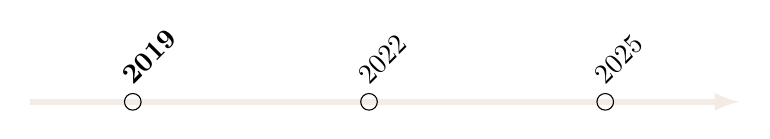
\begin{tikzpicture}[xscale=1]
            \draw[line width=0.7mm,-latex,isgold!20] (0.7,0) -- (9.5+0.2,0);
            \foreach \X [evaluate=\X as \Y using int(\X-2017),count=\Z] in {2022, 2025}
            {
            \draw[highlight on=<0>] (\Y,0) circle[radius=3pt];
            \node[anchor=south,highlight on=<0>,fill=white,rotate=45,anchor=south
            west,inner sep=0pt] at (\Y,0.2) {\X};
            }
            \foreach \X [evaluate=\X as \Y using int(\X-2017),count=\Z] in {2019}
            {
            \draw[highlight on=<\Z>] (\Y,0) circle[radius=3pt];
            \node[anchor=south,highlight on=<\Z>,fill=white,rotate=45,anchor=south
            west,inner sep=0pt] at (\Y,0.2) {\bfseries\X};
            }
        \end{tikzpicture}
    \end{center}
    \vspace{-10pt}
    \begin{columns}[onlytextwidth,t]
        % \column{.01\textwidth}
       \column{.5\textwidth}
       \vspace{-5pt}
       \begin{figure}
            \centering
            \captionsetup{justification=centering}
            % \caption{\texttt{Jet quenching as a probe \\ of the initial stages}}
            \vspace{-5pt}
            \includegraphics[width=1.1\textwidth]{images/raa-vn-tauq_crop.pdf}
        \end{figure}
        \column{.04\textwidth}
        \column{.43\textwidth}
        % \vspace{0.2cm}
        \begin{center}
            \setbeamertemplate{itemize item}{\raisebox{0.1em}{\scalebox{0.5}{${\color{lightgray}\blacktriangleright}$}}}
            {\Large\color{palgold} $R_{AA}$ and $v_2$  \\[10pt]}
            \footnotesize
                \begin{itemize}
                    \item {\color{lightgray}Medium $\rightarrow$ {\bfseries\color{palviolet} EKRT} model + hydro}
                    \item {\color{lightgray}Jet quenching $\rightarrow$ {\bfseries BDMPS-Z}}\\[3pt]
                    {\color{lightgray}Parametrize $\boldsymbol{\hat{q}}\propto K {\color{palviolet}\boldsymbol{\epsilon}}^{3/4}_{\color{palviolet}\mathbf{EKRT}}$, fit $K$ to $R_{AA}$}\\[15pt]
                    \setbeamertemplate{itemize item}{\raisebox{0.2em}{\scalebox{1}{${\color{destacado}\boldsymbol{\Rightarrow}}$}}} 
                    \item {\color{destacado}\bfseries\normalsize{$\boldsymbol{v_2}$ sensitive to pre-hydro stage}}
                    \item {\color{destacado}\bfseries\normalsize{$\boldsymbol{\hat{q}_\mathrm{neq}=0}$ for $\boldsymbol{\tau <0.6\,\mathrm{fm/c}}$}}
                \end{itemize}
                % {\footnotesize\color{lightgray}\texttt{Ballistic diffusion of heavy quarks in \\ the early stage of relativistic heavy \\ ion collisions at RHIC and LHC}}
        \end{center}
        \column{.02\textwidth}
    \end{columns}
    \blfootnote{\scriptsize Andres, Armesto, Niemi, Paatelainen, Salgado \href{https://arxiv.org/abs/1902.03231}{\color{palgold}\texttt{[1902.03231]}$^\text{\scalebox{0.9}{\faExternalLink}}$}\\\hspace{14pt} Eskola, Kajantie, Ruuskanen, Tuominen \href{https://arxiv.org/abs/hep-ph/9909456}{\color{palviolet}\texttt{[hep-ph/9909456]}$^\text{\scalebox{0.9}{\faExternalLink}}$} Niemi, Eskola, Paatelainen \href{https://arxiv.org/abs/1505.02677}{\color{palviolet}\texttt{[1505.02677]}$^\text{\scalebox{0.9}{\faExternalLink}}$}}
\end{frame}

%%%%%%%%%%%%%%%%%%%%%%%%%%%%%%%%%%%%%%%%%
%%%%%%%%%%%%%%%%% SLIDE %%%%%%%%%%%%%%%%%
%%%%%%%%%%%%%%%%%%%%%%%%%%%%%%%%%%%%%%%%%

\begin{frame}[t,noframenumbering]
    \frametitle{Jets in pre-equilibrium}
    \begin{center}
        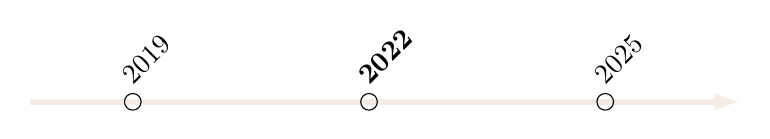
\begin{tikzpicture}[xscale=1]
            \draw[line width=0.7mm,-latex,isgold!20] (0.7,0) -- (9.5+0.2,0);
            \foreach \X [evaluate=\X as \Y using int(\X-2017),count=\Z] in {2019, 2025}
            {
            \draw[highlight on=<0>] (\Y,0) circle[radius=3pt];
            \node[anchor=south,highlight on=<0>,fill=white,rotate=45,anchor=south
            west,inner sep=0pt] at (\Y,0.2) {\X};
            }
            \foreach \X [evaluate=\X as \Y using int(\X-2017),count=\Z] in {2022}
            {
            \draw[highlight on=<\Z>] (\Y,0) circle[radius=3pt];
            \node[anchor=south,highlight on=<\Z>,fill=white,rotate=45,anchor=south
            west,inner sep=0pt] at (\Y,0.2) {\bfseries\X};
            }
        \end{tikzpicture}
    \end{center}
    \vspace{-10pt}
    \begin{columns}[onlytextwidth,t]
        \column{.02\textwidth}
       \column{.47\textwidth}
    %    \vspace{-13pt}
       \begin{figure}
            \centering
            \captionsetup{justification=centering}
            % \caption{\footnotesize\texttt{Medium-induced radiation with vacuum \\ propagation in pre-hydrodynamics phase}}
            \vspace{7pt}
            \includegraphics[width=1.05\textwidth]{images/fig2_v2.pdf}
        \end{figure}
        \column{.02\textwidth}
        \column{.46\textwidth}
        % \vspace{0.2cm}
        \begin{center}
            \setbeamertemplate{itemize item}{\raisebox{0.1em}{\scalebox{0.5}{${\color{lightgray}\blacktriangleright}$}}}
            {\Large\color{isgold} $Q_{AA}$ and $w_2$\\{\scriptsize (proxies for $R_{AA}$ and $v_2$)} \\[10pt]}
            \footnotesize
                \begin{itemize}
                    \item {\color{lightgray}{\bfseries BDMPS-Z} framework for energy loss}
                    % \item {\color{lightgray}Consider {\bfseries vacuum emissions before QGP}}
                    \item {\color{lightgray}Compare {\color{Red}vacuum emissions before QGP}\\ with {\color{OliveGreen}early eloss} and {\color{RoyalBlue}delayed eloss}}
                    % \item {\color{lightgray}Fit $Q_{AA}$, get different $w_2$}
                    \\[15pt]
                    \setbeamertemplate{itemize item}{\raisebox{0.2em}{\scalebox{1}{${\color{destacado}\boldsymbol{\Rightarrow}}$}}} 
                    \item {\color{destacado}\bfseries\normalsize{$\boldsymbol{w_2}$ sensitive to pre-hydro stage}}
                    % \item {\color{lightgray}Extract $Q_{AA}$ and $w_2$, proxies for $R_{AA}$ and $v_2$}
                    % \item {\color{lightgray}Fit $Q_{AA}$, get different $w_2$}
                \end{itemize}
                % {\footnotesize\color{lightgray}\texttt{Ballistic diffusion of heavy quarks in \\ the early stage of relativistic heavy \\ ion collisions at RHIC and LHC}}
        \end{center}
        \column{.02\textwidth}
    \end{columns}
    \blfootnote{\scriptsize Andres, Apolinário, Dominguez, Gonzalez Martinez, Salgado \href{https://arxiv.org/abs/2211.10161}{\color{palgold}\texttt{[2211.10161]}$^\text{\scalebox{0.9}{\faExternalLink}}$}}
\end{frame}



%%%%%%%%%%%%%%%%%%%%%%%%%%%%%%%%%%%%%%%%%
%%%%%%%%%%%%%%%%% SLIDE %%%%%%%%%%%%%%%%%
%%%%%%%%%%%%%%%%%%%%%%%%%%%%%%%%%%%%%%%%%

\begin{frame}[t,noframenumbering]
    \frametitle{Jets in pre-equilibrium}
    \begin{center}
        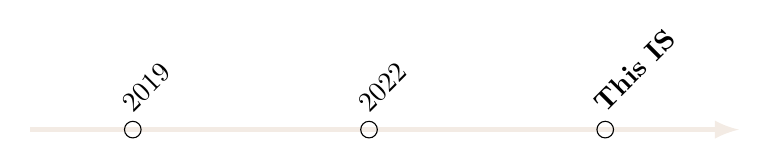
\begin{tikzpicture}[xscale=1]
            \draw[line width=0.7mm,-latex,isgold!20] (0.7,0) -- (9.5+0.2,0);
            \foreach \X [evaluate=\X as \Y using int(\X-2017),count=\Z] in {2019, 2022}
            {
            \draw[highlight on=<0>] (\Y,0) circle[radius=3pt];
            \node[anchor=south,highlight on=<0>,fill=white,rotate=45,anchor=south
            west,inner sep=0pt] at (\Y,0.2) {\X};
            }
            \foreach \X [evaluate=\X as \Y using int(\X-2017),count=\Z] in {2025}
            {
            \draw[highlight on=<\Z>] (\Y,0) circle[radius=3pt];
            \node[anchor=south,highlight on=<\Z>,fill=white,rotate=45,anchor=south
            west,inner sep=0pt] at (\Y,0.2) {\bfseries This IS};
            }
        \end{tikzpicture}
    \end{center}
    \vspace{-10pt}
    \begin{columns}[onlytextwidth,t]
        \column{.02\textwidth}
       \column{.47\textwidth}
    %    \vspace{-13pt}
       \begin{figure}
            \centering
            \captionsetup{justification=centering}
            % \caption{\footnotesize\texttt{Medium-induced radiation with vacuum \\ propagation in pre-hydrodynamics phase}}
            % \vspace{7pt}
            \includegraphics[width=1.05\textwidth]{images/fig3.pdf}
        \end{figure}
        \column{.02\textwidth}
        \column{.46\textwidth}
        % \vspace{0.2cm}
        \begin{center}
            \setbeamertemplate{itemize item}{\raisebox{0.1em}{\scalebox{0.5}{${\color{lightgray}\blacktriangleright}$}}}
            {\Large\color{isgold} $\mathfrak{Q}$ and $\mathfrak{v}_2$\\{\scriptsize (proxies for $R_{AA}$ and $v_2$)} \\[10pt]}
            \footnotesize
                \begin{itemize}
                    \item {\color{lightgray}{\bfseries Improved opacity expansion} for energy loss}
                    \item {\color{lightgray}Model $\hat{q}(t)$ with {\bfseries expansion parameter $\boldsymbol{\alpha}$}}
                    \item {\color{lightgray}{\color{darkqhat}\bfseries Over-occupied} and {\color{lightqhat}\bfseries under-occupied} systems}
                    % \item {\color{lightgray}Extract $\mathfrak{Q}$ and $\mathfrak{v}_2$, proxies for $R_{AA}$ and $v_2$}
                    % \item {\color{lightgray}\bfseries Both $\mathfrak{Q}$ and $\mathfrak{v}_2$ sensitive to $\boldsymbol{\hat{q}}$ model}
                    \\[15pt]
                    \setbeamertemplate{itemize item}{\raisebox{0.2em}{\scalebox{1}{${\color{destacado}\boldsymbol{\Rightarrow}}$}}} 
                    \item {\color{destacado}\bfseries\normalsize{$\mathfrak{Q}$ and $\mathfrak{v}_2$ sensitive to expansion}}
                \end{itemize}
                % {\footnotesize\color{lightgray}\texttt{Ballistic diffusion of heavy quarks in \\ the early stage of relativistic heavy \\ ion collisions at RHIC and LHC}}
        \end{center}
        \column{.02\textwidth}
    \end{columns}
    \blfootnote{\scriptsize Adhya, Tywoniuk \href{https://arxiv.org/abs/2409.04295}{\color{palgold}\texttt{[2409.04295]}$^\text{\scalebox{0.9}{\faExternalLink}}$}}
    \begin{tikzpicture}[overlay, remember picture]
        \node[anchor=north west] 
        at ([xshift=0.05cm,yshift=-0.05cm]current page.north west) {\begin{partalkbox}\scriptsize{\color{destacado}Adhya$\hspace{1pt}^\text{\scalebox{0.9}{\faComment}}$} {\itshape Wed 11:50$\hspace{1pt}^\text{\scalebox{0.9}{\faClockO}}$} \end{partalkbox}};
    \end{tikzpicture}
    \begin{tikzpicture}[overlay, remember picture]
        \node[anchor=north west] 
        at ([xshift=0.05cm,yshift=-0.48cm]current page.north west) {\begin{partalkbox}\scriptsize{\href{https://indico.cern.ch/event/1479384/contributions/6663091/}{{\color{palblue}Jets in early stages$^\text{\scalebox{0.9}{\faHandOLeft}}$}}} \end{partalkbox}};
    \end{tikzpicture}
\end{frame}

%%%%%%%%%%%%%%%%%%%%%%%%%%%%%%%%%%%%%%%%%
%%%%%%%%%%%%%%%%% SLIDE %%%%%%%%%%%%%%%%%
%%%%%%%%%%%%%%%%%%%%%%%%%%%%%%%%%%%%%%%%%

\begin{frame}[t,noframenumbering]
    \frametitle{Jets in pre-equilibrium}
    \framesubtitle{{\footnotesize\color{jyured} (unpublished, ask Adam for better plot)}}
    \begin{center}
        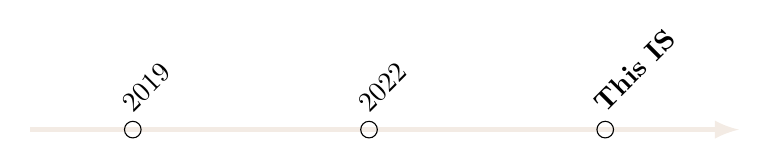
\begin{tikzpicture}[xscale=1]
            \draw[line width=0.7mm,-latex,isgold!20] (0.7,0) -- (9.5+0.2,0);
            \foreach \X [evaluate=\X as \Y using int(\X-2017),count=\Z] in {2019, 2022}
            {
            \draw[highlight on=<0>] (\Y,0) circle[radius=3pt];
            \node[anchor=south,highlight on=<0>,fill=white,rotate=45,anchor=south
            west,inner sep=0pt] at (\Y,0.2) {\X};
            }
            \foreach \X [evaluate=\X as \Y using int(\X-2017),count=\Z] in {2025}
            {
            \draw[highlight on=<\Z>] (\Y,0) circle[radius=3pt];
            \node[anchor=south,highlight on=<\Z>,fill=white,rotate=45,anchor=south
            west,inner sep=0pt] at (\Y,0.2) {\bfseries This IS};
            }
        \end{tikzpicture}
    \end{center}
    \vspace{-10pt}
    \begin{columns}[onlytextwidth,t]
        \column{.02\textwidth}
       \column{.47\textwidth}
    %    \vspace{-13pt}
       \begin{figure}
            \centering
            \captionsetup{justification=centering}
            % \caption{\footnotesize\texttt{Medium-induced radiation with vacuum \\ propagation in pre-hydrodynamics phase}}
            \vspace{-5pt}
            \includegraphics[width=1.05\textwidth]{images/adam_raav2.png}
        \end{figure}
        \column{.02\textwidth}
        \column{.47\textwidth}
        % \vspace{0.2cm}
        \begin{center}
            \setbeamertemplate{itemize item}{\raisebox{0.1em}{\scalebox{0.5}{${\color{lightgray}\blacktriangleright}$}}}
            {\Large\color{isgold} $R_{AA}$ and $v_2$ \\[10pt]}
            \footnotesize
                \begin{itemize}
                    \item {\color{lightgray}Quenching framework with induced radiation}
                    \item {\color{lightgray}Jets in {\bfseries IP-Glasma + MUSIC + UrQMD}}
                    % \item {\color{lightgray}Quenching between $0.1\,\mathrm{fm/c}$ and $0.4\,\mathrm{fm/c}$}
                    \item {\color{lightgray}Extrapolate $\hat{q}$ to early times $0.1-0.4\,\mathrm{fm/c}$\\ using hydrodynamic attractors}\\[15pt]
                    \setbeamertemplate{itemize item}{\raisebox{0.2em}{\scalebox{1}{${\color{destacado}\boldsymbol{\Rightarrow}}$}}} 
                    \item {\color{destacado}\bfseries\normalsize{$\boldsymbol{R_{AA}}$ unaffected, $\boldsymbol{v_2}$ weak sensitivity}}
                    % \item {\color{lightgray}$R_{AA}$ unaffected, $v_2$ weak sensitivity}
                \end{itemize}
                % {\footnotesize\color{lightgray}\texttt{Ballistic diffusion of heavy quarks in \\ the early stage of relativistic heavy \\ ion collisions at RHIC and LHC}}
        \end{center}
        \column{.02\textwidth}
    \end{columns}
    % \blfootnote{\scriptsize Adhya, Tywoniuk \href{https://arxiv.org/abs/2409.04295}{\color{palgold}\texttt{[2409.04295]}$^\text{\scalebox{0.9}{\faExternalLink}}$}}
    \begin{tikzpicture}[overlay, remember picture]
        \node[anchor=north west] 
        at ([xshift=0.05cm,yshift=-0.05cm]current page.north west) {\begin{partalkbox}\scriptsize{\color{destacado}Takacs$\hspace{1pt}^\text{\scalebox{0.9}{\faComment}}$} {\itshape Tue 14:00$\hspace{1pt}^\text{\scalebox{0.9}{\faClockO}}$} \end{partalkbox}};
    \end{tikzpicture}
    \begin{tikzpicture}[overlay, remember picture]
        \node[anchor=north west] 
        at ([xshift=0.05cm,yshift=-0.48cm]current page.north west) {\begin{partalkbox}\scriptsize{\href{https://indico.cern.ch/event/1479384/contributions/6663041/}{{\color{palblue}Jet suppresion and flow$^\text{\scalebox{0.9}{\faHandOLeft}}$}}} \end{partalkbox}};
    \end{tikzpicture}
\end{frame}

%%%%%%%%%%%%%%%%%%%%%%%%%%%%%%%%%%%%%%%%%
%%%%%%%%%%%%%%%%%%%%%%%%%%%%%%%%%%%%%%%%%
%%%%%%%%%%%%%%%%% SLIDE %%%%%%%%%%%%%%%%%
%%%%%%%%%%%%%%%%%%%%%%%%%%%%%%%%%%%%%%%%%

\begin{frame}[plain,noframenumbering]
    \frametitle{}
    \begin{center}
        \begin{figure}
            \smartdiagramset{
                planet color=jyured!10,      
                set color list={isgold!40, palteal!30},
                distance planet-satellite=4.0cm,
                planet size=4cm, 
                planet text width=3.0cm,
                /tikz/connection planet satellite/.append style={<-}
                }
            \smartdiagram[constellation diagram]{
                {\Large\color{jyured}\bfseries No eloss \\ in pre-hydro}, {\Large $R_{AA}$}, {\Large $v_2$} 
            }
        \end{figure}
    \end{center}
\end{frame}

%%%%%%%%%%%%%%%%%%%%%%%%%%%%%%%%%%%%%%%%%
%%%%%%%%%%%%%%%%% SLIDE %%%%%%%%%%%%%%%%%
%%%%%%%%%%%%%%%%%%%%%%%%%%%%%%%%%%%%%%%%%

\begin{frame}[plain,noframenumbering]
    \frametitle{}
    \begin{center}
        \begin{figure}
            \smartdiagramset{
                bubble center node color=jyured!10,      
                set color list={isgold!40, palteal!30, palteal!30, none, none},
                bubble center node size=4.7cm, 
                % planet size=3.5cm,
                % bubble node size=5cm,
                % bubble text width=3.0cm,
                }
            \smartdiagramadd[bubble diagram]{
                {\Large\color{jyured} \textbf{Large} $\boldsymbol{\hat{q}}$ \\ {\Large\color{jyured}\textbf{in glasma}}}, \textit{\footnotesize\color{isgold}Part 1}\\\textbf{\Large\color{isgold} Glasma}, \textit{\color{palteal}Jet} momentum \\ broadening, \textit{\color{palteal}Jet} energy loss, , 
            }{}
            \begin{tikzpicture}[remember picture,overlay]
                \draw[myarrow, draw=isgold!50, line width=2pt, bend right=15]
                (module2) to (module3);
                % \draw[myarrow, draw=isgold!50, line width=2pt, bend left=15]
                % (module2) to (module6);
                \draw[myleftrightarrow, draw=palteal!50, bend right=15]
                (module3) to (module4);
                % \draw[myarrow, draw=palteal!70, bend right=15]
                % (module3) to (module4);
                % \draw[myarrow, draw=palteal!70, bend left=15]
                % (module4) to (module3);
                % \draw[myarrow, draw=palviolet, line width=2pt, bend left=20, dashed]
                % (module2) to (module6);
            \end{tikzpicture}

            % \smartdiagramconnect{{-latex},palteal,line width=2pt,bend left=20}{module2/module3}
            % \smartdiagramconnect{<-}{module3/module2}
        \end{figure}
    \end{center}
\end{frame}

% %%%%%%%%%%%%%%%%%%%%%%%%%%%%%%%%%%%%%%%%%
% %%%%%%%%%%%%%%%%% SLIDE %%%%%%%%%%%%%%%%%
% %%%%%%%%%%%%%%%%%%%%%%%%%%%%%%%%%%%%%%%%%

% \begin{frame}[plain,noframenumbering]
%     \frametitle{\\From classical broadening...}
%     \vspace{10pt}
%     \begin{center}
%         \includegraphics[height=0.7\paperheight]{images/momentum_broadening_flipped_cljet.png}
%     \end{center}
% \end{frame}

% %%%%%%%%%%%%%%%%%%%%%%%%%%%%%%%%%%%%%%%%%
% %%%%%%%%%%%%%%%%% SLIDE %%%%%%%%%%%%%%%%%
% %%%%%%%%%%%%%%%%%%%%%%%%%%%%%%%%%%%%%%%%%

% \begin{frame}[plain,noframenumbering]
%     \frametitle{\\...to radiation in glasma fields}
%     \vspace{10pt}
%     \begin{center}
%         \includegraphics[height=0.7\paperheight]{images/momentum_broadening_flipped_jetquenched.png}
%     \end{center}
% \end{frame}

% %%%%%%%%%%%%%%%%%%%%%%%%%%%%%%%%%%%%%%%%%
% %%%%%%%%%%%%%%%%% SLIDE %%%%%%%%%%%%%%%%%
% %%%%%%%%%%%%%%%%%%%%%%%%%%%%%%%%%%%%%%%%%

% \begin{frame}
%     \frametitle{Jet quenching in glasma}
%     % \framesubtitle{Synchrotron radiation in color domains}
%     \vspace{-15pt}
%     \begin{center}
%         \begin{columns}[onlytextwidth,t]
%             \column{.02\textwidth}
%            \column{.4\textwidth}
%             \vspace{5pt}
%             \begin{center}
%                 \includegraphics[width=0.88\columnwidth]{images/target_domains.pdf}
%                 \\[5pt]
%                 \includegraphics[width=0.88\columnwidth]{images/glasma_corr_dom_jet.pdf}
%             \end{center}

%             \column{.02\textwidth}
%             \column{.54\textwidth}
%             \begin{center}
%                 \begin{custombox2}{\normalsize Color domains}{raablue}
%                     \small
%                     \begin{varwidth}{0.89\textwidth}
%                     \begin{itemize}\itemsep0em 
%                         \itemsep0em
%                         \footnotesize
%                         \setbeamertemplate{itemize item}{\raisebox{0.2em}{\scalebox{0.7}{${\color{raablue}\blacktriangleright}$}}} 
%                         \item Consecutive color {\bfseries\color{raablue}longitudinal electric fields}
%                         \item Fields constant in {\bfseries\color{jyured}color domains $\boldsymbol{l\sim 1/Q_s}$}
%                         \item {\bfseries\color{raablue} Gaussian averages} over the electric fields
%                     \end{itemize}
%                     \end{varwidth}
%                 \end{custombox2}
%                 % \begin{custombox2}{\normalsize BDMPS-Z style calculation}{palviolet}
%                 %     \small
%                 %     \begin{varwidth}{0.89\textwidth}
%                 %     \begin{itemize}\itemsep0em 
%                 %         \itemsep0em
%                 %         \footnotesize
%                 %         \setbeamertemplate{itemize item}{\raisebox{0.2em}{\scalebox{0.7}{${\color{palviolet}\blacktriangleright}$}}} 
%                 %         \item Medium averages $\neq$ simple factorization
%                 %         \item Extract jet quenching parameter $\boldsymbol{\hat{q}}$ and \\{\bfseries\color{palviolet} rate of medium-induced radiation $\boldsymbol{\mathrm{d}\Gamma/\mathrm{d}x}$}
%                 %         \item {\bfseries\color{raablue}Single tube} $\sim$ synchrotron radiation 
%                 %         \item {\bfseries\color{raablue}Multiple tubes} $\Rightarrow$ rate decreases
%                 %     \end{itemize}
%                 %     \end{varwidth}
%                 % \end{custombox2}
%             \end{center}
%             \vspace{-10pt}
%             % \begin{figure}
%             %     \centering
%             %     \includegraphics[width=0.95\columnwidth]{images/tblfq_sectors_onlyq.png}
%             % \end{figure}
%             \column{.02\textwidth}
%         \end{columns}    
%     \end{center}
%     \vspace{-10pt}
%     \blfootnote{\scriptsize Barata, Hauksson, López, Sadofyev \href{https://arxiv.org/abs/2406.07615}{{\color{raablue}\texttt{[2406.07615]$^\text{\scalebox{0.9}{\faExternalLink}}$}}}  Agostini, Altinoluk, Armesto \href{https://arxiv.org/abs/2103.08485}{{\color{raapink}\texttt{[2103.08485]$^\text{\scalebox{0.9}{\faExternalLink}}$}}}}
%     \begin{tikzpicture}[overlay, remember picture]
%         \node[anchor=north west] 
%         at ([xshift=0.05cm,yshift=-0.05cm]current page.north west) {\begin{plentalkbox}\scriptsize{\color{destacado}Sadofyev$\hspace{1pt}^\text{\scalebox{0.9}{\faComment}}$} {\itshape Thu 16:50$\hspace{1pt}^\text{\scalebox{0.9}{\faClockO}}$} \end{plentalkbox}};
%     \end{tikzpicture}
%     \begin{tikzpicture}[overlay, remember picture]
%         \node[anchor=north west] 
%         at ([xshift=0.05cm,yshift=-0.48cm]current page.north west) {\begin{plentalkbox}\scriptsize{\href{https://indico.cern.ch/event/1479384/contributions/6632069/}{{\color{isgold}Jet quenching in glasma$^\text{\scalebox{0.9}{\faHandOLeft}}$}}} \end{plentalkbox}};
%     \end{tikzpicture}
% \end{frame}


% %%%%%%%%%%%%%%%%%%%%%%%%%%%%%%%%%%%%%%%%%
% %%%%%%%%%%%%%%%%% SLIDE %%%%%%%%%%%%%%%%%
% %%%%%%%%%%%%%%%%%%%%%%%%%%%%%%%%%%%%%%%%%

% \begin{frame}[noframenumbering]
%     \frametitle{Jet quenching in glasma}
%     % \framesubtitle{Synchrotron radiation in color domains}
%     \vspace{-15pt}
%     \begin{center}
%         \begin{columns}[onlytextwidth,t]
%             \column{.02\textwidth}
%            \column{.4\textwidth}
%             \vspace{5pt}
%             \begin{center}
%                 \includegraphics[width=0.88\columnwidth]{images/glasma_corr_dom_jet.pdf}
%                 \\[5pt]
%                 % \includegraphics[width=0.9\columnwidth]{images/su2manyall.pdf}
%                 \includegraphics[width=0.95\columnwidth]{images/jeteloss.pdf}
%             \end{center}

%             \column{.02\textwidth}
%             \column{.54\textwidth}
%             \begin{center}
%                 \begin{custombox2}{\normalsize Color domains}{raablue}
%                     \small
%                     \begin{varwidth}{0.89\textwidth}
%                     \begin{itemize}\itemsep0em 
%                         \itemsep0em
%                         \footnotesize
%                         \setbeamertemplate{itemize item}{\raisebox{0.2em}{\scalebox{0.7}{${\color{raablue}\blacktriangleright}$}}} 
%                         \item Consecutive color {\bfseries\color{raablue}longitudinal electric fields}
%                         \item Fields constant in {\bfseries\color{jyured}color domains $\boldsymbol{l\sim 1/Q_s}$}
%                         \item {\bfseries\color{raablue} Gaussian averages} over the electric fields
%                     \end{itemize}
%                     \end{varwidth}
%                 \end{custombox2}
%                 \begin{custombox2}{\normalsize BDMPS-Z style calculation}{palviolet}
%                     \small
%                     \begin{varwidth}{0.89\textwidth}
%                     \begin{itemize}\itemsep0em 
%                         \itemsep0em
%                         \footnotesize
%                         \setbeamertemplate{itemize item}{\raisebox{0.2em}{\scalebox{0.7}{${\color{palviolet}\blacktriangleright}$}}} 
%                         \item Medium averages $\neq$ simple factorization
%                         \item Extract jet quenching parameter $\boldsymbol{\hat{q}}$ and \\{\bfseries\color{palviolet} rate of medium-induced radiation $\boldsymbol{\mathrm{d}\Gamma/\mathrm{d}x}$}
%                          \setbeamertemplate{itemize item}{\raisebox{0.2em}{\scalebox{0.7}{${\color{raablue}\blacktriangleright}$}}} 
%                         \item {\bfseries\color{raablue}Single tube} $\sim$ synchrotron radiation 
%                         \item {\bfseries\color{raablue}Multiple tubes} $\Rightarrow$ rate decreases
%                     \end{itemize}
%                     \end{varwidth}
%                 \end{custombox2}
%             \end{center}
%             \vspace{-10pt}
%             % \begin{figure}
%             %     \centering
%             %     \includegraphics[width=0.95\columnwidth]{images/tblfq_sectors_onlyq.png}
%             % \end{figure}
%             \column{.02\textwidth}
%         \end{columns}    
%     \end{center}
%     \vspace{-10pt}
%     \blfootnote{\scriptsize Barata, Hauksson, López, Sadofyev \href{https://arxiv.org/abs/2406.07615}{{\color{raablue}\texttt{[2406.07615]$^\text{\scalebox{0.9}{\faExternalLink}}$}}}}
%     \begin{tikzpicture}[overlay, remember picture]
%         \node[anchor=north west] 
%         at ([xshift=0.05cm,yshift=-0.05cm]current page.north west) {\begin{plentalkbox}\scriptsize{\color{destacado}Sadofyev$\hspace{1pt}^\text{\scalebox{0.9}{\faComment}}$} {\itshape Thu 16:50$\hspace{1pt}^\text{\scalebox{0.9}{\faClockO}}$} \end{plentalkbox}};
%     \end{tikzpicture}
%     \begin{tikzpicture}[overlay, remember picture]
%         \node[anchor=north west] 
%         at ([xshift=0.05cm,yshift=-0.48cm]current page.north west) {\begin{plentalkbox}\scriptsize{\href{https://indico.cern.ch/event/1479384/contributions/6632069/}{{\color{isgold}Jet quenching in glasma$^\text{\scalebox{0.9}{\faHandOLeft}}$}}} \end{plentalkbox}};
%     \end{tikzpicture}
% \end{frame}

% %%%%%%%%%%%%%%%%%%%%%%%%%%%%%%%%%%%%%%%%%
% %%%%%%%%%%%%%%%%% SLIDE %%%%%%%%%%%%%%%%%
% %%%%%%%%%%%%%%%%%%%%%%%%%%%%%%%%%%%%%%%%%

% \begin{frame}
%     \frametitle{Quantum jets}
%     % \framesubtitle{In classical glasma fields}
%     \vspace{-15pt}
%     \begin{center}
%         \begin{columns}[onlytextwidth,t]
%             \column{.02\textwidth}
%            \column{.4\textwidth}
%            \begin{center}
                
%                 % \begin{untitledcustombox}
%                 %     \begin{varwidth}{0.88\textwidth}
%                 %         \hspace{10pt}\normalsize{\bfseries\color{palteal} This study}: FONLL + {\color{palteal}EPPS16}\hspace{10pt}
%                 %     \end{varwidth}
%                 % \end{untitledcustombox}
%             \end{center}

%             \vspace{-10pt}
%             \begin{center}
%                 \includegraphics[width=0.88\columnwidth]{images/qA_worldline_mono.pdf}
%             \end{center}

%             \column{.02\textwidth}
%             \column{.54\textwidth}
%             \begin{center}
%                 \begin{custombox2}{\normalsize tBLFQ approach}{raablue}
%                     \small
%                     \begin{varwidth}{0.91\textwidth}
%                     \begin{itemize}\itemsep0em 
%                         \itemsep0em
%                         \footnotesize
%                         \setbeamertemplate{itemize item}{\raisebox{0.2em}{\scalebox{0.7}{${\color{raablue}\blacktriangleright}$}}} 
%                         \item Time-dependent basis light-front quantization
%                     \end{itemize}
%                     \end{varwidth}
%                 \end{custombox2}
%                 \begin{custombox2}{\normalsize Quantum jets in classical fields}{raapink}
%                     \small
%                     \begin{varwidth}{0.91\textwidth}
%                     \begin{itemize}\itemsep0em 
%                         \itemsep0em
%                         \footnotesize
%                         \setbeamertemplate{itemize item}{\raisebox{0.2em}{\scalebox{0.7}{${\color{raapink}\blacktriangleright}$}}} 
%                         \item Schr\"{o}dinger equation for jet evolution using {\bfseries\color{raapink} light-front quantization of QCD}
%                         \item Interaction term with classical gluon field $\mathcal{A}$
%                     \end{itemize}
%                     \end{varwidth}
%                 \end{custombox2}
%             \end{center}
%             \vspace{-10pt}
%             \begin{figure}
%                 \centering
%                 \includegraphics[width=0.95\columnwidth]{images/tblfq_sectors_onlyq.png}
%             \end{figure}
%             \column{.02\textwidth}
%         \end{columns}    
%     \end{center}
%     \vspace{-10pt}
%     \blfootnote{\scriptsize Li, Zhao, Maris, Chen, Li, Tuchin, Vary \href{https://arxiv.org/abs/2002.09757}{{\color{raablue}\texttt{[2002.09757]$^\text{\scalebox{0.9}{\faExternalLink}}$}}} Li, Lappi, Zhao, Salgado \href{https://arxiv.org/abs/2305.12490}{{\color{raablue}\texttt{[2305.12490]$^\text{\scalebox{0.9}{\faExternalLink}}$}}}}
%     \begin{tikzpicture}[overlay, remember picture]
%         \node[anchor=north west] 
%         at ([xshift=0.05cm,yshift=-0.05cm]current page.north west) {\begin{partalkbox}\scriptsize{\color{destacado}Li$\hspace{1pt}^\text{\scalebox{0.9}{\faComment}}$} {\itshape Wed 9:20$\hspace{1pt}^\text{\scalebox{0.9}{\faClockO}}$} \end{partalkbox}};
%     \end{tikzpicture}
%     \begin{tikzpicture}[overlay, remember picture]
%         \node[anchor=north west] 
%         at ([xshift=0.05cm,yshift=-0.48cm]current page.north west) {\begin{partalkbox}\scriptsize{\href{https://indico.cern.ch/event/1479384/contributions/6663075/}{{\color{palblue}Quantum jets in colored fields$^\text{\scalebox{0.9}{\faHandOLeft}}$}}} \end{partalkbox}};
%     \end{tikzpicture}
% \end{frame}

% %%%%%%%%%%%%%%%%%%%%%%%%%%%%%%%%%%%%%%%%%
% %%%%%%%%%%%%%%%%% SLIDE %%%%%%%%%%%%%%%%%
% %%%%%%%%%%%%%%%%%%%%%%%%%%%%%%%%%%%%%%%%%

% \begin{frame}
%     \frametitle{Quantum gluon emission}
%     % \framesubtitle{In classical glasma fields}
%     \vspace{-15pt}
%     \begin{center}
%         \begin{columns}[onlytextwidth,t]
%             \column{.02\textwidth}
%            \column{.4\textwidth}
%            \begin{center}
                
%                 % \begin{untitledcustombox}
%                 %     \begin{varwidth}{0.88\textwidth}
%                 %         \hspace{10pt}\normalsize{\bfseries\color{palteal} This study}: FONLL + {\color{palteal}EPPS16}\hspace{10pt}
%                 %     \end{varwidth}
%                 % \end{untitledcustombox}
%             \end{center}

%             \vspace{-10pt}
%             \begin{center}
%                 \includegraphics[width=0.88\columnwidth]{images/F1_qgA_worldline_mono.pdf}
%             \end{center}

%             \column{.02\textwidth}
%             \column{.54\textwidth}
%             \begin{center}
%                 \begin{custombox2}{\normalsize tBLFQ approach}{raablue}
%                     \small
%                     \begin{varwidth}{0.91\textwidth}
%                     \begin{itemize}\itemsep0em 
%                         \itemsep0em
%                         \footnotesize
%                         \setbeamertemplate{itemize item}{\raisebox{0.2em}{\scalebox{0.7}{${\color{raablue}\blacktriangleright}$}}} 
%                         \item Time-dependent basis light-front quantization
%                     \end{itemize}
%                     \end{varwidth}
%                 \end{custombox2}
%                 \begin{custombox2}{\normalsize Quantum jets in classical fields}{raapink}
%                     \small
%                     \begin{varwidth}{0.91\textwidth}
%                     \begin{itemize}\itemsep0em 
%                         \itemsep0em
%                         \footnotesize
%                         \setbeamertemplate{itemize item}{\raisebox{0.2em}{\scalebox{0.7}{${\color{raapink}\blacktriangleright}$}}} 
%                         \item Schr\"{o}dinger equation for jet evolution using {\bfseries\color{raapink} light-front quantization of QCD}
%                         \item Interaction term with classical gluon field $\mathcal{A}$
%                     \end{itemize}
%                     \end{varwidth}
%                 \end{custombox2}
%             \end{center}
%             \vspace{-10pt}
%             \begin{figure}
%                 \centering
%                 \includegraphics[width=0.95\columnwidth]{images/tblfq_sectors.png}
%             \end{figure}
%             \column{.02\textwidth}
%         \end{columns}    
%     \end{center}
%     \vspace{-10pt}
%     \blfootnote{\scriptsize Li, Zhao, Maris, Chen, Li, Tuchin, Vary \href{https://arxiv.org/abs/2002.09757}{{\color{raablue}\texttt{[2002.09757]$^\text{\scalebox{0.9}{\faExternalLink}}$}}} Li, Lappi, Zhao, Salgado \href{https://arxiv.org/abs/2305.12490}{{\color{raablue}\texttt{[2305.12490]$^\text{\scalebox{0.9}{\faExternalLink}}$}}}}
%     \begin{tikzpicture}[overlay, remember picture]
%         \node[anchor=north west] 
%         at ([xshift=0.05cm,yshift=-0.05cm]current page.north west) {\begin{partalkbox}\scriptsize{\color{destacado}Li$\hspace{1pt}^\text{\scalebox{0.9}{\faComment}}$} {\itshape Wed 9:20$\hspace{1pt}^\text{\scalebox{0.9}{\faClockO}}$} \end{partalkbox}};
%     \end{tikzpicture}
%     \begin{tikzpicture}[overlay, remember picture]
%         \node[anchor=north west] 
%         at ([xshift=0.05cm,yshift=-0.48cm]current page.north west) {\begin{partalkbox}\scriptsize{\href{https://indico.cern.ch/event/1479384/contributions/6663075/}{{\color{palblue}Quantum jets in colored fields$^\text{\scalebox{0.9}{\faHandOLeft}}$}}} \end{partalkbox}};
%     \end{tikzpicture}
% \end{frame}


% %%%%%%%%%%%%%%%%%%%%%%%%%%%%%%%%%%%%%%%%%
% %%%%%%%%%%%%%%%%% SLIDE %%%%%%%%%%%%%%%%%
% %%%%%%%%%%%%%%%%%%%%%%%%%%%%%%%%%%%%%%%%%

% \begin{frame}[noframenumbering]
%     \frametitle{Quantum jets in glasma}
%     % \framesubtitle{In classical glasma fields}
%     \vspace{-15pt}
%     \begin{center}
%         \begin{columns}[onlytextwidth,t]
%             \column{.02\textwidth}
%            \column{.4\textwidth}
%            \begin{center}
                
%                 % \begin{untitledcustombox}
%                 %     \begin{varwidth}{0.88\textwidth}
%                 %         \hspace{10pt}\normalsize{\bfseries\color{palteal} This study}: FONLL + {\color{palteal}EPPS16}\hspace{10pt}
%                 %     \end{varwidth}
%                 % \end{untitledcustombox}
%             \end{center}

%             % \vspace{-10pt}
%             \begin{center}
%                 \includegraphics[width=0.88\columnwidth]{images/quantummombroad.pdf}
%             \end{center}

%             \column{.02\textwidth}
%             \column{.54\textwidth}
%             \begin{center}
%                 % \begin{custombox2}{\normalsize tBLFQ approach}{raablue}
%                 %     \small
%                 %     \begin{varwidth}{0.91\textwidth}
%                 %     \begin{itemize}\itemsep0em 
%                 %         \itemsep0em
%                 %         \footnotesize
%                 %         \setbeamertemplate{itemize item}{\raisebox{0.2em}{\scalebox{0.7}{${\color{raablue}\blacktriangleright}$}}} 
%                 %         \item Time-dependent basis light-front quantization
%                 %     \end{itemize}
%                 %     \end{varwidth}
%                 % \end{custombox2}
%                 \begin{custombox2}{\normalsize Quantum jets in glasma}{raapink}
%                     \small
%                     \begin{varwidth}{0.92\textwidth}
%                     \begin{itemize}\itemsep0em 
%                         \itemsep0em
%                         \footnotesize
%                         \setbeamertemplate{itemize item}{\raisebox{0.2em}{\scalebox{0.7}{${\color{raapink}\blacktriangleright}$}}} 
%                         \item Schr\"{o}dinger equation for {\bfseries\color{raapink} quark state $\boldsymbol{|\psi; x^+\rangle}$} evolved with Hamitonian $P^-$
%                         \item Light-front Hamiltonian $P^-$ in {\bfseries\color{jyured}eikonal limit}\\ picks only
%                         ${\color{jyured}\boldsymbol{\mathcal{A}_+}}$
%                         \item Glasma field $\mathcal{A}$ as numerical solution to CYM 
%                     \end{itemize}
%                     \end{varwidth}
%                 \end{custombox2}
%                 \begin{custombox2}{\normalsize Canonic momentum broadening}{raablue}
%                     \small
%                     \begin{varwidth}{0.8\textwidth}
%                     \begin{itemize}\itemsep0em 
%                         \itemsep0em
%                         \footnotesize
%                         \setbeamertemplate{itemize item}{\raisebox{0.2em}{\scalebox{0.7}{${\color{raablue}\blacktriangleright}$}}} 
%                         \item Quantum $\langle p_i^2(x^+) \rangle=\langle \psi;x^+|p_i^2|\psi;x^+\rangle$
%                         \item Classical from Wong's equations 
%                     \end{itemize}
%                     \end{varwidth}
%                 \end{custombox2}
%             \end{center}
%             % \vspace{-10pt}
%             % \begin{figure}
%             %     \centering
%             %     \includegraphics[width=0.95\columnwidth]{images/tblfq_sectors.png}
%             % \end{figure}
            
%             \column{.02\textwidth}
%         \end{columns}    
%     \end{center}
%     \vspace{-10pt}
%     \blfootnote{\scriptsize \textbf{DA}, Lamas, Lappi, Li, Salgado \href{https://arxiv.org/abs/2506.06206}{{\color{raablue}\texttt{[2506.06206]$^\text{\scalebox{0.9}{\faExternalLink}}$}}}}
%     \begin{tikzpicture}[overlay, remember picture]
%         \node[anchor=north west] 
%         at ([xshift=0.05cm,yshift=-0.05cm]current page.north west) {\begin{partalkbox}\scriptsize{\color{destacado}Lamas$\hspace{1pt}^\text{\scalebox{0.9}{\faComment}}$} {\itshape Wed 11:10$\hspace{1pt}^\text{\scalebox{0.9}{\faClockO}}$} \end{partalkbox}};
%     \end{tikzpicture}
%     \begin{tikzpicture}[overlay, remember picture]
%         \node[anchor=north west] 
%         at ([xshift=0.05cm,yshift=-0.48cm]current page.north west) {\begin{partalkbox}\scriptsize{\href{https://indico.cern.ch/event/1479384/contributions/6663089/}{{\color{palblue}Quantum jets in glasma$^\text{\scalebox{0.9}{\faHandOLeft}}$}}} \end{partalkbox}};
%     \end{tikzpicture}
% \end{frame}

% %%%%%%%%%%%%%%%%%%%%%%%%%%%%%%%%%%%%%%%%%
% %%%%%%%%%%%%%%%%% SLIDE %%%%%%%%%%%%%%%%%
% %%%%%%%%%%%%%%%%%%%%%%%%%%%%%%%%%%%%%%%%%

% \begin{frame}[plain,noframenumbering]
%     \frametitle{}
%     \begin{center}
%         \begin{figure}
%             \smartdiagramset{
%                 bubble center node color=gray!10,      
%                 set color list={isgold!40, none, none, none, palviolet!30}
%                 }
%             \smartdiagramadd[bubble diagram]{
%                 {\color{destacado}\textit{Hard probes} \\ in \textbf{pre-equilibrium}}, \textit{\footnotesize\color{isgold}Part 1}\\\textbf{\Large\color{isgold} Glasma}, , , , \textit{\color{palviolet}Heavy quark}\\ diffusion
%             }{}
%             \begin{tikzpicture}[remember picture,overlay]
%                 \draw[myarrow, draw=isgold!50, line width=2pt, bend left=15]
%                 (module2) to (module6);
%             \end{tikzpicture}
%         \end{figure}
%     \end{center}
% \end{frame}


% %%%%%%%%%%%%%%%%%%%%%%%%%%%%%%%%%%%%%%%%%
% %%%%%%%%%%%%%%%%% SLIDE %%%%%%%%%%%%%%%%%
% %%%%%%%%%%%%%%%%%%%%%%%%%%%%%%%%%%%%%%%%%

% \begin{frame}[t]
%     \frametitle{Heavy quakrs in glasma}
%     \begin{center}
%         \begin{tikzpicture}[xscale=1]
%             \draw[line width=0.7mm,-latex,isgold!20] (-0.2,0) -- (7.5+0.2,0);
%             \foreach \X [evaluate=\X as \Y using int(\X-2018),count=\Z] in {2021, 2024}
%             {
%             \draw[highlight on=<0>] (\Y,0) circle[radius=3pt];
%             \node[anchor=south,highlight on=<0>,fill=white,rotate=45,anchor=south
%             west,inner sep=0pt] at (\Y,0.2) {\X};
%             }
%             \foreach \X [evaluate=\X as \Y using int(\X-2018),count=\Z] in {2019}
%             {
%             \draw[highlight on=<\Z>] (\Y,0) circle[radius=3pt];
%             \node[anchor=south,highlight on=<\Z>,fill=white,rotate=45,anchor=south
%             west,inner sep=0pt] at (\Y,0.2) {\bfseries\X};
%             }
%         \end{tikzpicture}
%     \end{center}
%     \vspace{-10pt}
%     \begin{columns}[onlytextwidth,t]
%         \column{.02\textwidth}
%        \column{.43\textwidth}
%     %    \vspace{-13pt}
%        \begin{figure}
%             \centering
%             \captionsetup{justification=centering}
%             % \caption{\texttt{Impact of Glasma on heavy quark \\ observables in AA collisions}}
%             % \vspace{-5pt}
%             \includegraphics[width=0.95\textwidth]{images/1-s2.0-S0370269319306550-gr003_lrg.jpg}
%         \end{figure}
%         \column{.02\textwidth}
%         \column{.5\textwidth}
%         % \vspace{0.2cm}
%         \begin{center}
%             \setbeamertemplate{itemize item}{\raisebox{0.1em}{\scalebox{0.5}{${\color{lightgray}\blacktriangleright}$}}}
%             {\Large\color{isgold} $R_{AA}$ and $v_2$ for D-mesons \\[10pt]}
%             \footnotesize
%                 \begin{itemize}
%                     \item {\color{lightgray}Numerical glasma fields $\rightarrow$ CYM}
%                     \item {\color{lightgray}Numerical heavy quarks $\rightarrow$ Wong}
%                     \item {\color{lightgray}Coupled to {\bfseries Langevin with drag and diffusion}}\\[15pt]
%                     \setbeamertemplate{itemize item}{\raisebox{0.2em}{\scalebox{1}{${\color{destacado}\boldsymbol{\Rightarrow}}$}}} 
%                     \item {\color{destacado}\bfseries\normalsize{Broadening in glasma increases $\boldsymbol{v_2}$}}
%                 \end{itemize}
%                 % {\footnotesize\color{lightgray}\texttt{Ballistic diffusion of heavy quarks in \\ the early stage of relativistic heavy \\ ion collisions at RHIC and LHC}}
%         \end{center}
%         \column{.02\textwidth}
%     \end{columns}
%     \blfootnote{\scriptsize Sun, Coci, Das, Plumari, Ruggieri, Greco \href{https://arxiv.org/abs/1902.06254}{\color{palgold}\texttt{[1902.06254]}$^\text{\scalebox{0.9}{\faExternalLink}}$}}
% \end{frame}


% %%%%%%%%%%%%%%%%%%%%%%%%%%%%%%%%%%%%%%%%%
% %%%%%%%%%%%%%%%%% SLIDE %%%%%%%%%%%%%%%%%
% %%%%%%%%%%%%%%%%%%%%%%%%%%%%%%%%%%%%%%%%%

% \begin{frame}[t,noframenumbering]
%     \frametitle{Heavy quakrs in glasma}
%     \begin{center}
%         \begin{tikzpicture}[xscale=1]
%             \draw[line width=0.7mm,-latex,isgold!20] (-0.2,0) -- (7.5+0.2,0);
%             \foreach \X [evaluate=\X as \Y using int(\X-2018),count=\Z] in {2019, 2024}
%             {
%             \draw[highlight on=<0>] (\Y,0) circle[radius=3pt];
%             \node[anchor=south,highlight on=<0>,fill=white,rotate=45,anchor=south
%             west,inner sep=0pt] at (\Y,0.2) {\X};
%             }
%             \foreach \X [evaluate=\X as \Y using int(\X-2018),count=\Z] in {2021}
%             {
%             \draw[highlight on=<\Z>] (\Y,0) circle[radius=3pt];
%             \node[anchor=south,highlight on=<\Z>,fill=white,rotate=45,anchor=south
%             west,inner sep=0pt] at (\Y,0.2) {\bfseries\X};
%             }
%         \end{tikzpicture}
%     \end{center}
%     \vspace{-10pt}
%     \begin{columns}[onlytextwidth,t]
%         \column{.02\textwidth}
%        \column{.42\textwidth}
%     %    \vspace{-13pt}
%        \begin{figure}
%             \centering
%             \captionsetup{justification=centering}
%             % \caption{\texttt{Heavy quarks in the early \\ stage of high energy collisions
%             % }}
%             \vspace{-15pt}
%             \includegraphics[width=0.95\textwidth]{images/spcharm.png}
%         \end{figure}
%         \column{.02\textwidth}
%         \column{.52\textwidth}
%         % \vspace{0.2cm}
%         \begin{center}
%             \setbeamertemplate{itemize item}{\raisebox{0.1em}{\scalebox{0.5}{${\color{lightgray}\blacktriangleright}$}}}
%             {\Large\color{isgold} Momentum variance $\sigma_p$ \\[10pt]}
%             \footnotesize
%                 \begin{itemize}
%                     \item {\color{lightgray}Numerical glasma fields $\rightarrow$ CYM}
%                     \item {\color{lightgray}Numerical heavy quarks $\rightarrow$ Wong}
%                     \item {\color{lightgray}Dynamics compared to {\bfseries pQCD Langevin}}\\[15pt]
%                     \setbeamertemplate{itemize item}{\raisebox{0.2em}{\scalebox{1}{${\color{destacado}\boldsymbol{\Rightarrow}}$}}} 
%                     \item {\color{destacado}\bfseries\normalsize{Transport in glasma $\boldsymbol{\neq}$ {\bfseries brownian motion}}}
%                 \end{itemize}
%                 % {\footnotesize\color{lightgray}\texttt{Ballistic diffusion of heavy quarks in \\ the early stage of relativistic heavy \\ ion collisions at RHIC and LHC}}
%         \end{center}
%         \column{.02\textwidth}
%     \end{columns}
%     \blfootnote{\scriptsize Pooja, Das, Oliva, Ruggieri \href{https://arxiv.org/abs/2110.14610}{\color{palgold}\texttt{[2110.14610]}$^\text{\scalebox{0.9}{\faExternalLink}}$}}
%     % \begin{tikzpicture}[overlay, remember picture]
%     %     \node[anchor=north west] 
%     %     at ([xshift=0.05cm,yshift=-0.05cm]current page.north west) {\begin{talkbox}\scriptsize{\color{destacado}Ruggieri$\hspace{1pt}^\text{\scalebox{0.9}{\faComment}}$} {\itshape Mon 11:00$\hspace{1pt}^\text{\scalebox{0.9}{\faClockO}}$} \end{talkbox}};
%     % \end{tikzpicture}
% \end{frame}

% %%%%%%%%%%%%%%%%%%%%%%%%%%%%%%%%%%%%%%%%%
% %%%%%%%%%%%%%%%%% SLIDE %%%%%%%%%%%%%%%%%
% %%%%%%%%%%%%%%%%%%%%%%%%%%%%%%%%%%%%%%%%%

% \begin{frame}[t,noframenumbering]
%     \frametitle{Heavy quakrs in glasma}
%     \begin{center}
%         \begin{tikzpicture}[xscale=1]
%             \draw[line width=0.7mm,-latex,isgold!20] (-0.2,0) -- (7.5+0.2,0);
%             \foreach \X [evaluate=\X as \Y using int(\X-2018),count=\Z] in {2019, 2021}
%             {
%             \draw[highlight on=<0>] (\Y,0) circle[radius=3pt];
%             \node[anchor=south,highlight on=<0>,fill=white,rotate=45,anchor=south
%             west,inner sep=0pt] at (\Y,0.2) {\X};
%             }
%             \foreach \X [evaluate=\X as \Y using int(\X-2018),count=\Z] in {2024}
%             {
%             \draw[highlight on=<\Z>] (\Y,0) circle[radius=3pt];
%             \node[anchor=south,highlight on=<\Z>,fill=white,rotate=45,anchor=south
%             west,inner sep=0pt] at (\Y,0.2) {\bfseries\X};
%             }
%         \end{tikzpicture}
%     \end{center}
%     \vspace{-10pt}
%     \begin{columns}[onlytextwidth,t]
%         \column{.02\textwidth}
%        \column{.44\textwidth}
%     %    \vspace{-13pt}
%        \begin{figure}
%             \centering
%             \captionsetup{justification=centering}
%             % \caption{\texttt{Heavy quarks in the early \\ stage of high energy collisions
%             % }}
%             \vspace{-5pt}
%             \includegraphics[width=0.7\textwidth]{images/Compare_Dissociation_vs_t_Singlet_Triplet_c.pdf}
%         \end{figure}
%         \column{.02\textwidth}
%         \column{.5\textwidth}
%         % \vspace{0.2cm}
%         \begin{center}
%             \setbeamertemplate{itemize item}{\raisebox{0.1em}{\scalebox{0.5}{${\color{lightgray}\blacktriangleright}$}}}
%             {\Large\color{isgold} Dissociation of $c\overline{c}$ and $b\overline{b}$ \\[10pt]}
%             \footnotesize
%                 \begin{itemize}
%                     \item {\color{lightgray}Numerical glasma fields $\rightarrow$ CYM}
%                     \item {\color{lightgray}Numerical heavy quarks $\rightarrow$ Wong}
%                     \item {\color{lightgray}Potential $V(r)$ between $q$ and $\overline{q}$, attractive for singlet, repulsive for octet}\\[15pt]
%                     \setbeamertemplate{itemize item}{\raisebox{0.2em}{\scalebox{1}{${\color{destacado}\boldsymbol{\Rightarrow}}$}}} 
%                     \item {\color{destacado}\bfseries\normalsize{Quick $\boldsymbol{q\overline{q}}$ dissociation in glasma}}
%                 \end{itemize}
%                 % {\footnotesize\color{lightgray}\texttt{Ballistic diffusion of heavy quarks in \\ the early stage of relativistic heavy \\ ion collisions at RHIC and LHC}}
%         \end{center}
%         \column{.02\textwidth}
%     \end{columns}
%     \blfootnote{\scriptsize Pooja, Jamal, Bhaduri, Ruggieri, Das \href{https://arxiv.org/abs/2404.05315}{\color{palgold}\texttt{[2404.05315]}$^\text{\scalebox{0.9}{\faExternalLink}}$}}
%     % \begin{tikzpicture}[overlay, remember picture]
%     %     \node[anchor=north west] 
%     %     at ([xshift=0.05cm,yshift=-0.05cm]current page.north west) {\begin{talkbox}\scriptsize{\color{destacado}Ruggieri$\hspace{1pt}^\text{\scalebox{0.9}{\faComment}}$} {\itshape Mon 11:00$\hspace{1pt}^\text{\scalebox{0.9}{\faClockO}}$} \end{talkbox}};
%     % \end{tikzpicture}
% \end{frame}



% %%%%%%%%%%%%%%%%%%%%%%%%%%%%%%%%%%%%%%%%%
% %%%%%%%%%%%%%%%%% SLIDE %%%%%%%%%%%%%%%%%
% %%%%%%%%%%%%%%%%%%%%%%%%%%%%%%%%%%%%%%%%%

% \begin{frame}[t,noframenumbering]
%     \frametitle{Heavy quakrs in glasma}
%     \begin{center}
%         \begin{tikzpicture}[xscale=1]
%             \draw[line width=0.7mm,-latex,isgold!20] (-0.2,0) -- (7 .5+0.2,0);
%             \foreach \X [evaluate=\X as \Y using int(\X-2018),count=\Z] in {2019, 2021}
%             {
%             \draw[highlight on=<0>] (\Y,0) circle[radius=3pt];
%             \node[anchor=south,highlight on=<0>,fill=white,rotate=45,anchor=south
%             west,inner sep=0pt] at (\Y,0.2) {\X};
%             }
%             \foreach \X [evaluate=\X as \Y using int(\X-2018),count=\Z] in {2024}
%             {
%             \draw[highlight on=<\Z>] (\Y,0) circle[radius=3pt];
%             \node[anchor=south,highlight on=<\Z>,fill=white,rotate=45,anchor=south
%             west,inner sep=0pt] at (\Y,0.2) {\bfseries\X};
%             }
%         \end{tikzpicture}
%     \end{center}
%     \vspace{-10pt}
%     \begin{columns}[onlytextwidth,t]
%         \column{.02\textwidth}
%        \column{.43\textwidth}
%     %    \vspace{-13pt}
%        \begin{figure}
%             \centering
%             \captionsetup{justification=centering}
%             % \caption{\texttt{Heavy flavor angular correlations\\ as a direct probe of the glasma}}
%             % \vspace{-7pt}
%             \includegraphics[width=0.8\textwidth]{images/final_dNdphi_tau_dep_charm_v2.png}
%         \end{figure}
%         \column{.02\textwidth}
%         \column{.5\textwidth}
%         % \vspace{0.2cm}
%         \begin{center}
%             \setbeamertemplate{itemize item}{\raisebox{0.1em}{\scalebox{0.5}{${\color{lightgray}\blacktriangleright}$}}}
%             {\Large\color{isgold} Azimuthal correlation $\mathcal{C}(\Delta\phi)$\\[10pt]}
%             \footnotesize
%                 \begin{itemize}
%                     \item {\color{lightgray}Numerical glasma fields $\rightarrow$ CYM on lattice}
%                     \item {\color{lightgray}Numerical heavy quarks $\rightarrow$ Wong}
%                     % \item {\color{lightgray}Colored-particle-in-cell solver}
%                     \item {\color{lightgray}$Q\overline{Q}$ pairs produced back-to-back}\\[15pt]
%                     \setbeamertemplate{itemize item}{\raisebox{0.2em}{\scalebox{1}{${\color{destacado}\boldsymbol{\Rightarrow}}$}}} 
%                     \item {\color{destacado}\bfseries\normalsize{Large glasma effect on\\ azimuthal correlation $\boldsymbol{\mathcal{C}(\Delta\phi)}$}}
%                 \end{itemize}
%                 % {\footnotesize\color{lightgray}\texttt{Ballistic diffusion of heavy quarks in \\ the early stage of relativistic heavy \\ ion collisions at RHIC and LHC}}
%         \end{center}
%         \column{.02\textwidth}
%     \end{columns}
%     \vspace{-5pt}
%     \blfootnote{\scriptsize \textbf{DA}, Greco, Lappi, Mäntysaari, M\"{u}ller \href{https://arxiv.org/abs/2409.10564}{\color{palgold}\texttt{[2409.10564]}$^\text{\scalebox{0.9}{\faExternalLink}}$}, \href{https://arxiv.org/abs/2409.10565}{\color{palgold}\texttt{[2409.10565]}$^\text{\scalebox{0.9}{\faExternalLink}}$}}
% \end{frame}

% %%%%%%%%%%%%%%%%%%%%%%%%%%%%%%%%%%%%%%%%%
% %%%%%%%%%%%%%%%%% SLIDE %%%%%%%%%%%%%%%%%
% %%%%%%%%%%%%%%%%%%%%%%%%%%%%%%%%%%%%%%%%%

% \begin{frame}[plain,noframenumbering]
%     \frametitle{}
%     \begin{center}
%         \begin{figure}
%             \smartdiagramset{
%                 bubble center node color=jyured!10,      
%                 set color list={isgold!40, none, none, none, palviolet!30}
%                 }
%             \smartdiagramadd[bubble diagram]{
%                 {{\large\color{jyured}\bfseries Phenomenology}\\ \normalsize\color{jyured}$R_{AA}$, $v_2$, $\mathcal{C}(\Delta\phi)$ \\ \normalsize\color{jyured} $q\overline{q}$ dissociation}, \textit{\footnotesize\color{isgold}Part 1}\\\textbf{\Large\color{isgold} Glasma}, , , , \textit{\color{palviolet}Heavy quark}\\ diffusion
%             }{}
%             \begin{tikzpicture}[remember picture,overlay]
%                 \draw[myarrow, draw=isgold!50, line width=2pt, bend left=15]
%                 (module2) to (module6);
%             \end{tikzpicture}
%         \end{figure}
%     \end{center}
% \end{frame}


% %%%%%%%%%%%%%%%%%%%%%%%%%%%%%%%%%%%%%%%%%
% %%%%%%%%%%%%%%%%% SLIDE %%%%%%%%%%%%%%%%%
% %%%%%%%%%%%%%%%%%%%%%%%%%%%%%%%%%%%%%%%%%

% \begin{frame}[plain,noframenumbering]
%     \frametitle{}
%     \begin{center}
%         \begin{figure}
%             \smartdiagramset{
%                 bubble center node color=gray!10,      
%                 set color list={none, none, none, palblue!30, none}
%                 }
%             \smartdiagramadd[bubble diagram]{
%                 \textbf{\color{destacado}Pre-equilibrium}, , , , \textit{\footnotesize\color{palblue}Part 2}\\\textbf{\Large\color{palblue} EKT}, 
%             }{}

%         \end{figure}
%     \end{center}
% \end{frame}


% %%%%%%%%%%%%%%%%%%%%%%%%%%%%%%%%%%%%%%%%%
% %%%%%%%%%%%%%%%%% SLIDE %%%%%%%%%%%%%%%%%
% %%%%%%%%%%%%%%%%%%%%%%%%%%%%%%%%%%%%%%%%%

% \begin{frame}
%     \frametitle{Bottom-up thermalization}
%     \framesubtitle{Effective kinetic theory \`{a} la {\color{palteal}AMY} and {\color{palteal}KZ}}
%     \begin{columns}[onlytextwidth,t]
%         \column{.02\textwidth}
%        \column{.46\textwidth}
%        \begin{figure}
%             \centering
%             \captionsetup{justification=centering}
%             % \vspace{5pt}
%             % \caption{\scriptsize Trajectories for different initial conditions}
%             \includegraphics[width=1.05\textwidth]{images/CARTOON_BUP_SS.pdf}
%         \end{figure}
%         \column{.02\textwidth}
%         \column{.5\textwidth}
%         \vspace{10pt}
%         \begin{itemize}
%             \setbeamertemplate{itemize item}{\raisebox{0.1em}{\scalebox{0.7}{${\color{palblue}\blacktriangleright}$}}}
%             \item Boltzmann equation\\
%                 \renewcommand{\eqnhighlightheight}{\vphantom{\mathcal{D}_\mu}\mathstrut}\begin{equation*}
%                 \frac{\mathrm{d}}{\mathrm{d} \tau}\eqnmark[jyured]{fp}{f_{\boldsymbol{p}}}=\Big(
%                 \eqnmark[palblue]{c12}{\mathcal{C}_{1 \leftrightarrow 2}}+ \eqnmark[palblue]{c22}{\mathcal{C}_{2 \leftrightarrow 2}}+ \eqnmark[starrysecond]{cexp}{\mathcal{C}_{\mathrm{exp}}}\Big)({\color{jyured}f_{\boldsymbol{p}}})
%                 \end{equation*}
%                 \annotate[yshift=-2.2em]{below, right}{fp}{\scriptsize distribution function}
%                 \annotatetwo[yshift=+1em]{above}{c12}{c22}{\scriptsize collision terms}
%                 \annotate[yshift=-0.7em]{below, left}{cexp}{\scriptsize longitudinal expansion}
%                 \\[30pt]
%             {\scriptsize \setbeamertemplate{itemize item}{\raisebox{0.1em}{\scalebox{0.6}{${\color{palblue}\blacktriangleright}$}}} \item Soft scale $m_D$ $\ll$ {\bfseries\color{palblue}hard scale $\boldsymbol{Q_s}$}
%             \item {\bfseries\color{palblue}Overoccupied} ${\color{palblue}\boldsymbol{f}}\sim 1/\alpha_s$ at $Q_s\tau\sim 1$\vspace{-4pt}
%             \item {\bfseries\color{palblue}Boost-invariance} $p_\parallel\ll p_\perp$}
%         \end{itemize}
%         \column{.02\textwidth}
%     \end{columns}

%     \blfootnote{\scriptsize \scriptsize Schlichting, Teaney \href{https://arxiv.org/abs/1908.02113}{{\color{palblue}\texttt{[1908.02113]}$^\text{\tiny\faExternalLink}$}} Arnold, Moore, Yaffe \href{https://arxiv.org/abs/hep-ph/0209353}{{\color{palteal}\texttt{[hep-ph/0209353]}$^\text{\tiny\faExternalLink}$}} \scriptsize Kurkela, Zhu \href{https://arxiv.org/abs/1506.06647}{{\color{palteal}\texttt{[1506.06647]}$^\text{\tiny\faExternalLink}$}}}
%     \begin{tikzpicture}[overlay, remember picture]
%         \node[anchor=north west] 
%         at ([xshift=0.05cm,yshift=-0.05cm]current page.north west) {\begin{partalkbox}\scriptsize{\color{destacado}Steinhorst$\hspace{1pt}^\text{\scalebox{0.9}{\faComment}}$} {\itshape Tue 15:00$\hspace{1pt}^\text{\scalebox{0.9}{\faClockO}}$} \end{partalkbox}};
%     \end{tikzpicture}
%     \begin{tikzpicture}[overlay, remember picture]
%         \node[anchor=north west] 
%         at ([xshift=0.05cm,yshift=-0.48cm]current page.north west) {\begin{partalkbox}\scriptsize{\href{https://indico.cern.ch/event/1479384/contributions/6663038/}{{\color{palblue}Adiabatic hydrodynamization$^\text{\scalebox{0.9}{\faHandOLeft}}$}}} \end{partalkbox}};
%     \end{tikzpicture}
%     \begin{tikzpicture}[overlay, remember picture]
%         \node[anchor=north west] 
%         at ([xshift=0.05cm,yshift=-1.1cm]current page.north west) {\begin{partalkbox}\scriptsize{\color{destacado}Zhou$\hspace{1pt}^\text{\scalebox{0.9}{\faComment}}$} {\itshape Tue 15:00$\hspace{1pt}^\text{\scalebox{0.9}{\faClockO}}$} \end{partalkbox}};
%     \end{tikzpicture}
%     \begin{tikzpicture}[overlay, remember picture]
%         \node[anchor=north west] 
%         at ([xshift=0.05cm,yshift=-1.53cm]current page.north west) {\begin{partalkbox}\scriptsize{\href{https://indico.cern.ch/event/1479384/contributions/6663044/}{{\color{palblue}Equilibration of QGP in EKT$^\text{\scalebox{0.9}{\faHandOLeft}}$}}} \end{partalkbox}};
%     \end{tikzpicture}
% \end{frame}

% %%%%%%%%%%%%%%%%%%%%%%%%%%%%%%%%%%%%%%%%%
% %%%%%%%%%%%%%%%%% SLIDE %%%%%%%%%%%%%%%%%
% %%%%%%%%%%%%%%%%%%%%%%%%%%%%%%%%%%%%%%%%%

% \begin{frame}
%     \frametitle{Stages of bottom-up}
%     \framesubtitle{Classical fields, soft particles, energy loss}
%     \vspace{-10pt}
%     \begin{columns}[onlytextwidth,t]
%         \column{.02\textwidth}
%        \column{.44\textwidth}
%        \begin{figure}
%             \centering
%             \captionsetup{justification=centering}
%             \caption{\scriptsize Anisotropy $\xi$, coupling $\lambda=4\pi N_c \alpha_s$\vspace{-5pt}}
%             \only<1>{\includegraphics[width=0.95\textwidth]{images/overview_curves1.pdf}}
%             \only<2>{\includegraphics[width=0.95\textwidth]{images/overview_curves3.pdf}}
%             \only<3>{\includegraphics[width=0.95\textwidth]{images/overview_curves4.pdf}}
%             \only<4>{\includegraphics[width=0.95\textwidth]{images/overview_curves6.pdf}}
%             \only<5>{\includegraphics[width=0.95\textwidth]{images/overview_curves7.pdf}}
%         \end{figure}
%         \column{.02\textwidth}
%         \column{.5\textwidth}
%         \vspace{10pt}
%         \begin{center}
%             \begin{itemize}
%                 \setbeamertemplate{itemize item}{\raisebox{0.1em}{\scalebox{0.7}{${\color{palblue}\blacktriangleright}$}}}
%                 \onslide<1,2,3,4,5>{\item Stage $\boldsymbol{\circ}$\\ 
%                 {\footnotesize Overoccupied gluon fields $\sim$ glasma}}
%                 \onslide<2,3,4,5>{\item {\color{palblue}Stage $\boldsymbol{\star}$} \\
%                 {\footnotesize Maximum anisotropy, hard modes}}
%                 \onslide<3,4,5>{\item {\color{palblue}Stage $\bullet$} \\
%                 {\footnotesize Minimum occupancy, bath of soft modes}}
%                 \onslide<4,5>{\item {\color{palblue}Stage $\mathsmaller{\blacktriangledown}$} \\
%                 {\footnotesize Almost isotropic, hard modes radiated}}
%                 \onslide<5>{\\ {\footnotesize Thermalization $\color{palblue}\boldsymbol{\tau_{\mathrm{BMSS}}\sim \alpha_s^{-13/5}Q_s^{-1}}$}}
%             \end{itemize}
%         \end{center}
%         \column{.02\textwidth}
%     \end{columns}
%     \vspace{-5pt}
%     \blfootnote{\scriptsize Figures courtesy of F. Lindenbauer}
% \end{frame}


% %%%%%%%%%%%%%%%%%%%%%%%%%%%%%%%%%%%%%%%%%
% %%%%%%%%%%%%%%%%% SLIDE %%%%%%%%%%%%%%%%%
% %%%%%%%%%%%%%%%%%%%%%%%%%%%%%%%%%%%%%%%%%

% \begin{frame}[plain,noframenumbering]
%     \frametitle{}
%     \begin{center}
%         \begin{figure}
%             \smartdiagramset{
%                 bubble center node color=gray!10,      
%                 set color list={none, none, palteal!30, palblue!30, palviolet!30}
%                 }
%             \smartdiagramadd[bubble diagram]{
%                 {\color{destacado}\textit{Hard probes} \\ \color{destacado}in \textbf{pre-equilibrium}}, , , \textit{\color{palteal}Jet} energy loss, \textit{\footnotesize\color{palblue}Part 2}\\\textbf{\Large\color{palblue} EKT}, \textit{\color{palviolet}Heavy quark}\\ diffusion
%             }{}
%             \begin{tikzpicture}[remember picture,overlay]
%                 \draw[myarrow, draw=palblue!40, line width=2pt, bend left=15]
%                 (module5) to (module4);
%                 \draw[myarrow, draw=palblue!40, line width=2pt, bend right=15]
%                 (module5) to (module6);
%             \end{tikzpicture}
%         \end{figure}
%     \end{center}
% \end{frame}

% %%%%%%%%%%%%%%%%%%%%%%%%%%%%%%%%%%%%%%%%%
% %%%%%%%%%%%%%%%%% SLIDE %%%%%%%%%%%%%%%%%
% %%%%%%%%%%%%%%%%%%%%%%%%%%%%%%%%%%%%%%%%%

% \begin{frame}
%     \frametitle{Transport in EKT}
%     % \framesubtitle{Transport coefficients for hard probes}
%         % \vspace{10pt} 
%         % \begin{itemize}
%         %     \setbeamertemplate{itemize item}{\raisebox{0.2em}{\scalebox{0.7}{${\color{ming}\blacktriangleright}$}}}
%         %     \item \begin{center}{{\color{ming}Approach}: {\color{ming}effective kinetic theory} to study the gluon distribution function $f(\boldsymbol{k})$} \end{center}
%         %     \setbeamertemplate{itemize item}{\raisebox{0.2em}{\scalebox{0.7}{${\color{pinky}\blacktriangleright}$}}}
%         %     \item \begin{center}{{\color{pinky}Quantities}: various transport coefficients {\color{pinky}$\kappa$}, {\color{pinky}$A_i$}, {\color{pinky}$B_{ij}$} extracted from $f(\boldsymbol{k})$} \end{center}
%         % \end{itemize} 
%         \begin{center}
%             \begin{custombox2}{Transport coefficients during EKT}{lightgray}
%             \small
%             \begin{varwidth}{0.67\textwidth}
%             \begin{itemize}\itemsep0em 
%                 \setbeamertemplate{itemize item}{\raisebox{0.2em}{\scalebox{0.7}{${\color{palteal}\blacktriangleright}$}}} 
%                 \item {\color{palteal}EKT} $\rightarrow$ gluon distribution function $f$\\
%                 \item {\color{palteal}HTL} $\rightarrow$ scattering matrix with self-energy corrections $\mathcal{M}$\\
%                 \setbeamertemplate{itemize item}{\raisebox{0.2em}{\scalebox{0.7}{${\color{pinky}\boldsymbol{\Rightarrow}}$}}} 
%                 \item Transport coefficients for jets {\color{pinky}$\hat{q}$} and heavy quarks {\color{pinky}$\kappa$}, {\color{pinky}$A_i$}, {\color{pinky}$B_{ij}$}
%             \end{itemize}
%             \end{varwidth}
%         \end{custombox2}
%         \end{center}
%         \begin{columns}
%             \begin{column}{0.066\textwidth}\end{column}
%             \begin{column}{0.35\textwidth}
%                 \centering
%                 \begin{figure}
%                     \centering
%                     \captionsetup{justification=centering}
%                     \includegraphics[width=0.95\textwidth]{images/feynmandiag_wo_title.pdf}
%                     % \caption{\scriptsize Figure credits to F. Lindenbauer}
%                 \end{figure}
%             \end{column}
%             \begin{column}{0.033\textwidth}\end{column}
%             \begin{column}{0.483\textwidth}
%                 \renewcommand{\eqnhighlightheight}{\vphantom{x}}
%                 \begin{equation*}
%                     {\color{pinky}\hat{q}},{\color{pinky}\kappa}\propto \int\eqnmark[starrysecond]{PS}{\mathrm{d}\Gamma_{\mathrm{PS}}}\hspace{-2pt}\eqnmark[destacado]{q}{\boldsymbol{q}^2}\hspace{-2pt}\big|\hspace{-2pt}\eqnmark[ektblue]{M}{\mathcal{M}}\hspace{-2pt}\big|^2f(\hspace{-3pt}\eqnmark[ektgreen]{fk}{\boldsymbol{k}}\hspace{-3pt})[1+f(\hspace{-3pt}\eqnmark[ektgreen]{fkp}{\boldsymbol{k}^{\boldsymbol{\prime}}}\hspace{-3pt})]
%                     \end{equation*}
%                     \annotate[yshift=+2.0em]{above, right}{PS}{\tiny phase space measure}
%                     \annotate[yshift=+0.5em]{above, right}{M}{\tiny matrix element}
%                     \annotate[yshift=-2.0em]{below, right}{q}{\tiny momentum exchange}
%                     \annotate[yshift=-0.5em]{below, right}{fk}{\tiny incoming}
%                     \annotate[yshift=-0.5em]{below, right}{fkp}{\tiny outgoing}
%             \end{column}
%             \begin{column}{0.066\textwidth}\end{column}
%         \end{columns}
%         \vspace{-5pt}
%         \begin{center}
%             \footnotesize
%             \hspace{9pt}Drag $\displaystyle {\color{pinky}A_i}\propto \int\mathrm{d}\Gamma_{\mathrm{PS}}\,\boldsymbol{q}_i\,\abs{\mathcal{M}}^2f(\boldsymbol{k})[1+ f(\boldsymbol{k}^{\boldsymbol{\prime}})]$ \\
%             Diffusion $\displaystyle {\color{pinky}B_{ij}}\propto \int\mathrm{d}\Gamma_{\mathrm{PS}}\,\boldsymbol{q}_i\boldsymbol{q}_j\,\abs{\mathcal{M}}^2f(\boldsymbol{k})[1+ f(\boldsymbol{k}^{\boldsymbol{\prime}})]$
%         \end{center}
% \end{frame}


% %%%%%%%%%%%%%%%%%%%%%%%%%%%%%%%%%%%%%%%%%
% %%%%%%%%%%%%%%%%% SLIDE %%%%%%%%%%%%%%%%%
% %%%%%%%%%%%%%%%%%%%%%%%%%%%%%%%%%%%%%%%%%

% \begin{frame}[t]
%     \frametitle{Jets in EKT}
%     \begin{center}
%         \begin{tikzpicture}[xscale=1]
%             \draw[line width=0.7mm,-latex,isgold!20] (-0.2,0) -- (2.5+0.2,0);
%             \foreach \X [evaluate=\X as \Y using int(\X-2023),count=\Z] in {}
%             {
%             \draw[highlight on=<0>] (\Y,0) circle[radius=3pt];
%             \node[anchor=south,highlight on=<0>,fill=white,rotate=45,anchor=south
%             west,inner sep=0pt] at (\Y,0.2) {\X};
%             }
%             \foreach \X [evaluate=\X as \Y using int(\X-2023),count=\Z] in {2024}
%             {
%             \draw[highlight on=<\Z>] (\Y,0) circle[radius=3pt];
%             \node[anchor=south,highlight on=<\Z>,fill=white,rotate=45,anchor=south
%             west,inner sep=0pt] at (\Y,0.2) {\bfseries\X};
%             }
%         \end{tikzpicture}
%     \end{center}
%     \vspace{-10pt}
%     \begin{columns}[onlytextwidth,t]
%         \column{.02\textwidth}
%        \column{.44\textwidth}
%     %    \vspace{-13pt}
%        \begin{figure}
%             \centering
%             \captionsetup{justification=centering}
%             % \caption{\textbf{Jet momentum broadening in the \\ pre-equilibrium Glasma
%             % }}
%             \vspace{-5pt}
%             \includegraphics[width=\textwidth]{images/2023-03-07-16-41-35_qhat_appetizer_glasma_comparison_493.pdf}
%         \end{figure}
%         \column{.02\textwidth}
%         \column{.5\textwidth}
%         % \vspace{0.2cm}
%         \begin{center}
%             \setbeamertemplate{itemize item}{\raisebox{0.1em}{\scalebox{0.5}{${\color{lightgray}\blacktriangleright}$}}}
%             {\Large\color{isgold} Jet quenching parameter $\hat{q}$\\[10pt]}
%             \footnotesize
%                 \begin{itemize}
%                     \item {\color{lightgray}Energy density matched to glasma at $Q_s\tau\sim 1$}
%                     \item {\color{lightgray}Depends on choice of $\Lambda_\perp$ momentum cutoff}
%                     \item {\color{lightgray}Matched to JETSCAPE values at $E_\mathrm{jet}$}\\[15pt]
%                     \setbeamertemplate{itemize item}{\raisebox{0.2em}{\scalebox{1}{${\color{destacado}\boldsymbol{\Rightarrow}}$}}} 
%                     \item {\color{destacado}\bfseries\normalsize{Large glasma $\boldsymbol{\hat{q}}$ compatible with EKT}}
%                 \end{itemize}
%         \end{center}
%         \column{.02\textwidth}
%     \end{columns}
%     \blfootnote{\scriptsize Boguslavski, Kurkela, Lappi, Lindenbauer, Peuron \href{https://arxiv.org/abs/2303.12595}{{\color{isgold}\texttt{[2303.12595]}$^\text{\scalebox{0.9}{\faExternalLink}}$}}, \href{https://arxiv.org/abs/2312.00447}{{\color{isgold}\texttt{[2312.00447]}$^\text{\scalebox{0.9}{\faExternalLink}}$}}}
% \end{frame}

% %%%%%%%%%%%%%%%%%%%%%%%%%%%%%%%%%%%%%%%%%
% %%%%%%%%%%%%%%%%% SLIDE %%%%%%%%%%%%%%%%%
% %%%%%%%%%%%%%%%%%%%%%%%%%%%%%%%%%%%%%%%%%

% \begin{frame}[t,noframenumbering]
%     \frametitle{Heavy quarks in EKT}
%     \begin{center}
%         \begin{tikzpicture}[xscale=1]
%             \draw[line width=0.7mm,-latex,isgold!20] (-0.2,0) -- (2.5+0.2,0);
%             \foreach \X [evaluate=\X as \Y using int(\X-2023),count=\Z] in {}
%             {
%             \draw[highlight on=<0>] (\Y,0) circle[radius=3pt];
%             \node[anchor=south,highlight on=<0>,fill=white,rotate=45,anchor=south
%             west,inner sep=0pt] at (\Y,0.2) {\X};
%             }
%             \foreach \X [evaluate=\X as \Y using int(\X-2023),count=\Z] in {2024}
%             {
%             \draw[highlight on=<\Z>] (\Y,0) circle[radius=3pt];
%             \node[anchor=south,highlight on=<\Z>,fill=white,rotate=45,anchor=south
%             west,inner sep=0pt] at (\Y,0.2) {\bfseries\X};
%             }
%         \end{tikzpicture}
%     \end{center}
%     \vspace{-10pt}
%     \begin{columns}[onlytextwidth,t]
%         \column{.02\textwidth}
%        \column{.44\textwidth}
%     %    \vspace{-13pt}
%        \begin{figure}
%             \centering
%             \captionsetup{justification=centering}
%             % \caption{\textbf{Jet momentum broadening in the \\ pre-equilibrium Glasma
%             % }}
%             \vspace{-10pt}
%             \includegraphics[width=\textwidth]{images/KappaGlasmaVsEKTvsLatticev2.pdf}
%         \end{figure}
%         \column{.02\textwidth}
%         \column{.5\textwidth}
%         % \vspace{0.2cm}
%         \begin{center}
%             \setbeamertemplate{itemize item}{\raisebox{0.1em}{\scalebox{0.5}{${\color{lightgray}\blacktriangleright}$}}}
%             {\Large\color{isgold} Transport coefficient $\kappa$\\[10pt]}
%             \footnotesize
%                 \begin{itemize}
%                     \item {\color{lightgray}Energy density matched to glasma at $Q_s\tau\sim 1$}
%                     \item {\color{lightgray}Compared with equilibrium $\kappa_{\mathrm{eq}}$}
%                     \item {\color{lightgray}Matched for the same $m_D$, $T_{\star}$ and $\varepsilon$}\\[15pt]
%                     \setbeamertemplate{itemize item}{\raisebox{0.2em}{\scalebox{1}{${\color{destacado}\boldsymbol{\Rightarrow}}$}}} 
%                     \item {\color{destacado}\bfseries\normalsize{Glasma $\boldsymbol{\kappa}$ not compatible with EKT}}
%                 \end{itemize}
%         \end{center}
%         \column{.02\textwidth}
%     \end{columns}
%     \blfootnote{\scriptsize Boguslavski, Kurkela, Lappi, Lindenbauer, Peuron \href{https://arxiv.org/abs/2303.12520}{{\color{isgold}\texttt{[2303.12520]}$^\text{\scalebox{0.9}{\faExternalLink}}$}}}
% \end{frame}

% %%%%%%%%%%%%%%%%%%%%%%%%%%%%%%%%%%%%%%%%%
% %%%%%%%%%%%%%%%%% SLIDE %%%%%%%%%%%%%%%%%
% %%%%%%%%%%%%%%%%%%%%%%%%%%%%%%%%%%%%%%%%%

% \begin{frame}[t,noframenumbering]
%     \frametitle{Heavy quarks in EKT}
%     \begin{center}
%         \begin{tikzpicture}[xscale=1]
%             \draw[line width=0.7mm,-latex,isgold!20] (-0.2,0) -- (2.5+0.2,0);
%             \foreach \X [evaluate=\X as \Y using int(\X-2023),count=\Z] in {}
%             {
%             \draw[highlight on=<0>] (\Y,0) circle[radius=3pt];
%             \node[anchor=south,highlight on=<0>,fill=white,rotate=45,anchor=south
%             west,inner sep=0pt] at (\Y,0.2) {\X};
%             }
%             \foreach \X [evaluate=\X as \Y using int(\X-2023),count=\Z] in {2024}
%             {
%             \draw[highlight on=<\Z>] (\Y,0) circle[radius=3pt];
%             \node[anchor=south,highlight on=<\Z>,fill=white,rotate=45,anchor=south
%             west,inner sep=0pt] at (\Y,0.2) {\bfseries\X};
%             }
%         \end{tikzpicture}
%     \end{center}
%     \vspace{-10pt}
%     \begin{columns}[onlytextwidth,t]
%         \column{.02\textwidth}
%        \column{.44\textwidth}
%     %    \vspace{-13pt}
%        \begin{figure}
%             \centering
%             \captionsetup{justification=centering}
%             % \caption{\textbf{Jet momentum broadening in the \\ pre-equilibrium Glasma
%             % }}
%             % \vspace{-5pt}
%             \includegraphics[width=\textwidth]{images/Ai_p.pdf}
%         \end{figure}
%         \column{.02\textwidth}
%         \column{.5\textwidth}
%         % \vspace{0.2cm}
%         \begin{center}
%             \setbeamertemplate{itemize item}{\raisebox{0.1em}{\scalebox{0.5}{${\color{lightgray}\blacktriangleright}$}}}
%             {\Large\color{isgold} Transport coefficients $A_i, B_{ij}$\\[10pt]}
%             \footnotesize
%                 \begin{itemize}
%                     \item {\color{lightgray}Contributions from $g, q, g+q$ in EKT}
%                     \item {\color{lightgray}Momentum $p$ and time $\widetilde{\omega}\sim\tau$ dependence}
%                     \item {\color{lightgray}Rescaled coefficients $\rightarrow$ attractor behavior}\\[15pt]
%                     \setbeamertemplate{itemize item}{\raisebox{0.2em}{\scalebox{1}{${\color{destacado}\boldsymbol{\Rightarrow}}$}}} 
%                     \item {\color{destacado}\bfseries\normalsize{Drag and diffusion in pre-equilibrium}}
%                 \end{itemize}
%         \end{center}
%         \column{.02\textwidth}
%     \end{columns}
%     \blfootnote{\scriptsize Du \href{https://arxiv.org/abs/2306.02530}{{\color{isgold}\texttt{[2306.02530]}$^\text{\scalebox{0.9}{\faExternalLink}}$}}}
% \end{frame}

% %%%%%%%%%%%%%%%%%%%%%%%%%%%%%%%%%%%%%%%%%
% %%%%%%%%%%%%%%%%% SLIDE %%%%%%%%%%%%%%%%%
% %%%%%%%%%%%%%%%%%%%%%%%%%%%%%%%%%%%%%%%%%

% \begin{frame}[plain,noframenumbering]
%     \frametitle{}
%     \begin{center}
%         \begin{figure}
%             \smartdiagramset{
%                 bubble center node color=jyured!10,      
%                 set color list={none, none, palteal!30, palblue!30, palviolet!30}
%                 }
%             \smartdiagramadd[bubble diagram]{
%                 {\color{jyured}\bfseries $\boldsymbol{\hat{q}}$, $\boldsymbol{\kappa}$ $\boldsymbol{\approx}$ matched \\ \color{jyured}\bfseries to glasma}, , , \textit{\color{palteal}Jet} energy loss, \textit{\footnotesize\color{palblue}Part 2}\\\textbf{\Large\color{palblue} EKT}, \textit{\color{palviolet}Heavy quark}\\ diffusion
%             }{}
%             \begin{tikzpicture}[remember picture,overlay]
%                 \draw[myarrow, draw=palblue!40, line width=2pt, bend left=15]
%                 (module5) to (module4);
%                 \draw[myarrow, draw=palblue!40, line width=2pt, bend right=15]
%                 (module5) to (module6);
%             \end{tikzpicture}
%         \end{figure}
%     \end{center}
% \end{frame}

% %%%%%%%%%%%%%%%%%%%%%%%%%%%%%%%%%%%%%%%%%
% %%%%%%%%%%%%%%%%% SLIDE %%%%%%%%%%%%%%%%%
% %%%%%%%%%%%%%%%%%%%%%%%%%%%%%%%%%%%%%%%%%

% \begin{frame}
%     \frametitle{Summary}
%     \vspace{-13pt}
%     \begin{center}
%         \begin{columns}
%             \column{.02\textwidth}
%             \column{.5\textwidth}
%                 % \vspace{-10pt}
%                 \begin{figure}
%                 \centering
%                 \scalebox{0.8}{ % scale down to 80%
%                     \smartdiagramset{
%                         bubble center node color=gray!10,      
%                         set color list={isgold!40, palteal!30, palteal!30, palblue!30, palviolet!30}
%                     }
%                     \smartdiagramadd[bubble diagram]{
%                         {\color{destacado}\textit{Hard probes} \\ in \textbf{pre-equilibrium}}, 
%                         \textit{\footnotesize\color{isgold}Part 1}\\\textbf{\Large\color{isgold} Glasma}, 
%                         \textit{\color{palteal}Jet} momentum \\ broadening, 
%                         \textit{\color{palteal}Jet} energy loss, 
%                         \textit{\footnotesize\color{palblue}Part 2}\\\textbf{\Large\color{palblue} EKT}, 
%                         \textit{\color{palviolet}Heavy quark}\\ diffusion
%                     }{}
%                     \begin{tikzpicture}[remember picture,overlay,scale=0.8]
%                         \draw[myarrow, draw=isgold!50, line width=2pt, bend right=15]
%                         (module2) to (module3);
%                         \draw[myarrow, draw=isgold!50, line width=2pt, bend left=15]
%                         (module2) to (module6);
%                         \draw[myarrow, draw=palblue!40, line width=2pt, bend left=15]
%                         (module5) to (module4);
%                         \draw[myarrow, draw=palblue!40, line width=2pt, bend right=15]
%                         (module5) to (module6);
%                         \draw[myleftrightarrow, draw=palteal!50, bend right=15]
%                         (module3) to (module4);
%                     \end{tikzpicture}
%                 }
%                 \end{figure}

%             \column{.01\textwidth}
%             \column{.46\textwidth}
%                 \begin{center}
%                 \vspace{5pt}
%                 \begin{custombox2}{{\color{isgold}\large Glasma}}{lightgray}
%                     \footnotesize
%                     \begin{varwidth}{0.95\textwidth}
%                     \begin{itemize}\itemsep0em 
%                         \setbeamertemplate{itemize item}{\raisebox{0.2em}{\scalebox{0.7}{${\color{palteal}\blacktriangleright}$}}} 
%                         \item {\bfseries\color{palteal}Jet momentum broadening}\\ $\rightarrow$ large $\hat{q}$ in glasma at early times
%                         \item {\bfseries\color{palteal}Jet energy loss} without glasma \\$\rightarrow$ $R_{AA}$, $v_2$ $\Rightarrow$ no pre-hydro energy loss
%                         \setbeamertemplate{itemize item}{\raisebox{0.2em}{\scalebox{0.7}{${\color{jyured}\blacktriangleright}$}}} 
%                         \item {\bfseries\color{jyured}Challenge} $\rightarrow$ jet quenching in glasma
%                         \setbeamertemplate{itemize item}{\raisebox{0.2em}{\scalebox{0.7}{${\color{palviolet}\blacktriangleright}$}}} 
%                         \item {\bfseries\color{palviolet}Heavy quark diffusion}\\ $\rightarrow$ lots of phenomenology in glasma
%                     \end{itemize}
%                     \end{varwidth}
%                 \end{custombox2}
%                 % \vspace{5pt}
%                 \begin{custombox2}{{\color{palblue}\large EKT}}{lightgray}
%                     \footnotesize
%                     \begin{varwidth}{0.88\textwidth}
%                     \begin{itemize}\itemsep0em 
%                         \setbeamertemplate{itemize item}{\raisebox{0.2em}{\scalebox{0.7}{${\color{palblue}\blacktriangleright}$}}} 
%                         \item {\bfseries\color{palteal}Jet $\boldsymbol{\hat{q}}$} and {\bfseries\color{palviolet}heavy quark $\boldsymbol{\kappa}$}\\ $\rightarrow$ glasma $\approx$ compatible with EKT
%                         \setbeamertemplate{itemize item}{\raisebox{0.2em}{\scalebox{0.7}{${\color{jyured}\blacktriangleright}$}}} 
%                         \item {\bfseries\color{jyured}Challenge} $\rightarrow$ match glasma to EKT
%                     \end{itemize}
%                     \end{varwidth}
%                 \end{custombox2}
%             \end{center}
%             \column{.02\textwidth}
%         \end{columns}
%     \end{center}
% \end{frame}

% \usebackgroundtemplate{%
%   \tikz[overlay,remember picture] {
%     \fill[isback] (current page.south west) rectangle (current page.north east);
%     \node[opacity=0.4, at=(current page.center)] {
%        \includegraphics[height=0.8\paperheight]{images/is_no_logo.png}};
%   }%
% }
% \begin{frame}[plain,noframenumbering]{}
%     \vspace{85pt}
%     \begin{center}
%     \color{white}
%     {\huge\centering Thank you!} \\[80pt]
%     \begin{varwidth}{0.8\textwidth}
%         \begin{center}
%             {\scriptsize \textbf{Special thanks to} \textit{Carlota Andres, André Cordeiro, Yuuka Kanakubo, Tuomas Lappi, Florian Lindenbauer, Harri Niemi, Marco Ruggieri, Andrey Sadofyev and Ismail Soudi} \textbf{for discussions}.}
%         \end{center}
%     \end{varwidth}
%     \end{center}
% \end{frame}
% \usebackgroundtemplate{ } 

% \begin{frame}[plain,noframenumbering]{}
%     \huge\centering Back-up
% \end{frame}

\appendix

% %%%%%%%%%%%%%%%%%%%%%%%%%%%%%%%%%%%%%%%%%
% %%%%%%%%%%%%%%%%% SLIDE %%%%%%%%%%%%%%%%%
% %%%%%%%%%%%%%%%%%%%%%%%%%%%%%%%%%%%%%%%%%

% \begin{frame}
%     \frametitle{CGC fields before collision}
%     \framesubtitle{McLerran-Venugopalan model for AA collisions}
%     \vspace{-10pt}
%     \begin{columns}[onlytextwidth,t]
%         \column{.033\textwidth}
%         \column{.4\textwidth}

%         \begin{center}\itemsep0em 
%             \footnotesize\color{lightgray} Color charge distribution for a nucleus\\ at high energy in a {\bfseries \color{palviolet}thin color sheet}
%         \end{center}

%         \begin{figure}
%             \centering
%             \includegraphics[width=0.9\textwidth]{images/sheets1.pdf}
%         \end{figure}
%        \column{.033\textwidth}
%        \column{.5\textwidth}
%        \vspace{-5pt}
%         \begin{custombox2}{MV model}{lightgray}
%             \small
%             \begin{varwidth}{0.96\textwidth}
%             \begin{itemize}\itemsep0em 
%                 \setbeamertemplate{itemize item}{\raisebox{0.2em}{\scalebox{0.7}{${\color{palteal}\blacktriangleright}$}}} 
%                 \item {\color{palteal}\bfseries Color current} of nucleus $\rightarrow$ generated by \\{\color{palgold}\bfseries color charge} $\color{palgold}\boldsymbol{\rho}$ $\leftrightarrow$ stochastic variable
%             \end{itemize}
%             \end{varwidth}
%         \end{custombox2}

%         % \begin{itemize}\itemsep0em 
%         %     \footnotesize\color{lightgray}
%         %     \setbeamertemplate{itemize item}{\raisebox{0.2em}{\scalebox{0.6}{${\color{lightgray}\blacktriangleright}$}}}
%         %     \item {\color{palteal}Color current} of nucleus $\rightarrow$ generated\\ by {\color{palgold} color charge} density
%         % \end{itemize}
%         \begin{itemize}\itemsep0em 
%             \setbeamertemplate{itemize item}{\raisebox{0.2em}{\scalebox{0.7}{${\color{palgold}\blacktriangleright}$}}}
%             \item {\bfseries\color{palgold} MV model} for color charges ${\color{palgold}\boldsymbol{\rho}}$
%         \end{itemize}
%         \vspace{5pt}
%         \renewcommand{\eqnhighlightheight}{\vphantom{\mathcal{D}_\mu}\mathstrut}\begin{equation*}
%             \big\langle{\color{palgold}\boldsymbol{\rho}}(\vec{x}_\perp){\color{palgold}\boldsymbol{\rho}}(\vec{y}_\perp)\big\rangle\propto\hspace{-3pt}\eqnmark[normal]{g2mu}{{\color{palviolet}\boldsymbol{g^2\mu}}}\hspace{-3pt}^2\delta^{(2)}(\vec{x}_\perp-\vec{y}_\perp)
%             \end{equation*}
%             \annotate[yshift=-0.7em]{below, right}{g2mu}{\scriptsize ${\color{palviolet}\boldsymbol{g^2\mu}}\propto{\color{palviolet}\boldsymbol{Q_s}}$}
%             \vspace{5pt}
%             \begin{itemize}\itemsep0em 
%                 \setbeamertemplate{itemize item}{\raisebox{0.2em}{\scalebox{0.7}{${\color{palviolet}\blacktriangleright}$}}}
%                 \item {\color{palviolet}\bfseries Saturation momentum $\boldsymbol{Q_s}$} \\{\scriptsize\color{lightgray} $Q_s\approx 2\,\mathrm{GeV}$ at LHC central collisions}
%             \end{itemize}    
%         \begin{itemize}\itemsep0em 
%             \setbeamertemplate{itemize item}{\raisebox{0.2em}{\scalebox{0.7}{${\color{palgold}\blacktriangleright}$}}}
%             \item {\bfseries\color{palgold} Nuclear structure} or impact parameter dependence in ${\color{palgold}\boldsymbol{\rho}}(\vec{x}_\perp)$  $\rightarrow$ IP-Glasma
%         \end{itemize}      
%         \column{.033\textwidth}
%     \end{columns}
%     \blfootnote{\scriptsize McLerran, Venugopalan \href{https://arxiv.org/abs/hep-ph/9309289}{{\color{palgold}\texttt{[hep-ph/9309289]}$^\text{\scalebox{0.9}{\faExternalLink}}$}} Müller \href{https://arxiv.org/abs/1904.04267}{{\color{palviolet}\texttt{[1904.04267]}$^\text{\scalebox{0.9}{\faExternalLink}}$}}}
%     \begin{tikzpicture}[overlay, remember picture]
%         \node[anchor=north west] 
%         at ([xshift=0.05cm,yshift=-0.05cm]current page.north west) {\begin{plentalkbox}\scriptsize{\color{destacado}Christiansen$\hspace{1pt}^\text{\scalebox{0.9}{\faComment}}$} {\itshape Tue 11:20$\hspace{1pt}^\text{\scalebox{0.9}{\faClockO}}$} \end{plentalkbox}};
%     \end{tikzpicture}
%     \begin{tikzpicture}[overlay, remember picture]
%         \node[anchor=north west] 
%         at ([xshift=0.05cm,yshift=-0.48cm]current page.north west) {\begin{plentalkbox}\scriptsize{\href{https://indico.cern.ch/event/1479384/contributions/6632022/}{{\color{isgold}Gluon saturation$^\text{\scalebox{0.9}{\faHandOLeft}}$}}} \end{plentalkbox}};
%     \end{tikzpicture}
% \end{frame}


% %%%%%%%%%%%%%%%%%%%%%%%%%%%%%%%%%%%%%%%%%
% %%%%%%%%%%%%%%%%% SLIDE %%%%%%%%%%%%%%%%%
% %%%%%%%%%%%%%%%%%%%%%%%%%%%%%%%%%%%%%%%%%

% \begin{frame}
%     \frametitle{Particles in glasma fields}
%     \framesubtitle{Numerical trajectories}
%     \vspace{-0.5cm}
%     \begin{columns}[onlytextwidth,t]
%         \column{.025\textwidth}
%        \column{.3\textwidth}
%             \begin{itemize}\itemsep0em 
%                 \setbeamertemplate{itemize item}{\raisebox{0.2em}{\scalebox{0.7}{${\color{normal}\blacktriangleright}$}}} 
%                 \item \begin{center}\footnotesize Change in {\bfseries coordinates} due to momentum kicks\end{center}
%             \end{itemize}
%                 \vspace{-20pt}
%                 \begin{figure}[!hbt]
%                     \centering
%                 \includegraphics[width=1.1\columnwidth]{images/wong_coord.png}
%                 \end{figure}
%                 \column{.025\textwidth}
%         \column{.3\textwidth}
%             \begin{itemize}\itemsep0em 
%                 \setbeamertemplate{itemize item}{\raisebox{0.2em}{\scalebox{0.7}{${\color{normal}\blacktriangleright}$}}} 
%                 \item \begin{center}\footnotesize {\bfseries Momentum} broadening due to color Lorentz force\end{center}
%             \end{itemize}
%             \vspace{-20pt}
%             \begin{figure}[!hbt]
%                 \centering
%                 \includegraphics[width=1.1\columnwidth]{images/wong_mom.png}
%             \end{figure}
%             \column{.025\textwidth}
%         \column{.3\textwidth}
%             \begin{itemize}\itemsep0em 
%                 \setbeamertemplate{itemize item}{\raisebox{0.2em}{\scalebox{0.7}{${\color{normal}\blacktriangleright}$}}} 
%                 \item \begin{center}\footnotesize {\bfseries Color charge} rotation in SU(3) with Wilson lines\end{center}
%             \end{itemize}
%             \vspace{-15pt}
%             \begin{figure}[!hbt]
%                 \centering
%                 \includegraphics[width=1.05\columnwidth]{images/wong_charge.png}
%             \end{figure}
%             \column{.025\textwidth}
%     \end{columns}

%     \blfootnote{\scriptsize \textbf{DA}, Băran, Greco, Ipp, Müller, Ruggieri  \href{https://arxiv.org/abs/2303.05599}{{\color{palgold}\texttt{[2303.05599]}$^\text{\scalebox{0.9}{\faExternalLink}}$}}}
% \end{frame}

% %%%%%%%%%%%%%%%%%%%%%%%%%%%%%%%%%%%%%%%%%
% %%%%%%%%%%%%%%%%% SLIDE %%%%%%%%%%%%%%%%%
% %%%%%%%%%%%%%%%%%%%%%%%%%%%%%%%%%%%%%%%%%

% \begin{frame}
%     \frametitle{Field correlators}
%     % \framesubtitle{Limiting cases}
%         \begin{center}
%             \begin{custombox2}{Lorentz force correlator}{lightgray}
%                 \small
%                 \begin{varwidth}{0.63\textwidth}
%                 \begin{itemize}\itemsep0em 
%                     \setbeamertemplate{itemize item}{\raisebox{0.2em}{\scalebox{0.7}{${\color{lightgray}\blacktriangleright}$}}} 
%                     \item Extract momentum broadening from {\color{palteal}\bfseries force correlator}\\[5pt]
%                     $\displaystyle\langle \delta p^2_i(\tau)\rangle= g^2 \int_{\tau_\mathrm{form}}^{\tau}\mathrm{d}\tau^{\prime}\int_{\tau_\mathrm{form}}^{\tau}\mathrm{d}\tau^{\prime\prime}{\color{palteal}\boldsymbol{\Big\langle \mathrm{Tr}\big[\widetilde{\mathcal{F}}_i(\tau^{\prime})\widetilde{\mathcal{F}}_i(\tau^{\prime\prime})\big]\Big\rangle}}$\\[5pt]
%                     {\scriptsize\color{lightgray} Lorentz force $\mathcal{F}_i=F_{i\mu}p^\mu/E_p$ parallel transported $\widetilde{\mathcal{F}}_i$}
%                 \end{itemize}
%                 \end{varwidth}
%             \end{custombox2}
        
%            \end{center} 

%         \begin{columns}
%             \begin{column}{0.033\textwidth}\end{column}
%             \begin{column}{0.4\textwidth}
%                 \centering
%                 \includegraphics[width=0.9\columnwidth]{images/corr_hqs.pdf}
%             \end{column}
%             \begin{column}{0.01\textwidth}\end{column}
%             \begin{column}{0.5\textwidth}
%                 % \centering
%                 \vspace{-10pt}
%                 \setbeamertemplate{itemize item}{\raisebox{0.2em}{\scalebox{0.7}{${\color{customyellow}\blacktriangleright}$}}} 
%                 \begin{itemize}
%                     \item {\color{customyellow}\bfseries Static heavy quarks} with $m\rightarrow\infty$
%                 \end{itemize} 
%                 \vspace{7pt}
%                 {\footnotesize
%                 \begin{equation*}
%                     \hspace{10pt}\langle \delta p^2_i\rangle\big|_{\color{customyellow}\boldsymbol{m\rightarrow\infty}}\propto \int\mathrm{d}\tau^{\prime}\int\mathrm{d}\tau^{\prime\prime}\Big\langle \mathrm{Tr}\big[{\color{customyellow}\boldsymbol{E_i}}(\tau^{\prime}){\color{customyellow}\boldsymbol{E_i}}(\tau^{\prime\prime})\big]\Big\rangle
%                 \end{equation*}}
%             \end{column}
%             \begin{column}{0.056\textwidth}\end{column}
%         \end{columns}

%         \begin{columns}
%             \begin{column}{0.033\textwidth}\end{column}
%             \begin{column}{0.4\textwidth}
%                 \centering
%                 \includegraphics[width=0.9\columnwidth]{images/corr_jets.pdf}
%             \end{column}
%             \begin{column}{0.01\textwidth}\end{column}
%             \begin{column}{0.5\textwidth}
%                 % \centering
%                 \vspace{-10pt}
%                 \setbeamertemplate{itemize item}{\raisebox{0.2em}{\scalebox{0.7}{${\color{customblue}\blacktriangleright}$}}} 
%                 \begin{itemize}
%                     \item {\color{customblue}\bfseries Eikonal jets} with $p^x\rightarrow\infty$
%                 \end{itemize} 
%                 \vspace{7pt}
%                 {\footnotesize
%                 \begin{equation*}
%                     \hspace{10pt}\langle \delta p^2_i\rangle\big|_{\color{customblue}\boldsymbol{p^x\rightarrow\infty}}\propto \int\mathrm{d}\tau^{\prime}\int\mathrm{d}\tau^{\prime\prime}\Big\langle \mathrm{Tr}\big[{\color{customblue}\boldsymbol{\widetilde{f}_i}}(\tau^{\prime}){\color{customblue}\boldsymbol{\widetilde{f}_i}}(\tau^{\prime\prime})\big]\Big\rangle
%                 \end{equation*}}
%                 {\scriptsize\color{lightgray} \hspace{18pt}$f_y=E_y-B_z$, $f_z=E_z+B_y$}
%             \end{column}
%             \begin{column}{0.056\textwidth}\end{column}
%         \end{columns}
%     \begin{tikzpicture}[overlay, remember picture]
%         \node[anchor=north west] 
%         at ([xshift=0.05cm,yshift=-0.05cm]current page.north west) {\begin{talkbox}\scriptsize{\color{destacado}Mrowczynski$\hspace{1pt}^\text{\scalebox{0.9}{\faComment}}$} {\itshape Tue 9:00$\hspace{1pt}^\text{\scalebox{0.9}{\faClockO}}$} \end{talkbox}};
%     \end{tikzpicture}
%     \begin{tikzpicture}[overlay, remember picture]
%         \node[anchor=north west] 
%         at ([xshift=0.05cm,yshift=-0.48cm]current page.north west) {\begin{talkbox}\scriptsize{Field correlators} \end{talkbox}};
%     \end{tikzpicture}
%     \begin{tikzpicture}[overlay, remember picture]
%         \node[anchor=north west] 
%         at ([xshift=0.05cm,yshift=-1.05cm]current page.north west) {\begin{talkbox}\scriptsize{\color{destacado}Ipp$\hspace{1pt}^\text{\scalebox{0.9}{\faComment}}$} {\itshape Tue 14:30$\hspace{1pt}^\text{\scalebox{0.9}{\faClockO}}$} \end{talkbox}};
%     \end{tikzpicture}
%     \begin{tikzpicture}[overlay, remember picture]
%         \node[anchor=north west] 
%         at ([xshift=0.05cm,yshift=-1.48cm]current page.north west) {\begin{talkbox}\scriptsize{Eikonal jets} \end{talkbox}};
%     \end{tikzpicture}
% \end{frame}


% %%%%%%%%%%%%%%%%%%%%%%%%%%%%%%%%%%%%%%%%%
% %%%%%%%%%%%%%%%%% SLIDE %%%%%%%%%%%%%%%%%
% %%%%%%%%%%%%%%%%%%%%%%%%%%%%%%%%%%%%%%%%%

% \begin{frame}[t]
%     \frametitle{Jets in glasma}
%     \begin{center}
%         \begin{tikzpicture}[xscale=1]
%             \draw[line width=0.7mm,-latex,isgold!20] (-0.2,0) -- (7.5+0.2,0);
%             \foreach \X [evaluate=\X as \Y using int(\X-2019),count=\Z] in {2020, 2021, 2025}
%             {
%             \draw[highlight on=<0>] (\Y,0) circle[radius=3pt];
%             \node[anchor=south,highlight on=<0>,fill=white,rotate=45,anchor=south
%             west,inner sep=0pt] at (\Y,0.2) {\X};
%             }
%             \foreach \X [evaluate=\X as \Y using int(\X-2019),count=\Z] in {2023}
%             {
%             \draw[highlight on=<\Z>] (\Y,0) circle[radius=3pt];
%             \node[anchor=south,highlight on=<\Z>,fill=white,rotate=45,anchor=south
%             west,inner sep=0pt] at (\Y,0.2) {\bfseries\X};
%             }
%         \end{tikzpicture}
%     \end{center}
%     \vspace{-10pt}
%     \begin{columns}[onlytextwidth,t]
%         \column{.02\textwidth}
%        \column{.44\textwidth}
%        \vspace{-13pt}
%        \begin{figure}
%             \centering
%             \captionsetup{justification=centering}
%             % \caption{\texttt{Simulating jets and \\ heavy quarks in the Glasma}}
%             % \vspace{-10pt}
%             \includegraphics[width=0.9\textwidth]{images/wong_qhat.pdf}
%         \end{figure}
%         \column{.02\textwidth}
%         \column{.5\textwidth}
%         % \vspace{0.2cm}
%         \begin{center}
%             \setbeamertemplate{itemize item}{\raisebox{0.1em}{\scalebox{0.5}{${\color{lightgray}\blacktriangleright}$}}}
%             {\Large\color{isgold} Momentum broadening $\langle \delta p^2\rangle$\\[10pt]}
%             \footnotesize
%                 \begin{itemize}
%                     \item {\color{lightgray}Numerical glasma fields on lattice}
%                     \item {\color{lightgray}Numerical jets using Wong's equations}
%                     \item {\color{lightgray}\bfseries Colored-particle-in-cell solver}
%                     \item {\color{lightgray}Comparison with eikonal jets}
%                 \end{itemize}
%                 % {\footnotesize\color{lightgray}\texttt{Ballistic diffusion of heavy quarks in \\ the early stage of relativistic heavy \\ ion collisions at RHIC and LHC}}
%         \end{center}
%         \column{.02\textwidth}
%     \end{columns}
%     \blfootnote{\scriptsize \textbf{DA}, Băran, Greco, Ipp, Müller, Ruggieri \href{https://arxiv.org/abs/2303.05599}{\color{palgold}\texttt{[2303.05599]}$^\text{\scalebox{0.9}{\faExternalLink}}$}}
% \end{frame}

% %%%%%%%%%%%%%%%%%%%%%%%%%%%%%%%%%%%%%%%%%
% %%%%%%%%%%%%%%%%% SLIDE %%%%%%%%%%%%%%%%%
% %%%%%%%%%%%%%%%%%%%%%%%%%%%%%%%%%%%%%%%%%

% \begin{frame}[t]
%     \frametitle{Jets in pre-equilibrium}
%     \begin{center}
%         \begin{tikzpicture}[xscale=1]
%             \draw[line width=0.7mm,-latex,isgold!20] (0.7,0) -- (9.5+0.2,0);
%             \foreach \X [evaluate=\X as \Y using int(\X-2017),count=\Z] in {2022, 2025}
%             {
%             \draw[highlight on=<0>] (\Y,0) circle[radius=3pt];
%             \node[anchor=south,highlight on=<0>,fill=white,rotate=45,anchor=south
%             west,inner sep=0pt] at (\Y,0.2) {\X};
%             }
%             \foreach \X [evaluate=\X as \Y using int(\X-2017),count=\Z] in {2019}
%             {
%             \draw[highlight on=<\Z>] (\Y,0) circle[radius=3pt];
%             \node[anchor=south,highlight on=<\Z>,fill=white,rotate=45,anchor=south
%             west,inner sep=0pt] at (\Y,0.2) {\bfseries\X};
%             }
%         \end{tikzpicture}
%     \end{center}
%     \vspace{-10pt}
%     \begin{columns}[onlytextwidth,t]
%         \column{.02\textwidth}
%        \column{.47\textwidth}
%     %    \vspace{-13pt}
%        \begin{figure}
%             \centering
%             \captionsetup{justification=centering}
%             % \caption{\texttt{Jet quenching as a probe \\ of the initial stages}}
%             \vspace{-5pt}
%             \includegraphics[width=1.05\textwidth]{images/InitialConditions_Fig2_Fig3_merge.pdf}
%         \end{figure}
%         \column{.02\textwidth}
%         \column{.46\textwidth}
%         % \vspace{0.2cm}
%         \begin{center}
%             \setbeamertemplate{itemize item}{\raisebox{0.1em}{\scalebox{0.5}{${\color{lightgray}\blacktriangleright}$}}}
%             {\Large\color{palgold} $R_{AA}$ and $v_2$  \\[10pt]}
%             \footnotesize
%                 \begin{itemize}
%                     \item {\color{lightgray}{\bfseries DREENA} framework for energy loss}
%                     \item {\color{lightgray}Bjorken hydrodynamics for medium evolution}
%                     % \item {\color{lightgray}Radiative and collisional energy loss}
%                     \item {\color{lightgray}Different {\bfseries initial temperature profiles}}\\[15pt]
%                     \setbeamertemplate{itemize item}{\raisebox{0.2em}{\scalebox{1}{${\color{destacado}\boldsymbol{\Rightarrow}}$}}} 
%                     \item {\color{destacado}\bfseries\normalsize{Weak sensitivity to pre-hydro stage}}
%                 \end{itemize}
%                 % {\footnotesize\color{lightgray}\texttt{Ballistic diffusion of heavy quarks in \\ the early stage of relativistic heavy \\ ion collisions at RHIC and LHC}}
%         \end{center}
%         \column{.02\textwidth}
%     \end{columns}
%     \blfootnote{\scriptsize Zigic, Ilic, Djordjevic, Djordjevic \href{https://arxiv.org/abs/1908.11866}{\color{palgold}\texttt{[1908.11866]}$^\text{\scalebox{0.9}{\faExternalLink}}$}}
% \end{frame}

% %%%%%%%%%%%%%%%%%%%%%%%%%%%%%%%%%%%%%%%%%
% %%%%%%%%%%%%%%%%% SLIDE %%%%%%%%%%%%%%%%%
% %%%%%%%%%%%%%%%%%%%%%%%%%%%%%%%%%%%%%%%%%

% \begin{frame}[t,noframenumbering]
%     \frametitle{Literature timeline}
%     \begin{center}
%         \begin{tikzpicture}[xscale=1]
%             \draw[line width=0.7mm,-latex,isgold!20] (-0.2,0) -- (6.5+0.2,0);
%             \foreach \X [evaluate=\X as \Y using int(\X-2017),count=\Z] in {2018, 2019, 2020, 2022, 2024}
%             {
%             \draw[highlight on=<0>] (\Y,0) circle[radius=3pt];
%             \node[anchor=south,highlight on=<0>,fill=white,rotate=45,anchor=south
%             west,inner sep=0pt] at (\Y,0.2) {\X};
%             }
%             \foreach \X [evaluate=\X as \Y using int(\X-2017),count=\Z] in {2020}
%             {
%             \draw[highlight on=<\Z>] (\Y,0) circle[radius=3pt];
%             \node[anchor=south,highlight on=<\Z>,fill=white,rotate=45,anchor=south
%             west,inner sep=0pt] at (\Y,0.2) {\bfseries\X};
%             }
%         \end{tikzpicture}
%     \end{center}
%     \vspace{-10pt}
%     \begin{columns}[onlytextwidth,t]
%         \column{.02\textwidth}
%        \column{.44\textwidth}
%     %    \vspace{-13pt}
%        \begin{figure}
%             \centering
%             \captionsetup{justification=centering}
%             % \caption{\texttt{Heavy quark diffusion in an \\overoccupied gluon plasma}}
%             % \vspace{-10pt}
%             \includegraphics[width=0.9\textwidth]{images/mombroadening_with_inset_and_approximations.pdf}
%         \end{figure}
%         \column{.02\textwidth}
%         \column{.5\textwidth}
%         % \vspace{0.2cm}
%         \begin{center}
%             \setbeamertemplate{itemize item}{\raisebox{0.1em}{\scalebox{0.5}{${\color{lightgray}\blacktriangleright}$}}}
%             {\Large\color{isgold} Momentum broadening $\langle p^2 \rangle$ \\[5pt] Transport coefficient $\kappa$ } \\[10pt]
%             \footnotesize
%                 \begin{itemize}
%                 \item {\footnotesize\color{lightgray}{\bfseries Over-occupied classical Yang-Mills}}
%                 \item {\footnotesize\color{lightgray}Numerical lattice $\boldsymbol{\langle EE\rangle}$ {\bfseries\color{jyured} field correlator}}
%                 \item {\footnotesize\color{lightgray}\bfseries Rapid rise in $\langle p^2 \rangle$} at early $\Delta t$
%                 \item {\footnotesize\color{lightgray}{\bfseries Oscillations in $\boldsymbol{\kappa$}} with plasmon frequency}
%             \end{itemize}
%         \end{center}
%         \column{.02\textwidth}
%     \end{columns}
%     \blfootnote{\scriptsize Boguslavski, Kurkela, Lappi, Peuron \href{https://arxiv.org/abs/2005.02418}{\color{palgold}\texttt{[2005.02418]}$^\text{\scalebox{0.9}{\faExternalLink}}$}}
% \end{frame}


% %%%%%%%%%%%%%%%%%%%%%%%%%%%%%%%%%%%%%%%%%
% %%%%%%%%%%%%%%%%% SLIDE %%%%%%%%%%%%%%%%%
% %%%%%%%%%%%%%%%%%%%%%%%%%%%%%%%%%%%%%%%%%

% \begin{frame}
%     \frametitle{Heavy quarks in glasma}
%     % \framesubtitle{Momentum broadening, transport coefficient, anisotropy}
%     \begin{center}
%         \begin{figure}
%             \centering
%             \includegraphics[width=0.85\textwidth]{images/hp23_mom_broad_kappa_anis_wong_vs_kappa.pdf}
%         \end{figure}
%     \end{center}
%     \vspace{-20pt}
%     \blfootnote{\scriptsize \textbf{DA}, Băran, Greco, Ipp, Müller, Ruggieri  \href{https://arxiv.org/abs/2307.07999}{{\color{Mahogany}\texttt{[2307.07999]}$^\text{\scalebox{0.9}{\faExternalLink}}$}} \href{https://arxiv.org/abs/2303.05599}{\color{palgold}\texttt{[2303.05599]}$^\text{\scalebox{0.9}{\faExternalLink}}$}}
% \end{frame}

% %%%%%%%%%%%%%%%%%%%%%%%%%%%%%%%%%%%%%%%%%
% %%%%%%%%%%%%%%%%% SLIDE %%%%%%%%%%%%%%%%%
% %%%%%%%%%%%%%%%%%%%%%%%%%%%%%%%%%%%%%%%%%

% \begin{frame}[noframenumbering]
%     \frametitle{Heavy quarks in glasma}
%     % \framesubtitle{Momentum broadening, transport coefficient, anisotropy}
%     \begin{center}
%         \begin{tikzpicture}
%             \node[anchor=south west,inner sep=0] at (0,0) {\includegraphics[width=0.85\textwidth]{images/hp23_mom_broad_kappa_anis_wong_vs_kappa.pdf}};
%             % \draw<1>[white, fill=white, fill opacity=0.9] (4.3,0.85) rectangle (5.4,5.5);
%             \draw<1>[white,fill=white,fill opacity=0.9] (5.2,0.2) rectangle (13.0,6.8) node[opacity=1.0, pos=0.5, rotate=0, anchor=center, xshift=0.0 ,text width=7.5cm,align=center] {
%                 \begin{itemize}\itemsep0em 
%                     \setbeamertemplate{itemize item}{\raisebox{0.2em}{\scalebox{0.7}{${\color{lightgray}\blacktriangleright}$}}} 
%                     \item \large Rapid increase in $\langle \delta p^2\rangle$ at early $\delta\tau$\\[5pt]
%                     % \item Different $\langle \delta p^2\rangle$ behavior at late $\delta\tau$
%                     %     \begin{itemize}\itemsep0em 
%                     %         \setbeamertemplate{itemize items}{\raisebox{0.1em}{\scalebox{0.6}{${\color{lightgray}\blacktriangleright}$}}} 
%                     %         \item \color{lightgray}\footnotesize Transverse $\langle \delta p^2_T\rangle$ saturates
%                     %         \item \color{lightgray}\footnotesize Longitudinal $\langle \delta p^2_L\rangle$ oscilates\\[10pt]
%                     %     \end{itemize}
%                     % \item \large Static $\neq$ dynamic with $p_T(\tau_\mathrm{form})$ \\[10pt]
%                     %     % \begin{itemize}\itemsep0em 
%                     %     %     \setbeamertemplate{itemize items}{\raisebox{0.1em}{\scalebox{0.6}{${\color{lightgray}\blacktriangleright}$}}} 
%                     %     %     \item \color{lightgray}\footnotesize Transverse $\langle \delta p^2_T\rangle$ increases with $p_T$
%                     %     %     \item \color{lightgray}\footnotesize Longitudinal $\langle \delta p^2_L\rangle$ descreses with $p_T$\\[10pt]
%                     %     % \end{itemize}
%                     % \item \large Anisotropic $\langle \delta p^2_L\rangle>\langle \delta p^2_T\rangle$ 
%                     % \begin{itemize}\itemsep0em 
%                     %     \setbeamertemplate{itemize items}{\raisebox{0.1em}{\scalebox{0.6}{${\color{lightgray}\blacktriangleright}$}}} 
%                     %     \item \color{lightgray}More anisotropic for small $p_T$
%                     % \end{itemize}
%                     \setbeamertemplate{itemize item}{\raisebox{0.2em}{\scalebox{0.7}{${\color{lightgray}\blacktriangleright}$}}} 
%                     \item \large Static $=$ quark with $p_T=0$ 
%                     \\{\color{lightgray}\footnotesize $\neq$ dynamic quarks with finite $p_T$}\\[20pt]
%                     % \\[10pt]
%                         % \begin{itemize}\itemsep0em 
%                         %     \setbeamertemplate{itemize items}{\raisebox{0.1em}{\scalebox{0.6}{${\color{lightgray}\blacktriangleright}$}}} 
%                         %     \item \color{lightgray}\footnotesize Transverse $\langle \delta p^2_y\rangle$ increases with $p^x$
%                         %     \item \color{lightgray}\footnotesize Longitudinal $\langle \delta p^2_z\rangle$ descreses with $p^x$\\[10pt]
%                         % \end{itemize}
%                     \setbeamertemplate{itemize item}{\raisebox{0.2em}{\scalebox{0.7}{${\color{Mahogany}\blacktriangleright}$}}} 
%                     \item {\color{Mahogany}\large Anisotropic $\langle \delta p^2_L\rangle>\langle \delta p^2_T\rangle$} \\{\color{lightgray}\footnotesize $\sim$ more $\delta p^2$ in longitudinal $L$ than transverse $T$}\\[10pt]
%                 \end{itemize}
%                 };
%         \end{tikzpicture}
%     \end{center}
%     \vspace{-20pt}
%     \blfootnote{\scriptsize \textbf{DA}, Băran, Greco, Ipp, Müller, Ruggieri  \href{https://arxiv.org/abs/2307.07999}{{\color{Mahogany}\texttt{[2307.07999]}$^\text{\scalebox{0.9}{\faExternalLink}}$}} \href{https://arxiv.org/abs/2303.05599}{\color{palgold}\texttt{[2303.05599]}$^\text{\scalebox{0.9}{\faExternalLink}}$}}
% \end{frame}


% %%%%%%%%%%%%%%%%%%%%%%%%%%%%%%%%%%%%%%%%%
% %%%%%%%%%%%%%%%%% SLIDE %%%%%%%%%%%%%%%%%
% %%%%%%%%%%%%%%%%%%%%%%%%%%%%%%%%%%%%%%%%%

% \begin{frame}[noframenumbering]
%     \frametitle{Heavy quarks in glasma}
%     % \framesubtitle{Momentum broadening, transport coefficient, anisotropy}
%     \begin{center}
%         \begin{tikzpicture}
%             \hspace{-15pt}\node[anchor=south west,inner sep=0] at (0,0) {\includegraphics[width=0.85\textwidth]{images/hp23_mom_broad_kappa_anis_wong_vs_kappa.pdf}};
%             % \draw<1>[white, fill=white, fill opacity=0.9] (4.3,0.85) rectangle (5.4,5.5);
%             \draw<1>[white,fill=white,fill opacity=0.9] (0.0,0.2) rectangle (5.2,6.8) node[opacity=1.0, pos=0.5, rotate=0, anchor=center, xshift=0.0 ,text width=8.0cm,align=center] {tg
%                 \begin{itemize}\itemsep0em 
%                     \setbeamertemplate{itemize item}{\raisebox{0.2em}{\scalebox{0.7}{${\color{Mahogany}\blacktriangleright}$}}} 
%                     \item \large {\color{Mahogany} Large $\kappa$ peak at early $\delta\tau$}\\
%                     {\color{lightgray}\footnotesize $\kappa_\mathrm{max}\approx 30\,\mathrm{GeV^2/fm}$ peak value}\\[10pt]
%                     % \item Behavior of $\kappa$ at late $\delta\tau$
%                     %     \begin{itemize}\itemsep0em 
%                     %         \setbeamertemplate{itemize items}{\raisebox{0.1em}{\scalebox{0.6}{${\color{lightgray}\blacktriangleright}$}}} 
%                     %         \item \color{lightgray}\footnotesize Transverse $\kappa_T\approx 0$
%                     %         \item \color{lightgray}\footnotesize Longitudinal $\kappa_L<0$\\[10pt]
%                     %     \end{itemize}
%                         \item \large {\color{Mahogany} $\kappa_L<0$ $\sim$ ``coherence'' effect}\\
%                         {\color{lightgray}\footnotesize $\not\sim$ succesive independent momentum kicks}
%                         % \\[10pt]
%                     % \setbeamertemplate{itemize item}{\raisebox{0.2em}{\scalebox{0.7}{${\color{lightgray}\blacktriangleright}$}}} 
%                     % \item \large Anisotropic $\kappa_L\neq\kappa_T$ 
                    
%                 \end{itemize}
%                 };
%         \end{tikzpicture}
%     \end{center}
%     \vspace{-20pt}
%     \blfootnote{\scriptsize \textbf{DA}, Băran, Greco, Ipp, Müller, Ruggieri  \href{https://arxiv.org/abs/2307.07999}{{\color{Mahogany}\texttt{[2307.07999]}$^\text{\scalebox{0.9}{\faExternalLink}}$}} \href{https://arxiv.org/abs/2303.05599}{\color{palgold}\texttt{[2303.05599]}$^\text{\scalebox{0.9}{\faExternalLink}}$}}
% \end{frame}

% %%%%%%%%%%%%%%%%%%%%%%%%%%%%%%%%%%%%%%%%%
% %%%%%%%%%%%%%%%%% SLIDE %%%%%%%%%%%%%%%%%
% %%%%%%%%%%%%%%%%%%%%%%%%%%%%%%%%%%%%%%%%%

% \begin{frame}[t]
%     \frametitle{Heavy quarks in glasma}
%     \begin{center}
%         \begin{tikzpicture}[xscale=1]
%             \draw[line width=0.7mm,-latex,isgold!20] (-0.2,0) -- (8.5+0.2,0);
%             \foreach \X [evaluate=\X as \Y using int(\X-2017),count=\Z] in {2019, 2021, 2024}
%             {
%             \draw[highlight on=<0>] (\Y,0) circle[radius=3pt];
%             \node[anchor=south,highlight on=<0>,fill=white,rotate=45,anchor=south
%             west,inner sep=0pt] at (\Y,0.2) {\X};
%             }
%             \foreach \X [evaluate=\X as \Y using int(\X-2017),count=\Z] in {2018}
%             {
%             \draw[highlight on=<\Z>] (\Y,0) circle[radius=3pt];
%             \node[anchor=south,highlight on=<\Z>,fill=white,rotate=45,anchor=south
%             west,inner sep=0pt] at (\Y,0.2) {\bfseries\X};
%             }
%         \end{tikzpicture}
%     \end{center}
%     \vspace{-10pt}
%     \begin{columns}[onlytextwidth,t]
%         \column{.02\textwidth}
%        \column{.43\textwidth}
%     %    \vspace{-13pt}
%        \begin{figure}
%             \centering
%             \captionsetup{justification=centering}
%             % \caption{\texttt{The cathode tube effect}: \texttt{heavy \\ quarks probing the Glasma}}
%             % \vspace{-5pt}
%             \includegraphics[width=0.9\textwidth]{images/pPb_RpPb_FRAGME_new_2_crop.pdf}
%         \end{figure}
%         \column{.02\textwidth}
%         \column{.5\textwidth}
%         % \vspace{0.2cm}
%         \begin{center}
%             \setbeamertemplate{itemize item}{\raisebox{0.1em}{\scalebox{0.5}{${\color{lightgray}\blacktriangleright}$}}}
%             {\Large\color{isgold} $R_{pA}$ for D-mesons  \\[10pt]}
%             \footnotesize
%                 \begin{itemize}
%                     % \item {\color{lightgray}SU(2) glasma, {\bfseries static box}}
%                     % \item {\color{jyured}\bfseries First study using Wong's equations in glasma}
%                     \item {\color{lightgray}Numerical glasma fields}
%                     \item {\color{lightgray}Numerical heavy quarks using Wong's equations}
%                     \item {\color{lightgray}Proton $g^2\mu\propto Q_s$ from {\bfseries hot spots} model}
%                     \item {\color{lightgray}FONLL $p_T$-spetra + fragmentation $D_{c\rightarrow D}$}
%                 \end{itemize}
%                 % {\footnotesize\color{lightgray}\texttt{Ballistic diffusion of heavy quarks in \\ the early stage of relativistic heavy \\ ion collisions at RHIC and LHC}}
%         \end{center}
%         \column{.02\textwidth}
%     \end{columns}
%     \blfootnote{\scriptsize Ruggieri, Das \href{https://arxiv.org/abs/1805.09617}{\color{palgold}\texttt{[1805.09617]}$^\text{\scalebox{0.9}{\faExternalLink}}$}}
% \end{frame}

% %%%%%%%%%%%%%%%%%%%%%%%%%%%%%%%%%%%%%%%%%
% %%%%%%%%%%%%%%%%% SLIDE %%%%%%%%%%%%%%%%%
% %%%%%%%%%%%%%%%%%%%%%%%%%%%%%%%%%%%%%%%%%

% \begin{frame}[t]
%     \frametitle{Heavy quakrs in glasma}
%     \begin{center}
%         \begin{tikzpicture}[xscale=1]
%             \draw[line width=0.7mm,-latex,isgold!20] (-0.2,0) -- (7.5+0.2,0);
%             \foreach \X [evaluate=\X as \Y using int(\X-2018),count=\Z] in {2019, 2021}
%             {
%             \draw[highlight on=<0>] (\Y,0) circle[radius=3pt];
%             \node[anchor=south,highlight on=<0>,fill=white,rotate=45,anchor=south
%             west,inner sep=0pt] at (\Y,0.2) {\X};
%             }
%             \foreach \X [evaluate=\X as \Y using int(\X-2018),count=\Z] in {2024}
%             {
%             \draw[highlight on=<\Z>] (\Y,0) circle[radius=3pt];
%             \node[anchor=south,highlight on=<\Z>,fill=white,rotate=45,anchor=south
%             west,inner sep=0pt] at (\Y,0.2) {\bfseries\X};
%             }
%         \end{tikzpicture}
%     \end{center}
%     \vspace{-10pt}
%     \begin{columns}[onlytextwidth,t]
%         \column{.02\textwidth}
%        \column{.43\textwidth}
%     %    \vspace{-13pt}
%        \begin{figure}
%             \centering
%             \captionsetup{justification=centering}
%             % \caption{\footnotesize\texttt{The impact of glasma on heavy flavor\\ azimuthal correlations and spectra}}
%             \vspace{-5pt}
%             \includegraphics[width=0.8\textwidth]{images/clean_raa_tau_0.3_charm_quark_Qs_2.0_fonll_pdf_vs_npdf_v3.png}
%         \end{figure}
%         \column{.02\textwidth}
%         \column{.5\textwidth}
%         % \vspace{0.2cm}
%         \begin{center}
%             \setbeamertemplate{itemize item}{\raisebox{0.1em}{\scalebox{0.5}{${\color{lightgray}\blacktriangleright}$}}}
%             {\Large\color{isgold} $R_{AA}$ with nPDF effects \\[10pt]}
%             \footnotesize
%                 \begin{itemize}
%                     \item {\color{lightgray}Numerical glasma fields $\rightarrow$ CYM on lattice}
%                     \item {\color{lightgray}Numerical heavy quarks $\rightarrow$ Wong}
%                     % \item {\color{lightgray}Colored-particle-in-cell solver}
%                     \item {\color{lightgray}Initialization with FONLL $p_T$-spectra + nPDF}\\[15pt]
%                     \setbeamertemplate{itemize item}{\raisebox{0.2em}{\scalebox{1}{${\color{destacado}\boldsymbol{\Rightarrow}}$}}} 
%                     \item {\color{destacado}\bfseries\normalsize{Moderate glasma effect on $\boldsymbol{R_{AA}}$\\ compared to nPDFs}}
%                 \end{itemize}
%                 % {\footnotesize\color{lightgray}\texttt{Ballistic diffusion of heavy quarks in \\ the early stage of relativistic heavy \\ ion collisions at RHIC and LHC}}
%         \end{center}
%         \column{.02\textwidth}
%     \end{columns}
%     \blfootnote{\scriptsize \textbf{DA}, Greco, Lappi, Mäntysaari, M\"{u}ller \href{https://arxiv.org/abs/2409.10564}{\color{palgold}\texttt{[2409.10564]}$^\text{\scalebox{0.9}{\faExternalLink}}$}, \href{https://arxiv.org/abs/2409.10565}{\color{palgold}\texttt{[2409.10565]}$^\text{\scalebox{0.9}{\faExternalLink}}$}}
% \end{frame}


\end{document}